% Sergio Pérez Conesa
% Abril 2019
% Sevilla
%draft seem to stop inverse search
\documentclass[b5paper,11pt,twoside,showtrims,openright]{memoir} %showtrims to show lines
\usepackage[utf8]{inputenc}
\usepackage[english,spanish,es-ucroman]{babel} %es-ucroman para el glosario
%glosario
\usepackage{titlesec}                          % Formato de capítulos, secciones
\usepackage{graphicx}
\usepackage[dvipsnames,usenames]{color}
\usepackage{url}
\usepackage{float}
\usepackage{morefloats}        % Permite uso de muchos flotantes (tablas geom. y energ.)
\usepackage{lscape}
\usepackage{textcomp}
\usepackage{mathtools}
\usepackage{amsfonts}
\usepackage{amssymb}
\usepackage[sectionbib,sort&compress,comma,super]{natbib}
\usepackage{natmove}                          % Pone la referencia despues de comas y puntos
\makeatletter                                 % Cita número sin ``superscript'' (^a ver ref. 7)
\newcommand*{\citenumns}[2][]{%               
  \begingroup
  \let\NAT@mbox=\mbox\space
  \let\@cite\NAT@citenum
  \let\NAT@space\NAT@spacechar
  \let\NAT@super@kern\relax
  \renewcommand\NAT@open{}%
  \renewcommand\NAT@close{}%
  \cite[#1]{#2}%
  \endgroup
}
\makeatother

\usepackage[sectionbib]{chapterbib}% Para generar referencias por capítulo (incompatible con 
%achemso)
\usepackage{txfonts}                          % Usa un tipo de letra más oscuro
\usepackage{footnote}
\usepackage{tablefootnote}
\usepackage[table]{xcolor}                    % Sombrear lineas en tablas
\usepackage{threeparttable}
\usepackage[notrig]{physics}
\usepackage{tikz}
\makeatletter
\global\let\tikz@ensure@dollar@catcode=\relax
\makeatother
\usepackage{enumitem}         % Cambia (1) (2)... a (a) (b)...
\usepackage{fourier} % OJO!!!!!!!!!   CAMBIA LA LETRAAAA
\usepackage[version=3]{mhchem}
\usepackage{siunitx}
\usepackage{pdfpages}
\usepackage{booktabs}
\usepackage{lipsum}
\DeclareSIUnit\atm{atm}
\DeclareSIUnit\cal{cal}
\DeclareSIUnit\e{e}
\DeclareSIUnit\kcalmol{\kilo\cal\per\mol}
\DeclareSIUnit\molal{\mol\per\kilo\gram}
%%%%%%%%%%%%%%%%%%%%%%%% ALIAS SP-C        %%%%%%%%%%%%%%%%%%%%%%%%%%%%%%%%%%%%%%%%%%%%%%%%%%%%%%%%%%%%%%%
\newcommand{\red}[1]{\textcolor{red}{#1}}
\newcommand{\green}[1]{\textcolor{green}{#1}}
\newcommand{\ufis}{\,$^{235}$U\,}
\newcommand{\unofis}{\,$^{238}$U\,}
\newcommand{\oyl}{\ce{O_{yl}}\,}
\newcommand{\ofs}{\ce{O_{W1}}\,}
\providecommand*{\eu}{\ensuremath{\mathrm{e}}}
\providecommand*{\iu}{\ensuremath{\mathrm{i}}}
\DeclareSIUnit[number-unit-product = {}]\molar{M}
\definecolor{palette500}{rgb}{0.031, 0.286, 0.564 }
\definecolor{palette501}{rgb}{0.044, 0.334, 0.624 }
\definecolor{palette502}{rgb}{0.081, 0.381, 0.661 }
\definecolor{palette503}{rgb}{0.118, 0.428, 0.698 }
\definecolor{palette504}{rgb}{0.167, 0.481, 0.729 }
\definecolor{palette505}{rgb}{0.216, 0.529, 0.754 }
\definecolor{palette506}{rgb}{0.266, 0.577, 0.779 }
\definecolor{palette507}{rgb}{0.326, 0.619, 0.803 }
\definecolor{palette508}{rgb}{0.387, 0.660, 0.826 }
\definecolor{palette509}{rgb}{0.460, 0.705, 0.848 }
\definecolor{palette510}{rgb}{0.536, 0.746, 0.864 }
\definecolor{palette511}{rgb}{0.611, 0.787, 0.880 }
\definecolor{palette512}{rgb}{0.672, 0.814, 0.901 }

%%%%%%%%%%%%%%%%%%%%%%%% MARCADORES CHAPTER 
%%%%%%%%%%%%%%%%%%%%%%%%%%%%%%%%%%%%%%%%%%%%%%%%%%%%%%%%%%%%%%
\usepackage{background}
\usetikzlibrary{calc}
\usepackage{ifthen}


\usepackage{microtype}
\pagestyle{plain}

% background common settings
\SetBgScale{1}
\SetBgAngle{0}
\SetBgOpacity{1}
\SetBgContents{}

% auxiliary counter
\newcounter{chapshift}
\addtocounter{chapshift}{-1}

% the list of colors to be used (add more if needed)
 \newcommand\BoxColor{%
   \ifcase\thechapshift palette501\or palette502\or palette503\or palette504\or 
palette505\or palette506\or palette507\or palette508\or palette509\or
palette510\or palette511\or palette512\else palette500\fi
}


% the main command; the mandatory argument sets the color of the vertical box
\makeatletter
\newcommand\ChapFrame{%

%%% Comment or uncoment to put page-guides

\AddEverypageHook{%
\ifthenelse{\isodd{\thepage}}
{\SetBgContents{%
\begin{tikzpicture}[overlay,remember picture]
 \node[fill=\BoxColor,inner sep=0pt,rectangle,text width=4mm,
   text height=2cm,align=center,anchor=north east]
 at ($ (current page.north east) + (+0.2cm,3.0 cm -2*\thechapshift cm) $)
 {\rotatebox{90}{\hspace*{.3cm}\parbox[c][1.5cm][t]{3.4cm}{%
   }}};
 \end{tikzpicture}}%
}
{\SetBgContents{%
 \begin{tikzpicture}[overlay,remember picture]
 \node[fill=\BoxColor,inner sep=0pt,rectangle,text width=4mm,
   text height=2cm,align=center,anchor=north west]
 at ($ (current page.north west) + (+3.2cm,3.0 cm -2*\thechapshift cm) $)
 {\rotatebox{90}{\hspace*{.3cm}\parbox[c][1.5cm][t]{3.4cm}{%
   }}};
 \end{tikzpicture}}
}
\bg@material}%
%%

%%% COMMENTAR SOLO SI SE QUIERE QUE HAYA UN ÚNICO COLOR EN EL CHAPFRAME
  \stepcounter{chapshift}



}
\makeatother

%%%%%%%%  ESTILO DE PÁGINAS %%%%%%%%%%%%%%%%%%%%%%%%%%%%%%%%%%%%%%%%%%%%%%%%%%%%%%%

\makepagestyle{mypagestyle}
\makeevenhead{mypagestyle}{\scshape \leftmark}{}{}  %\scshape MAYUSCULAS 
\makeevenfoot{mypagestyle}{\thepage}{}{}            %(blanco) minusculas

\makeoddhead{mypagestyle}{}{}{\rightmark}
\makeoddfoot{mypagestyle}{}{}{\thepage}
\makeatletter
\makepsmarks{mypagestyle}{
   \def \thefigure{\thechapter.\arabic{figure}}
   \def \thesection{\thechapter.\arabic{section}}
  \def\chaptermark##1{\markboth{%
        \ifnum \value{secnumdepth} > -1
          \if@mainmatter
            \chaptername\ \thechapter. \hspace{0.1cm}\ %
          \fi
        \fi
        ##1}{}}
  \def\sectionmark##1{\markright{%
        \ifnum \value{secnumdepth} > 0
          \thesection. \hspace{0.1cm}\ %
        \fi
        ##1}}
  \def\subsectionmark##1{\markright{%        %  
        \ifnum \value{secnumdepth} > 1
          \thesubsection. \hspace{0.1cm}\ %
        \fi
        ##1}}
}

\makeatother

\makerunningwidth{mypagestyle}{1.0\textwidth}
\makeheadposition{mypagestyle}{flushright}{flushleft}{center}{center}
\makeheadrule{mypagestyle}{1.0\textwidth}{\normalrulethickness}

%%%%%%%%  ESTILO DE INDICE %%%%%%%%%%%%%%%%%%%%%%%%%%%%%%%%%%%%%%%%%%%%%%%%%%%%%%%

\makepagestyle{index}

\makeevenhead{index}{\rightmark}{}{} 
\makeevenfoot{index}{\thepage}{}{} 

\makeoddhead{index}{}{}{\leftmark} 
\makeoddfoot{index}{}{}{\thepage}
\makeatother

\makerunningwidth{index}{1.0\textwidth}
\makeheadposition{index}{flushright}{flushleft}{center}{center}
\makeheadrule{index}{1.0\textwidth}{\normalrulethickness}


%%%%%%%% Defeniciones para cambiar headings, chapter style, margins, %%%%%%%%%%%%%%%%%%%%%%%%%%%%%%%%%%%%% 

\setcounter{secnumdepth}{3}      % Pone numero hasta las subsecciones
\maxtocdepth{subsubsection}      % Incluye en el indice las subsubsecciones
\linespread{1.08}                % Cambia la separación entre lineas
\renewcommand{\thefootnote}{\fnsymbol{footnote}}   % footnote con simbolo *


%%%%%%%% Caption: fuente y tamaño %%%%%%%%%%%%%%%%%%%%%%%%%%%%%%%%%%%%%%%%%%%%%%%%%%%%%%%%%%%%%%%%%%%%%%%%
\usepackage[caption=false]{subfig}             % Paquete para las subfiguras

\captionsetup[subfloat]{labelformat=empty}  % Elimina (a),(b),(c)y(d) del caption en las subfiguras
\renewcommand\spanishtablename{Tabla} 
\renewcommand\spanishlisttablename{Índice de tablas}
\captionnamefont{\bfseries}                 % Tipo fuente en NOMBRE cation
\captiontitlefont{\small\slshape}           % Tipo fuente en TEXTO cation 
\captiondelim{\quad}                        % Elimina ``:`` y añade espacio en caption

%%%%%%%%%%%%%% BIBLIOGRAFIA %%%%%%%%%%%%%%%%%%%%%%%%%%%%%%%%%%%%%%%%%%%%%%%%%%%%

\setlength{\bibsep}{4pt}    %Cambia la separacion entre los bibitems
\setlength{\parskip}{0pt}   

\makeatletter
 \def\@biblabel#1{#1.}   % Pone 1. en vez de [1] en bibliografia
 \renewcommand{\bibsection}{\section{\bibname}\prebibhook}  
\makeatother

%%%%%%%%%%%%%   ESTILO DEL CAPITULO  %%%%%%%%%%%%%%%%%%%%%%%%%%%%%%%%%%%%%%%%%%%



%Source for the BlueBox style
 
\usepackage[scaled=.92]{helvet} %. Sans serif - Helvetica
\usepackage{color,calc}
\newsavebox{\ChpNumBox}
\makeatletter
\newcommand*{\thickhrulefill}{%
\leavevmode\leaders\hrule height 1\p@ \hfill \kern \z@}
\newcommand*\BuildChpNum[2]{%
\begin{tabular}[t]{@{}c@{}}
\makebox[0pt][c]{#1\strut} \\[.5ex]
\colorbox{\BoxColor}{%
\rule[-10em]{0pt}{0pt}%
\rule{1ex}{0pt}\color{black}#2\strut
\rule{1ex}{0pt}}%
\end{tabular}}
\makechapterstyle{BlueBox}{%
\renewcommand{\chapnamefont}{\large\scshape}
\renewcommand{\chapnumfont}{\Huge\bfseries}
\renewcommand{\chaptitlefont}{\raggedright\Huge\bfseries}
\setlength{\beforechapskip}{20pt}
\setlength{\midchapskip}{26pt}
\setlength{\afterchapskip}{40pt}
\renewcommand{\printchaptername}{}
\renewcommand{\chapternamenum}{}
\renewcommand{\printchapternum}{%
\sbox{\ChpNumBox}{%
\BuildChpNum{\chapnamefont\@chapapp}%
{\chapnumfont\thechapter}}}
\renewcommand{\printchapternonum}{%
\sbox{\ChpNumBox}{%
\BuildChpNum{\chapnamefont\vphantom{\@chapapp}}%
{\chapnumfont\hphantom{\thechapter}}}}
\renewcommand{\afterchapternum}{}
\renewcommand{\printchaptertitle}[1]{%
\usebox{\ChpNumBox}\hfill
\parbox[t]{\hsize-\wd\ChpNumBox-1em}{%
\vspace{\midchapskip}%
\thickhrulefill\par
\chaptitlefont ##1\par}}%
}

\chapterstyle{BlueBox}


%%%%%%%%%%%%%%%%%%%%%%   CHAPTER   %%%%%%%%%%%%%%%%%%%%%%%%%%%%%%%%%%%%%%%%%%%%%

\setlength{\prechapterprecisshift}{0.5\baselineskip}
\renewcommand*{\precisfont}{\sffamily\small}

%%%%%%%%%%%%%   TAMAÑO HOJA  %%%%%%%%%%%%%%%%%%%%%%%%%%%%%%%%%%%%%%%%%%%%%%%%%%

%% UNCOMMENT FOR A4, COMMENT B5
\trimLmarks
\setstocksize{297mm}{210mm}          
\settypeblocksize{190.0mm}{29.0pc}{*}
%% UNCOMMENT FOR B5, COMMENT A4
%\stockbv                              


%% UNCOMMENT A4 COMMENT IF B5
\makeatletter
\setpagetl{\paperheight}{\paperwidth}{*}
\makeatother


\setlrmarginsandblock{85.35826pt}{67.41023pt}{*}
\setulmarginsandblock{85.35826pt}{84.5604pt}{*}
\setheaderspaces{*}{*}{0.45}
\checkandfixthelayout


\usepackage{transparent}
\usepackage{eso-pic}       % Imagen como fondo en la página




%%%%%%%%%%%%%%%%%%%%%%% GLOSSARIES AND LINKS %%%%%%%%%%%%%%%%%%%%%%%%%%%%%%%%%%%%%%%
%linktocpage
\usepackage[pdfencoding=auto,psdextra,linktoc=all,hidelinks,allbordercolors={1 1 1}]{hyperref}
\hypersetup{urlbordercolor=0 0 0,pdfborder=0 0 0 [3 2],bookmarksnumbered}
\usepackage[acronym,toc,nomain]{glossaries}
%nonumberlist para que no ponga número en la lista
\usepackage{glossaries-extra} 

\usepackage{bookmark}

%%%%%%%%%%%%%%%%%%%%%%%%%%%%%%%%%%%%%%%%%%%%%%%%%%%%%%%%%%%%%%%%%%%%%%%%%%%%%%%%%%%
\makeglossaries % create makeindex files
\glssetcategoryattribute{acronym}{indexonlyfirst}{true}
%%%%%%%%%%%%%%%%%%%%%%%%Glosaries Item%%%%%%%%%%%%%%%%%%%%%%%%%%%%%%%%%%%%%%%%%%%%%
% Use \gls{md} in text. Do not use in captions.
\newacronym{cpmd}{CPMD}{Carr Parrinello Molecular Dynamics}
\newacronym{cv}{CV}{Collective Variable}
\newacronym{dft}{DFT}{Density Function Theory}
\newacronym{exafs}{EXAFS}{Extended X-Ray Absorption Fine Structure}
\newacronym{fes}{FES}{Free Energy Surface}
\newacronym{hi}{HI}{Hydrated Ion}
\newacronym{hic}{HIC}{Hydrated Ion-Clay potential}
\newacronym{him}{HIM}{Hydrated Ion Model}
\newacronym{hiw}{HIW}{Hydrated Ion Water}
\newacronym{hlrw}{HLRW}{High Level Radioactive Waste}
\newacronym{imc}{IMC}{Intra-Molecular Cation}
\newacronym{iw1}{IW1}{Ion-First Shell Water}
\newacronym{ist}{IST}{Inhomogenous Solvation Theory}
\newacronym{md}{MD}{Molecular Dynamics}
\newacronym{metad}{MetaD}{Metadynamics}
\newacronym{qmmm}{QM/MM}{Quantum Mechanics/Molecular Mechanics}
\newacronym{mox}{MOX}{Mixed plutonium uranium oxide fuel}
\newacronym{ms}{MS}{Multiple Scattering}
\newacronym{nmr}{NMR}{Nuclear Magnetic Resonance}
\newacronym{oecd}{OECD}{Organisation for Economic Co-operation and Development}
\newacronym{pcm}{PCM}{Polarizable Continuum Model}
\newacronym{purex}{PUREX}{Plutonium Uranium Redox EXtraction}
\newacronym{qm}{QM}{Quantum Mechanics}
\newacronym{rdf}{RDF}{Radial Distribution Function}
\newacronym{ss}{SS}{Single Scattering}
\newacronym{tbp}{TBP}{tri-n-butyl phosphine}
\newacronym{xanes}{XANES}{X-Ray Absorption Near Edge Spectroscopy}
\newacronym{xas}{XAS}{X-Ray Absorption Spectroscopy}
\newacronym{wtmetad}{WTMetaD}{Well-Tempered Metadynamics}
 
%%%%%%%%%%%%%%%%%%%%%%%%%%%%%%%%%%%%%%%%%%%%%%%%%%%%%%%%%%%%%%%%%%%%%%%%%%%%%%%%%%%

\begin{document}   % COMIENZO DE DOCUMENTO
%Página EXTRA PRINCIPIO ONLY IF A4
\pagestyle{empty}
\ 
\newpage
\ 
\newpage
% ONLY IF B5
%\includepdf[scale=1,pages=-]{./portadas/Tapa_Blanda_sin_sangrado.pdf}
\frontmatter
%%%%%%%%%%%%%% PAGINA DE TITULO %%%%%%%%%%%%%%%%%%%%%%%%%%%%%%%%%%%%%%%%%%%%%%%%%%%
\thispagestyle{empty}
\AddToShipoutPicture*{
%
\put(+27,-100){%  cambiar este punto para controlar la posicion de la imagen
\parbox[b][\paperheight]{\paperwidth}{%
\vfill\centering
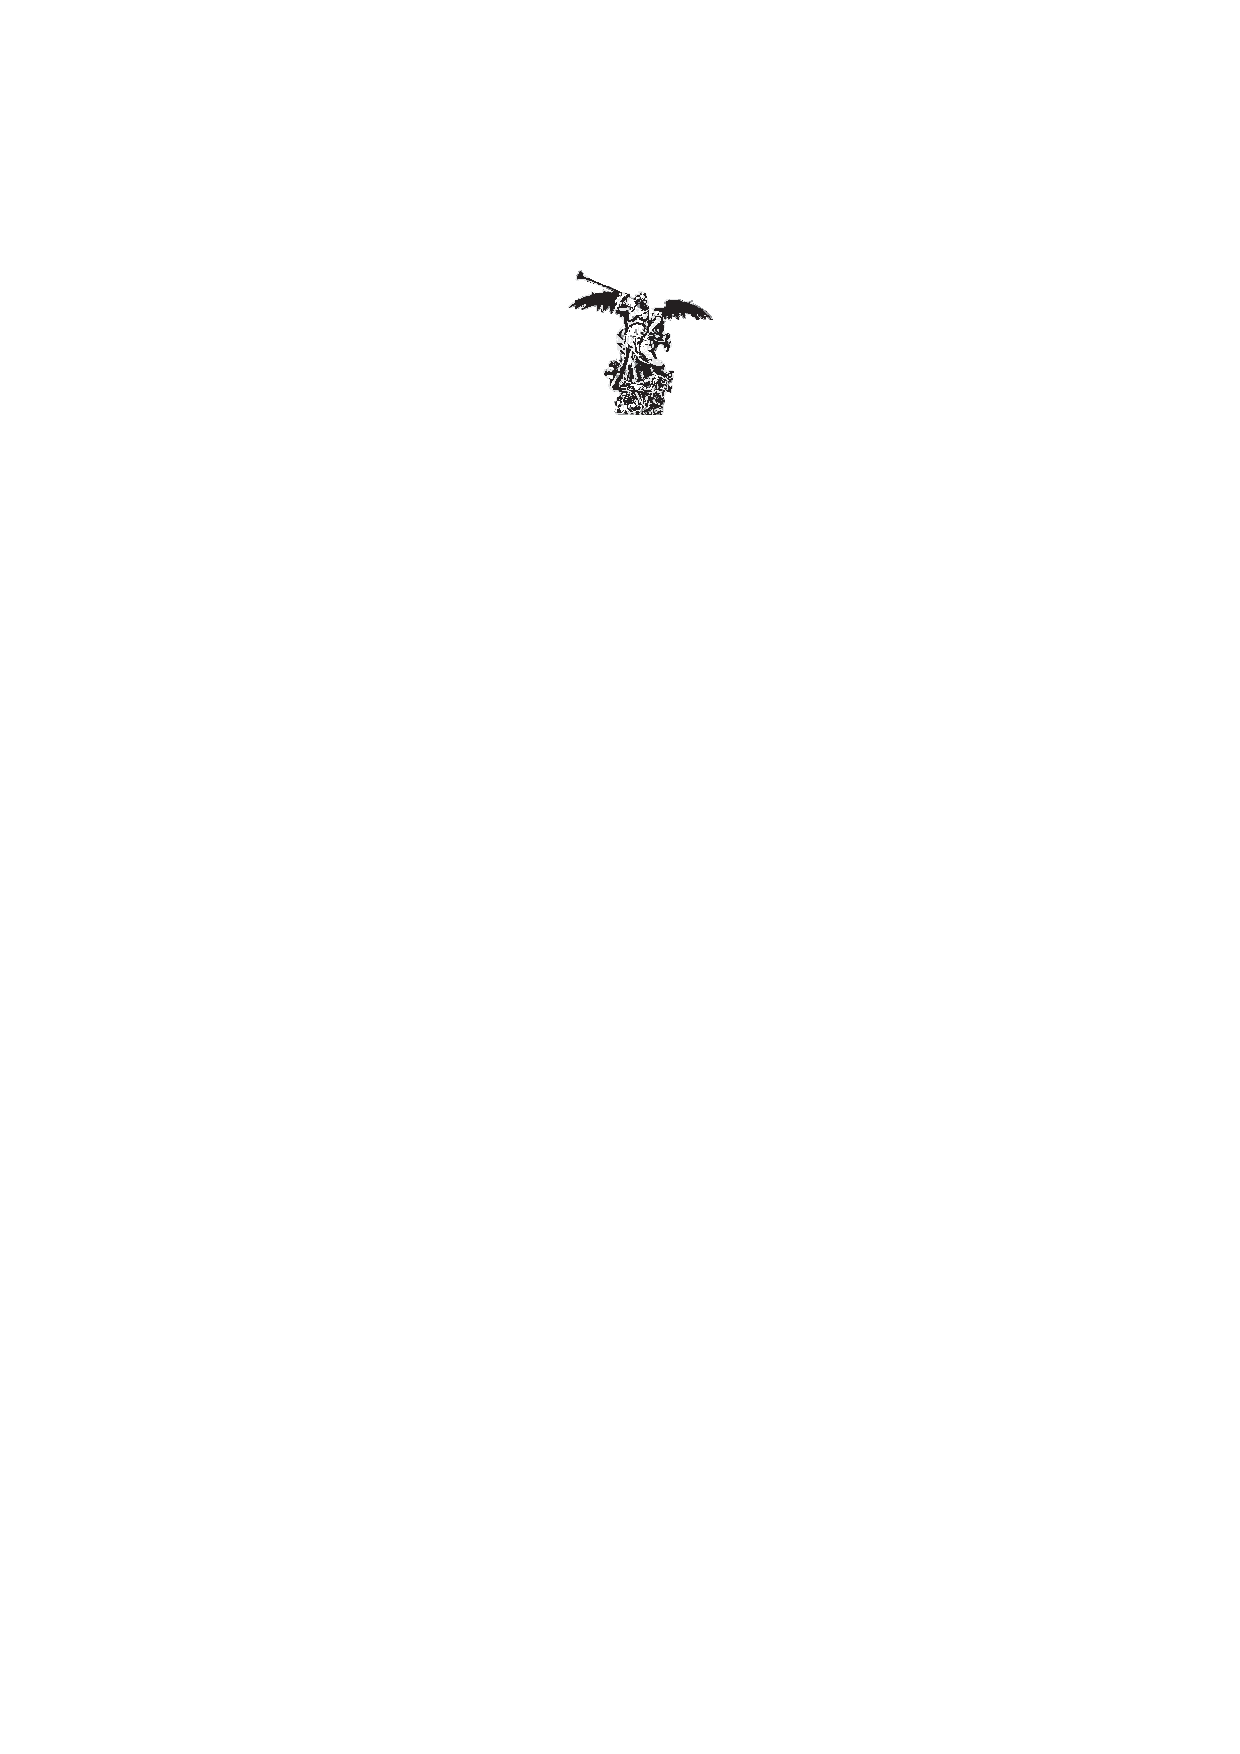
\includegraphics[width=1.9\textwidth]{images/famaNegro}%
\vfill
}}
%  cambiar el factor de transparencia para que salga más o menos claro
\put(0,0){\transparent{0.85}\textcolor{white}{\rule{\paperwidth}{\paperheight}}}
}
\begin{center}

\includegraphics[width=7cm]{./images/logotipo.jpeg}
\rule{\textwidth}{1.2pt}
DEPARTAMENTO DE QUÍMICA FÍSICA
\par
Programa de Doctorado de Química Teórica y Computacional

\vspace{4cm}

\begin{DoubleSpace}{\LARGE Computational Chemistry of Actinoids in Solution and Confined Media}
\end{DoubleSpace}
\end{center}

\vspace{2cm}

\begin{flushright}
{\Large
Sergio Pérez Conesa}\\
{\large Sevilla, 2019}
\end{flushright}

%%%%%%%%%%%%%%%%%%%%%%%%%%%%%%%%%%%%%%%%%%%%%%%%%%%%%%%%%%%%%%%%%%%%%%%%%%%%%%%%%%%%%%%%%%%%%%%%%%%

\newpage
\mbox{}
\thispagestyle{empty} % para que no se enumere esta página

\newpage
\thispagestyle{empty}

\begin{center}

\includegraphics[width=7cm]{./images/logotipo.jpeg}
\rule{\textwidth}{1.2pt}
DEPARTAMENTO DE QUÍMICA FÍSICA
\par
Programa de Doctorado de Química Teórica y Computacional
\vspace*{0.5cm}

Memoria presentada para optar al Grado de Doctor\\
 en Química por la Universidad de Sevilla.
%\par %Descomentar si no se ponen firma
\vspace*{0.3cm} %0.3 si firma digital
%\vspace*{2.3cm} %2.3 de lo contrario
\begin{center}
\includegraphics[width=2.70cm]{./images/firma_SPC.png}
\end{center}
Sergio Pérez Conesa
\rule{\textwidth}{1.2pt}
\vspace*{0.4cm}%0.4 si firma digital. 2.4 de lo contrario
%\vspace*{2.4cm}%2.4 de lo contrario
V$^\circ$ B$^\circ$ Directores de la Tesis
\par
\vspace*{0.5cm}
\includegraphics[width=2.70cm]{./images/firma_ESM.png}
\hspace*{3.5cm}
\includegraphics[width=2.0cm]{./images/firma_JMM.png}
\newline
Dr. Enrique Sánchez Marcos \hfill Dr. José Manuel Martínez Fernández
\rule{\textwidth}{1.2pt}
\end{center}

\newpage
\ 
\newpage
\thispagestyle{empty}
\vspace*{\fill}
\begin{center}
\begin{minipage}[c]{0.7\textwidth}
Me da vértigo el punto muerto\\
y la marcha atrás,\\
vivir en los atascos,\\
los frenos automáticos y el olor a gasoil.\\
Me angustia el cruce de miradas\\
la doble dirección de las palabras\\
y el obsceno guiñar de los semáforos.\\

Me arruinan las prisas y las faltas de estilo,\\
el paso obligatorio, las tardes de domingo\\
y hasta la línea recta.\\
Me enervan los que no tienen dudas\\
y aquellos que se aferran\\
a sus ideales sobre los de cualquiera.\\
Me cansa tanto tráfico\\
y tanto sinsentido,\\
parado frente al mar mientras que el mundo gira.\\


Francisco M. Ortega, (Fragmento en videoclip Standby de Extremoduro)\\
\end{minipage}
\end{center}
\vspace*{\fill}



\chapter*[Agradecimientos]{Agradecimientos}
Todos los químicos conocen el trabajo de Douglas Hartree, uno de los físicos padres de la química y 
la física cuántica molecular. Pocos en cambio conocen a su padre, William Hartree y a él todos los 
químicos deberíamos también estarle muy agradecido. Hartree padre, que era profesor de ingeniería 
jubilado, ayudó a su hijo a calcular numéricamente las soluciones a las equaciones de Hartree hijo, 
un trabajo muy arduo en esos tiempos. A parte de a su padre, Douglas Hartree debería estar muy 
agradecido a su madre, que era activista de los derechos de la mujer, por la educación en valores 
que seguramente le dio. Y probablemente le deba también mucho a su mujer que le alegraba cuando el 
trabajo le desanimaba o porque simplemente le hacía feliz. 

Yo también quiero darle las gracias a todas las personas que en mayor o menor medida han 
contribuido a que presente esta tesis ayudándome directa o indirectamente:
\begin{itemize}
 \item Al profesor Enrique Sánchez Marcos por hacer posible esta tesis y por todas las cosas que me 
ha enseñado sobre química física y la investigación. 
 \item Al profesor José Manuel Martínez la persona de la que más he aprendido dinámica molecular y 
mecánica estadística y que ha hecho que sea mi parte favorita de la química teórica.
 \item Al profesor Rafael Rodríguez Pappalardo, el ``señor Lobo'' del grupo porque soluciona 
todos los problemas.
 \item Al Dr. Francisco Torrico que comenzó la aventura actínida del grupo y sin la cual esta 
tesis no habría sido posible.
 \item A mis antiguos compañeros de grupo Noelia y Dani por ayudarme al llegar al grupo y por 
enseñarme XAS. 
 \item Al professor Michele Parrinello por acogerme en su laboratorio y enseñarme 
tantas cosas sobre metadinámica y más.
 \item Al Dr. Pablo Piaggi por hacer conmigo parte del trabajo de esta tesis y hacerme la estancia 
en Lugano mas alegre.
 \item Al resto del grupo del prof. Parrinello por hacer que mi estancia en Lugano fuera estupenda 
y por ayudarme desinteresadamente en mi proyecto. 
 \item A Juanín por hablar tanto rato sobre las cosas de esta tesis tomando cervezas.
 \item A mi hermana por hacerme la portada y otros de los gráficos de la tesis.
 \item A mis padres y mi hermana de nuevo porque siempre habéis apoyado mi educación y porque 
quien soy es en gran medida gracias a vosotros.
 \item A la memoria de mis abuelos y a mis abuelas. Se que les hará mas ilusión aún que a mí.
 \item A mi novia Mari Ángeles porque eres la que me ha sufrido y apoyado durante estos cuatro 
años. Porque nunca olvidaremos lo bien que nos lo pasamos en Suiza. Porque estos años sin ti no 
habrían sido tan maravillosos. Porque en todo momento me haces muy feliz.
\end{itemize}

          % Capítulo 1

\selectlanguage{english}

\pagestyle{index}
\cleartorecto
\tableofcontents % Indice general. Incluye automáticamente chapter, section, subsection...
\cleartorecto
\listoftables    % Indice de tablas. Incluye automáticamente tablas.
\cleartorecto
\listoffigures   % Indice de figuras. Incluye automáticamente figuras.
\newpage
%\glsaddall[types={acronym}] Si quieres que los acrónimos se definan antes del texto
%%%%%%%%%%%% UNCOMMENT
%\printacronyms % input files created by makeindex

%%%%%%%%%%%%%%%%%%%%
\setcounter{secnumdepth}{0}      % Profundidad hasta la que se numeran secciones,subsecciones,
                                 % si se pone a 0 no numera.
\chapter*{Abstract}
\markboth{Abstract}{Abstract}
\addcontentsline{toc}{chapter}{Abstract}
The nuclear power industry accounts for around 10\% of the electricity production worldwide and 
up to 70\% in some countries.\cite{NuclearElectricEnergy} One of the problems of this otherwise 
clean energy source is 
the generation of high level radioactive waste which remains harmful for 
centuries.\cite{NuclearesLozano} 
Spent nuclear fuel is reprocessed to extract the actinoids that are still fissile (U  and 
Pu) 
from highly radiotoxic minor actinoids (Np and 
Am).\cite{NuclearesLozano,HERBST2011141,Katz2007-ch24} This is done typically through the  
PUREX process which is based on liquid-phase extraction of actinoids based on their 
physico-chemical properties. Some of the most important species in this process are the actinyl 
hydrated cations, \ce{[AnO_2*(H2O)5]^{2+/+}(aq)]} for An=U,Np,Pu,Am. The actinyls are linear 
oxo-cations formed by the oxidation states V and VI of the metal. High level radioactive waste 
resulting from the PUREX process are destined to be kept underground in permanent geological 
repositories for the centuries to come.\cite{NuclearesLozano} These repositories use clays as liner 
materials to prevent 
potential diffusion of radioelements to the environment.\cite{Delage2010} The main clay component 
 is montmorillonite clay.\cite{Delage2010} In this thesis we will study the physico-chemical 
properties of actinyl cations in aqueous solution and in clays using computational chemistry . 

In order to run molecular dynamics simulations (MD), \textit{ab initio} force fields were developed 
for 
U(VI), Np(VI), Np(V), Pu(VI) and Am(VI) in water. One additional force field was developed for the 
interaction 
of uranyl with the montmorillonite clay aluminosilicate layers. The force fields 
are based on the hydrated ion model\cite{JPhysChem_ESM_1993,JChemPhys_ESM_1998,JACS_ESM_1999} 
developed by the group in the mid 90's. This model accounts 
for many-body effects like polarization and charge transfer in a non-polarizable framework. Its 
main characteristic is to consider the hydrated ion and not the naked ion as the solute. In this 
way, 
first-shell water molecules and bulk water molecules are different species. This allows 
the assignment of different atom types, partial charges and interaction potentials to the 
first-shell than to 
bulk water molecules. It additionally parametrizes explicitly hydrated ion bulk-water 
molecule interactions. 

Once the force fields were developed, MD simulations of the actinyls in water were 
run. The simulations reproduced satisfactorily a wide variety of physico-chemical properties of the 
system: hydration enthalpy, vibrational spectra, diffusion coefficients, XAS spectra, etc. This 
was 
a sign of the robustness of our force field development strategy.  The first conclusion drawn from 
the simulations is that the solvation structure of the 
different actinoids is almost indistinguishable one from the other. Furthermore, despite the 
charge difference between \ce{[NpO2]^{2+}} and \ce{[NpO2]^{+}}, their solvation resembled strongly. 
We observed that the equatorial solvation of the actinyls was equal to most 
conventional cations: 
the first-shell forms two hydrogen bonds with bulk water molecules. In contrast, the \oyl atom 
solvates hydrophobically: water \newline molecules surround it forming hydrogen bonds with 
other 
solvent molecules but not with \oyl. We concluded that the actinyl cations are highly anisotropic 
amphiphillic cations that have a conventional hydration sphere caped at the poles by hydrophobic 
solvation regions. 

The theoretical EXAFS spectra of the actinyls were  calculated and compared to experiment. 
For uranyl, the theoretical-experimental agreement is good. For the rest of actinyls the 
reproduction is less satisfactory, particularly in the case of the triplet 
cation, \ce{[NpO2]^{2+}}. The force fields 
for these
cations were developed at the DFT level of theory. With the aim of improving performance, the 
explicit treatment of static correlation was then taken into account. A 
NEVPT2\cite{NEVPT2_1,NEVPT2_2,NEVPT2_3} force field was developed for the 
\ce{[NpO2]^{2+}}-\ce{H2O} interaction. The effect of this increase in level of theory was 
studied, and the decomposition of 
the complex EXAFS signal was shown to be useful in the understanding of the main EXAFS spectrum 
features. 

\begin{figure}[ht!]
     \centering
         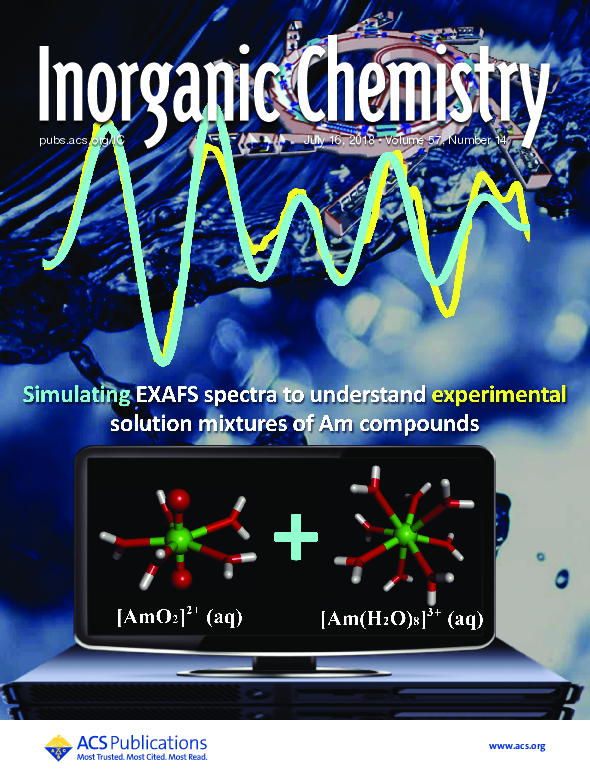
\includegraphics[width=0.5\textwidth]{images/cover_IC2018.png} 
        \caption[Cover Inorganic Chemistry]{Cover of Inorganic Chemistry for the work ``Extracting 
the Americyl Hydration from an Americium Cationic Mixture in Solution: A 
Combined X-ray Absorption Spectroscopy and Molecular Dynamics Study'' presented in this thesis
.\cite{Perez-Conesa2018} }
        \label{cover1}
\end{figure}

Due to its chemical instability, americyl (\ce{[AmO2]^{2+}}), has never been isolated in aqueous 
solution. As a result, the only EXAFS spectrum of \ce{[AmO2]^{2+}} corresponds to a 70/30 mixture 
of 
americyl and \ce{Am^{3+}}.\cite{JRadioanNucChem_Riddle_2016}  We simulated the 
EXAFS spectra of both species from their respective MD simulations and weighted them into a single 
spectrum to produce a simulated EXAFS 
of a mixture of species\cite{Perez-Conesa2018}. The good comparison of the simulated spectrum 
and experiment allowed us to 
predict theoretically the structural parameters and EXAFS spectrum of a pure americyl solution, a 
solution yet to be obtained experimentally\cite{JPC_SPC_2017}. The same procedure was applied 
to the XANES spectrum. This 
work was featured in the cover of the issue 57 of  Inorganic Chemistry of 2018, Figure
\ref{cover1}.



The MD simulations of the uranyl hydrated ion in the aqueous interlayers of 
montmorillonite clays gave interesting microscopical details of the system hard to 
obtain experimentally\cite{JPC_SPC_2017}. The simulations reproduced the few experimental 
microscopical information of 
the system: the uranyl hydrated ion interacts with the surface through the formation of an 
outer-shell complex\cite{GeoCosmoAct_Catalano_2005} and the uranyl axis is neither perpendicular nor 
parallel to the surface\cite{MinWatIntClEq_Denecke_1999}. We 
calculated for the first time from a MD simulation the constrictivity factor, 
$\delta_{int}$, which was found to be near the right order of magnitude to experiment. Strong 
interaction sites for uranyl were found on the clay. These sites are groups of three magnesium 
substitutions around which uranyl cations are electrostatically attracted. As a 
consequence the diffusion of uranyl in the clay exhibits a hopping diffusion mechanism. 
Because of this, the diffusion of uranyl increases with increasing 
uranyl concentration due to cation-cation interactions and a larger coverage of 
surface sites. This work was featured in the cover of the issue 121 of the Journal 
of Physical 
Chemistry C of 2017, Figure \ref{cover2}. In addition it was chosen best article of a young member 
of the ``Specialized Group of atomic and molecular physics'' (GEFAM) of the Royal Spanish 
Society of Physics in 2017.

\begin{figure}[ht!]
     \centering
         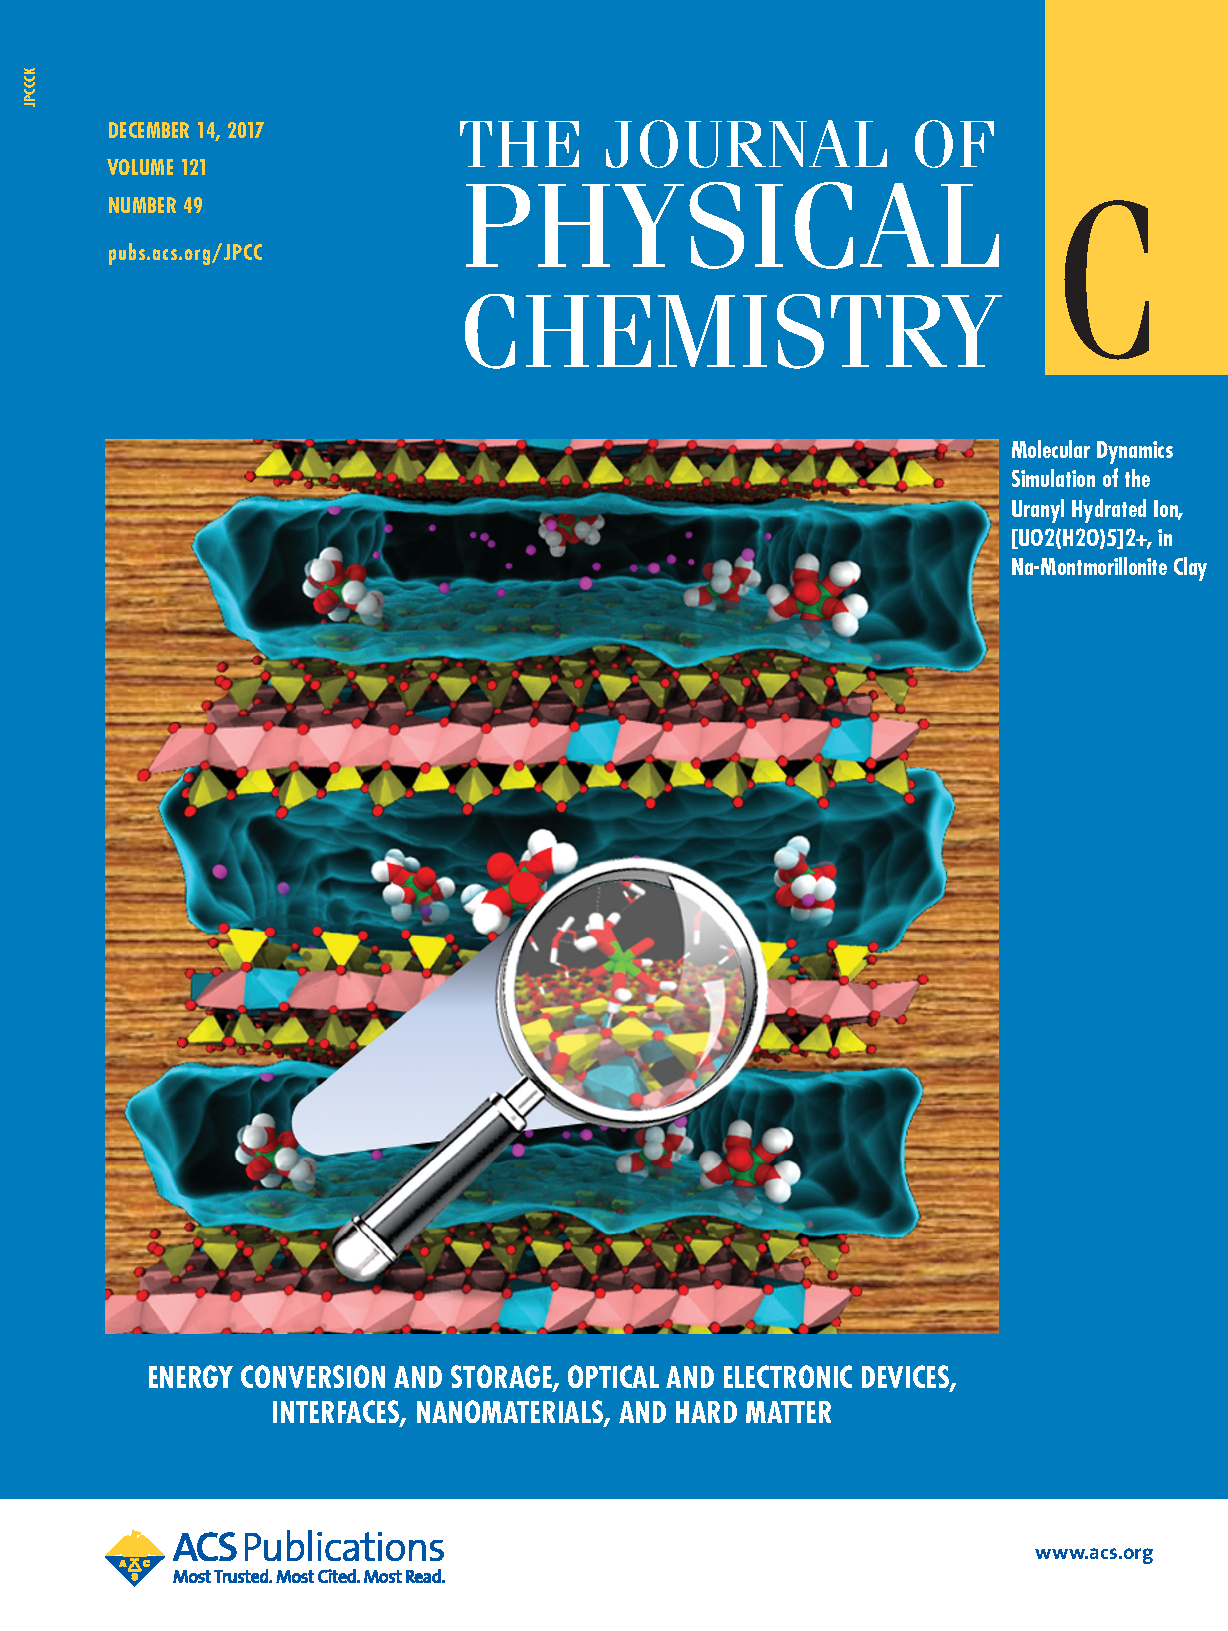
\includegraphics[width=0.5\textwidth]{images/cover_JPCC2017.pdf} 
        \caption[Cover Journal Physical Chemistry C]{Cover of the Journal of Physical Chemistry C 
for the work ``Hydration and Diffusion Mechanism of Uranyl in Montmorillonite Clay: Molecular 
Dynamics Using an Ab Initio Potential'' presented in this thesis.
\cite{JPC_SPC_2017} }
        \label{cover2}
\end{figure}

Finally, a simple local fingerprint for 
hydrophobicity/hydrophilicity was developed. This fingerprint is inspired by the expansion of 
the 
entropy of a system as a sum of terms of increasing correlational 
order.\cite{nettleton1958expression,baranyai1989direct} The fingerprint, which refers to the 
translational component of the entropy, 
measures the hydrophobicity/hydrophilicity of individual atoms of a solute taking as input its 
radial distribution function with water. The fingerprint classifies satisfactorily, the atoms of 
the amino acids. Nevertheless, the fingerprint has mixed results in classifying the atoms of 
the actinyl pentahydrates. A future improved fingerprint should probably make use of orientational 
pair entropy in addition to some techniques to consider the anysotropicity of the solute in 
complex 
environments. Additionally, the fingerprint proved to be a useful solvation/desolvation 
collective variable for enhanced sampling simulations. 

\bibliographystyle{achemso}
\bibliography{./library,./extrabib}     % Abstract

\mainmatter
\setcounter{secnumdepth}{3}      % Pone numero hasta las subsecciones
\maxtocdepth{subsubsection}      % Incluye en el indice las subsubsecciones

\pagestyle{mypagestyle}
\ChapFrame
\selectlanguage{english}
%%%%%%%%%%% Capitulo 2 Metodologia %%%%%%%%%%%%%%%%%%%%%%%%%%%%%%%%%%%%%%%%%%%%%%%%%%%%%%%
\setcounter{chapter}{0}
\chapter[Introduction]{Introduction}\label{c1:intro}
As you read over these lines a significant amount of the energy used by the light-bulb 
illuminating these pages is produced by the splitting of 
uranium and plutonium nuclei. 20\% if you are right now in Spain, the USA or 
the United Kingdom, 30-40\% if you are in the Czech Republic, Finland, Belgium, South Korea, 
Sweden or Switzerland and a world record of 77\% produced by state-owned company if you are 
in France.\cite{NuclearElectricEnergy} Even if you are reading this from Italy where nuclear 
energy has been forbidden, part of the energy you are consuming is nuclear since it is bought from 
the French nuclear 
industry.

Regardless of 
the reader's opinion on the nuclear power industry, it undoubtedly is an industrial leviathan 
that should be understood if only for the sake of nuclear security.  In this chapter we will 
make an effort to overview some aspects of the industry and how understanding the 
chemical nature of some of its essential substances is still relevant 70 years after the first 
nuclear reactor developed by Enrico Fermi himself. 

\section{Nuclear Power}

In 1939, Otto Hanh, Lise Meitner  and Otto Robert Frisch discovered and described the fission 
of uranium on the basis of the ``liquid drop'' model of the nucleus. Hanh
received the Nobel Prize in Chemistry for the experimental discovery. Unfortunately Meitner 
and Frisch who explained the physics behind did not. The essential idea of fission is that the 
nucleus of \ufis is metastable and the impact of a slow neutron can split it into more stable 
smaller 
nuclei. The sum of daughter nuclei masses is lower than that of \ufis \newline and 
the difference in mass is converted into tremendous amounts of energy according to Einstein's 
famous equation: $E=mc^2$. Two or three neutrons are also emitted in the process which 
depending on their speed might impact another \ufis nucleus and continue the chain reaction 
over and over.

If the concentration of \ufis is extremely high the reaction advances exponentially leading
to a sudden splitting of all the fissile nuclei and a nuclear explosion occurs. To obtain 
this critical concentration of the nuclear material generally, another conventional explosion 
must be used to compress the nuclear explosive. This is the basis of a fission nuclear bomb: 
an explosion within the bomb compresses the fissile material (uranium or plutonium) into 
critical density which releases in a split second most of its nuclear energy. This was the 
mechanism used in the bombings of Hiroshima and Nagasaki during World War II. 

The energy of fission can also be used to generate electricity by controlling the 
nuclear reaction. Uranium or plutonium act as fuel and not as explosives. The nuclear fuel is 
composed in most cases of \ce{UO2}(s) with varying ratios of \ufis/\unofis. At ordinary 
densities it generates no energy. Spontaneous fission of \ufis generates 
neutrons that are fast and inefficient in splitting other nuclei. But if we introduce a 
moderator material (typically graphite, water or heavy water) the neutrons can scatter on the 
nuclei of the moderator slowing them down and making the thermal (slow) neutrons effective in 
splitting fissile 
nuclei. This promotes fission and a chain nuclear reaction is formed generating energy. The 
growth of the energy emitted is exponential and must be reduced. For this, another material 
captures the excess neutrons and reduces the rate of fission controlling the reaction and 
avoiding a nuclear accident. These materials are substances that are effective in capturing 
neutrons, for example cadmium or boron, and are know as control materials. In this way, the fuel is 
steered 
into steady reaction. The energy liberated heats water surrounding the reactor 
vessel which in the form of steam moves turbines and a generator converts the kinetic energy 
into electricity. 

Nuclear energy is a cheap and \ce{CO2}-free source of energy using a fuel that is 
fairly abundant, 40 times more than silver. In addition, unlike fossil fuels, the uranium 
ores are fairly evenly distributed by countries according to the Organization for Economic 
Co-operation and Development (\gls{oecd})\cite{UReserves}. Then, why is not nuclear energy the main 
source of electricity in the world? The reasons are all derived by the terrible effects that 
radiation and radioactivity can cause on human beings and the environment. Three main reasons 
can be argued: 

\begin{itemize}
 \item The sometimes reasonable and sometimes unreasonable fear of the po\-pu\-lation of 
anything 
containing the adjective 
``nuclear''. This is the reason why doctors ask their patients to have a Magnetic Resonance 
Imaging (MRI) which should actually be called Nuclear Magnetic Resonance 
Imaging. Ironically, unlike in other medical techniques no radioactivity is involved in MRIs. 
 \item The occurrence of three major nuclear power accidents: Three 
Mile Island (1979), Chernobyl (1986) and Fukushima (2011).
 \item The generation of highly radioactive nuclear waste that must be processed safely and 
adequately to be kept afterwards for centuries undisturbed in geological facilities. 
\end{itemize}

About the first two reasons this work will not dive into but we refer to the excellent books of 
Prof. Lozano 
Leyva\cite{NuclearesLozano,FukushimaLozano}. 

\section{Nuclear Fuel, Nuclear Waste and Nuclear Cemeteries}
\begin{figure}
     \centering
         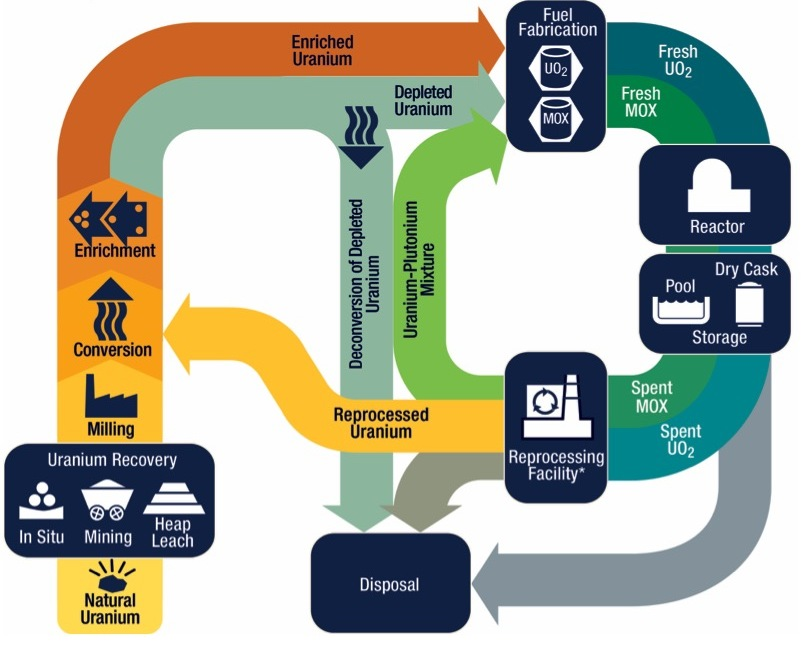
\includegraphics[width=0.8\textwidth]{images/The_Nuclear_Fuel_Cycle.jpg} 
        \caption[Nuclear Fuel Cycle]{Schematic representation of the nuclear fuel cycle from the 
mine to disposal.\cite{NuclearFuelCycle} }
        \label{FuelCycle}
\end{figure}

Nuclear fuel is mostly \ce{UO2(s)}. The useful fissile isotope 
is \ufis but it is only the 0.7\% of natural uranium being 99\% of it \unofis. For this 
reason, many reactors run 
uranium enriched in \ufis up to 1-3\%. Additionally, plutonium can also become fuel for several 
designs of reactors. This plutonium can be obtained from the dismantlement of thermonuclear 
bombs, also known as H-bombs, that use a 
plutonium fission explosion to initiate a fusion chain reaction of deuterium and tritium. 
Additionally,  during power generation in a nuclear power plant, the neutron 
capture of uranium generates plutonium. This plutonium can be recovered from 
spent uranium fuel, an extraction known as 
reprocessing. Plutonium and depleted uranium can be used in some nuclear reactors in the form 
of mixed oxides in a material known as \gls{mox}. Finally, there is a high interest in the 
substitution of uranium and plutonium fuels by thorium\cite{thorium} which would have 
significant advantages: it is more abundant and efficient than uranium, produces less harmful 
byproducts and cannot be used  to make weapons. But the most important feature of the thorium 
chain reaction is that there is no possibility of a meltdown like in Chernobyl making it much 
safer than the uranium alternative. Unfortunately thorium technology is still under development 
and while uranium remains cheap the incentives to fully develop thorium technologies are low. 
Figure \ref{FuelCycle} represents the cycle of uranium from the mine to its disposal.

High level radioactive waste is made by nuclear power plant residues
which are the result of the fission of the fuel. They contain unstable nuclei that  
emit alpha, beta or gamma radiation. Nuclear fuel is much more radioactive and dangerous when 
it has already been spent. For this reason 
reprocessing is a much more environmentally dangerous step than the actual power production. 
In spite of this, 
there has never been any accident in the handling and permanent storage of high level 
radioactive waste.

\begin{table}[h!]
\caption[Composition of spent nuclear fuel]{Typical composition of spent nuclear fuel from a 
uranium nuclear 
power plant.\cite{NuclearesLozano}}\label{comp}
\centering
{\small
\begin{tabular}{ll}
\toprule
95.6\% &$^{232}$U: 0.1-0.3\%; $^{234}$U: 0.1-0.3\%; $^{235}$U: 0.5-1.0\%; $^{236}$U: 
0.4-0.7\%; \unofis : rest \\
2.9\% &Stable elements.\\
0.9\% &Pu.\\
0.3\% &Cs and Sr (fission fragments).\\
0.1\% &I and Tc (fission fragments).\\
0.1\% &Long-lived fission fragments.\\
0.1\% &Np, Am and Cm (long-lived transuranium elements).\\
\bottomrule
\end{tabular}}
\end{table}


Reprocessing extracts uranium and plutonium from the waste to feed the reactor and separate 
radiotoxic elements for its permanent disposal. Spent nuclear fuel composition is summarized 
in Table \ref{comp}. The main problem of reprocessing is the complexity of the mixture 
including a wide variety of elements and isotopes some of them chemically very similar like the 
actinoids. 
If reprocessing is done, which is not always the case for economical reasons, it is done 
normally using the \gls{purex} method (Plutonium Uranium Redox 
EXtraction).\cite{NuclearesLozano,HERBST2011141,Katz2007-ch24} 

The PUREX method was developed as a part of the Manhattan project at the Oak Ridge National 
Laboratories and its initial goal was to purify plutonium for its use as a nuclear weapon 
detonant. The first step of PUREX is to dissolve the solid nuclear fuel pellets in 
concentrated nitric acid. Then Pu and U are extracted using liquid/liquid extraction. The 
original aqueous phase is exposed to a hydrocarbon phase in the presence of a complexating 
agent, mainly, tri n-butyl phosphine (\gls{tbp}):
\begin{align*}
&\ce{[UO_2*(H2O)5]^{2+}(aq) + 2NO3^-(aq) + 2TBP(org) <=> [UO_2(NO3)2*(TBP)2](org) }\\
&\ce{[Pu*(H2O)_n]^{4+}(aq) + 4NO3^-(aq) + 2TBP(org) <=> [Pu(NO3)4*(TBP)2](org) }
\end{align*}
TBP is highly selective for oxidation states VI and IV and virtually has no affinity for 
states III and V (Np(V), Am(III), Cm(III), etc.). The extraction is nearly 
quantitative and highly selective. The organic phase is then treated with reducing agents to 
reduce Pu(IV) to Pu(III) which is extracted with another aqueous phase with a very high yield. 
The resulting Pu and U solutions are then purified, evaporated and the actinoids are converted 
into oxides to be reused as nuclear fuel. The key chemical point in the 
process is the stability of \ce{[UO_2]^{2+}} and the chemical and electrochemical flexibility 
of the Pu ions. The original aqueous phase contains all the highly radioactive elements, most 
importantly highly radiotoxic actinoids like Cm, Am and Np.  Although the basic chemical ideas 
behind PUREX are simple, in practice it is a very complex chemical engineering process.

The final waste generated from PUREX contains the very radioactive but non-fissile 
nuclei including several transuranium actinoids (Np, Am and Cm mostly). This radioactive waste is 
the smallest by far in volume of all radioactive waste of industry but concentrates most of 
the sample radioactivity: 99.9\%. For this reason they are known as High Level Radioactive 
Waste 
(\gls{hlrw}).\cite{OECD-NEA-HLRW}

\section{High Level Radioactive Waste Permanent Storage}

HLRW is kept in waste pools close to the reprocessing or nuclear power plants allowing them to 
cool off with water acting as a radiation barrier. These materials 
can be then vitrified or solidified and introduced in stainless steel containers and allowed 
cooling for up to 50 years before their permanent disposal. The radioactive activity of the 
containers will remain terribly harmful for hundreds of thousands of years. 

Several solutions have been proposed to conceal for the centuries to come the HLRW: underground 
geological permanent storage, deep sea ground storage, glacier storage in Antartida, sending it 
to 
outer space or transmutation into harmless nuclei. Even though transmutation would be the ideal 
solution, unless major breakthroughs occur, Science is decades away from that kind of 
technology. 
The best agreed solution is storage in geological underground permanent 
disposal sites. Geological permanent storage sites are chambers dug deep underground in the rock 
where the containers will be stored safely for the centuries to come. The construction would 
be done in geologically stable locations and the rock would conceal the radioactive matter 
and its radiation. The rock acts as a passive barrier and also prevents any water from
leaking in or out of the repository. 

Most countries do have nuclear permanent disposal sites to keep mid and low level radioactive waste 
generated by the non-nuclear industry, research, radiomedicine etc. Nevertheless, even though the 
amount of HLRW has been growing since the beginnings of nuclear power production  a fully functional 
HLRW permanent geological disposal site is still missing. Many countries have 
plans to build it. Finland will be the first country to have a geological HLRW disposal 
site, Onkalo, 
in Posiva which is expected to become operative in 2023.\cite{OECD-NEA-HLRW}

The security of the facilities must be extreme. Specially because the nuclear containers remain hot 
for hundreds of years and are exposed to severe radiation damage. The sites should be air-tight 
particularly to prevent the entrance of water that could disperse the radioelements into the 
underground streams. 

\begin{figure}
     \centering
     \subfloat[a)]{{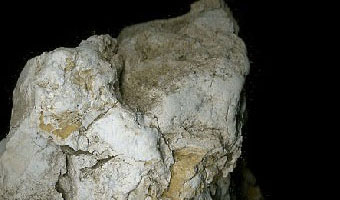
\includegraphics[width=7.5cm]{images/MMT_rock.jpg} }}%
     \\
     \subfloat[b)]{{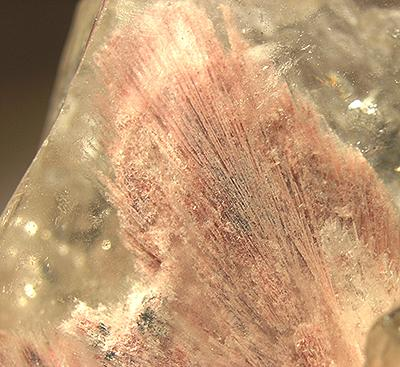
\includegraphics[width=7.5cm]{images/MMT_cris.jpg} }}%
     \caption[Montmorillonite clay minerals]{a) Montmorillonite clay rock. b) Montmorillonite 
clay crystals embedded in quartz.\cite{MMT_mac1,MMT_mac2}}
     \label{clay}
\end{figure}


\begin{figure}
     \centering
         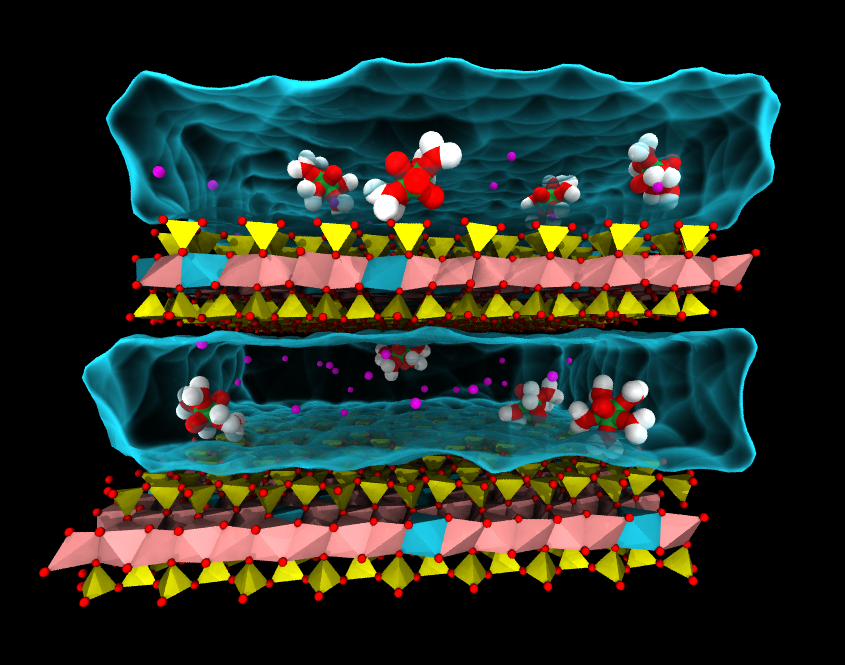
\includegraphics[width=0.8\textwidth]{images/clay} 
        \caption[Hydrated montmorillonite clay containing uranyl cations]{Unit cell of hydrated 
sodium montmorillonite clay containing uranyl hydrated ions, \ce{[UO2*(H2O)5]^{2+}}, in the 
interlayer. The water bulk water molecules are omitted and represented as a blue transparent 
surface. The uranyl cations are drawn with the ``licorice'' representation. \ce{SiO4} tetrahedra 
(yellow), \ce{AlO6} octahedra (pink) and \ce{MgO6} (blue) are represented as polyhedra. The atoms 
are colored as follow: O (red), H (white), \ce{Na^+} (purple) and U (green). }
        \label{clay2}
\end{figure}

Clays are particularly suited both as natural host rock or natural barrier for the permanent 
geological HLRW site and as liner material or artificial barrier to conceal the 
repository.\cite{Delage2010} The most used clay rock is bentonite which is primarily 
composed of montmorillonite clay (Figures \ref{clay} and \ref{clay2}). Bentonite is compacted 
and mixed with sand 
and serves as an 
artificial barrier surrounding the horizontal galleries which hold the HLRW. Clays are selected 
for three reasons: their high thermal conductance to dissipate the heat generated by the 
waste radioactivity, its low permeability to water and its high retention of radionucleides. 
This high retention of radioelements is due to their ionic exchange capability. If the
clay is exposed to a cation containing solution it would release its harmless \ce{Na+} cations and 
absorb radioactive cations such as actinyls.

\section{Hydrophobic Solvation}\label{sec:hydrophobicity}
In this section, we will make a small detour from the actinoids to talk about hydrophobic solvation 
which shall be relevant in the study of actinyl solvation and the development of the hydrophobicity 
and hydrophilicity fingerprint.

``Like dissolves like'' is one of the first concepts a chemist learns in relation to the 
solvation 
of compounds.\cite{reichardt2011solvents-ch1} It implies that solutes that are chemically like 
water 
will mimic water and be 
hydrophilic. Solutes that are not like water will ``dislike'' water and be 
hydrophobic. The classification of atoms and by extension molecules as hydrophilic and hydrophobic 
has traditionally been done based on chemical experience and heuristics which assign the character 
based on the chemical identity of the atoms. Hydrophobicity and hydrophilicity plays an important 
role in 
processes such as solvation, protein folding, micelle or membrane formation, phase transfer or 
crystallization.  

Hydrophobic solvation has several peculiarities. Hydrophobic compounds have a positive free energy 
of hydration, a negative entropy of hydration, a negative enthalpy of hydration and a large 
positive specific heat of hydration\cite{Harris2016,Ben-Amotz2016}. The word ``hydrophobic'' can 
generate the impression that the interaction of a hydrophobe with water should be repulsive and 
therefore its solvation enthalpy positive. Nevertheless, hydrophobic solutes interact through van 
der Waals interactions with water which are weak compared to water-water interactions but 
attractive. van der 
Waals interactions are non-di\-rec\-tio\-nal so water molecules are free to form a hydrogen 
bond 
network around the solute. Figure \ref{CH4} shows methane in liquid water and how the water 
molecules form their hydrogen bond network around the solute.

Hydrophobic solutes have the tendency to self-aggregate reducing their surface exposed to  
water. This self-assembly is known as the hydrophobic effect. Within chemistry and biochemistry it 
is common to talk about hydrophobic interactions or forces to describe the 
hydrophobic effect but this is misleading and should be avoided\cite{Cremer2017}. It seems to 
suggest 
that there is an intermolecular interaction ``special'' to these systems which have only regular 
van der Waals or hydrogen bond interactions. The hydrophobic effect is a water-mediated 
``self-sorting'' phenomenon. The free energy of water molecules is lower at bulk solution than on a 
hydrophobic molecule surface. The segregation of hydrophobic solutes reduces the amount of water at 
their surfaces producing an overall decrease of free energy of the system. 

The self-assembly \textit{is}
driven by a force, but it must be considered a force only in the ``potential of the 
mean force'' sense. In order words, if there 
is a free energy surface which is a function of a self-assembly collective variable its derivative 
can be 
considered the hydrophobic effect force.\cite{Ben-Amotz2016} Nevertheless, this terminology leads 
to misunderstandings and should ideally disappear. 

\begin{figure}
\centering 
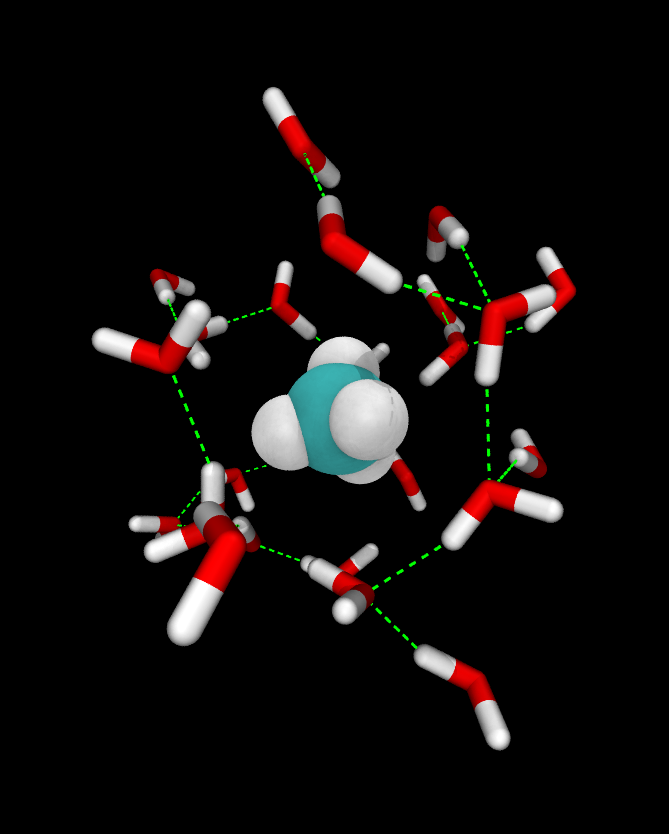
\includegraphics[width=7cm]{./images/CH4.png}
\caption[Hydration of \ce{CH4}]{Snapshot of a MD
simulation of methane in water. 
Only 
nearest water molecules are shown. The water molecule forms its hydrogen bond network around the 
cavity generated by methane in the solvent. }
\label{CH4}
\end{figure}

It has long been known that for small hydrophobic solutes at room temperature the entropic term 
dominates the free energy of 
solvation and is the reason for the low solubility of hydrophobic molecules in 
water.\cite{Chandler2005} This was explained theoretically in the works of Hummer et 
al\cite{garde1996origin,hummer1996information} on hydrophobic solvation. Their works started a body 
of theory known as ``Information Theory'' of hydrophobic solvation. Information Theory models the 
hydrophobic solute as a cavity in water. This cavity can be explicitly generated in solution by 
introducing a hard sphere particle or by the isomorphic problem of studying spontaneously generated 
cavities in water.

The cavity generated by hydrophobic solutes disrupts the hydrogen bond network of water decreasing 
the number of allowed microstates and thus the entropy of the solvent. Interestingly, this happens 
without affecting the average number of hydrogen bonds 
formed by the solvent around small 
solutes.\cite{Pratt1977,KaLum1999,Huang2001,Huang2002,Chandler2005} For this reason 
the hydration entropy of small hydrophobic \newline molecules correlates with molecular volume. 
This picture relates to the classical notion of hydrophobic solvation proposed by Frank and Evans 
in 
1945, the ``Iceberg'' model of hydrophobic solvation. In this model, the 
structure of water around a hydrophobic solute is reinforced and the dynamics slowed down by the 
formation of an ice-like cage of water molecules\cite{frank1945free}.

If the molecular size is high ($\sim$\SI{1}{\nano\meter}) a water/vapor-like interface is 
generated\cite{Willard2014} and the hydration entropy correlates with the 
molecular 
surface area instead of volume.\cite{Chandler2005} The reason is that water on the solute surface 
cannot form in this case the average number of hydrogen bonds it forms in solution.

Unlike hydrophobic solvation of small 
molecules at room temperature, the hydrophobic effect can be enthalpy driven, entropy driven or 
both\cite{Cremer2017,Chandler2005}. Quoting David Chandler: 

``The increase in molecular self-assembly of hydrophobic solutes with temperature is often cited as 
implying that hydrophobic interactions are entropic. Entropy does indeed contribute, but the
assembly process is driven by the difference between the entropically dominated solvation free 
energy of small molecules and the enthalpically dominated solvation free energy of large 
surfaces.'' \cite{Chandler2005}

\section{Systems Studied} 

The studies performed during this thesis are based on a simple scientific belief: 
fundamental understanding sheds light on applications. We study several systems important to 
the nuclear industry using fundamental science, for the sake of understanding, but bearing 
in mind the importance an applied scientist might give to our findings. For this reason we 
focus on systems that are interesting in themselves but also of potential relevance in waste 
reprocessing and storage or general actinoid chemistry. 

We studied four elements: uranium, neptunium, plutonium and americium. These four elements 
lie together in the actinoid or $5f$ row and are crucial in nuclear industry as fuels, 
dangerous waste or potential pollutants if accidents happened. We have studied their 
actinyl form, \ce{[AnO2]^{2+/+}} which correspond to oxidation states VI and V, and their main 
species in highly oxidizing and acidic aqueous media. Their study in solution is 
crucial because it is the form in which they are reprocessed and their dangerous mobile form 
if accidents were to occur. We also studied uranyl in clays to study its diffusion in 
the material and how the clay would slow down its diffusion compared to aqueous solution. 

A local example can be put forward with respect to accidents, not of the nuclear power
industry, but rather of the violent use of radioactivity. In 1966, two American military 
aircrafts crashed and 4 termonuclear plutonium bombs were dropped in Palomares (Almer\'ia) 
which is a 4 hour drive away from where I am writing this Thesis.\cite{palomares} Fortunately, only 
the conventional explosive of two of the bombs exploded and no nuclear explosion happened. 
Nevertheless, the explosion dispersed an aerosol of Pu in the nearby area. Although the bombs 
were recovered and part of the contamination cleaned, to this day regions around where the 
bombs landed are under strict nuclear control. One of the problems of Pu is its decay over time 
into Am which is much more volatile and radiotoxic than the rest of actinoids. For this kind of 
reasons, it is very important to understand the apparently obscure chemistry of americium in 
natural media such as clays or water.\cite{Katz2007-ch8}

Besides the nuclear industry, actinoids have a very interesting fundamental 
chemistry\cite{Pichon2017} in terms of bonding, electronic structure and reactivity. 
Understanding the chemistry of 
the compounds can help technological development. Neptunium as of today lacks any practical 
use, but who would have thought that \ce{^{241}Am} would be present in every household smoke 
detector due to its $\alpha$-emition (although they were banned in Spain in 2005). Also, 
though it might sound shocking, uranium is 
a 
naturally occurring element which is 40 times more abundant than silver. Therefore, knowledge 
of its speciation and chemistry in natural waters or clays is important even when its source 
is geological.

Experimental information on actinoids in solution is scarce and hard to 
obtain.\cite{Ions_in_sol_and_Marcus_2016,actinides_solution_v2,chemrev_Altmaier_2013} The 
reason for 
this is their radioactivity which requires 
the use of specialized techniques and specialized facilities.\cite{Pichon2017} 
Theoretical chemistry of actinoids gives many opportunities to study them in an 
inexpensive and safe way. This is the point of view adopted in this thesis: the studies here 
reported have been devoted to the 
computational chemistry of several actinoid cations and their actinyl forms but also in close 
relation to experiment, for example, in the simulation of EXAFS spectra. 

The first article of the compilation deals with the development of an \textit{ab initio} force 
field based on the hydrated ion model\cite{JPhysChem_ESM_1993,JChemPhys_ESM_1998} (\gls{him}) for the 
uranyl pentahydrate, \ce{[UO2*(H2O)5]^{2+}}, in 
solution. The force field allowed us to run classical molecular dynamics (\gls{md}) simulations 
and 
obtain 
interesting \newline in-solution properties of the complex. In particular: to describe the two 
solvation 
behaviors it 
exhibits as well as many spectroscopic, dynamic and thermodynamic properties. The second article 
extends the uranyl force field to the rest of studied actinyls: Np(V,VI), Pu(VI) and Am(VI). The 
simulations of cations reveal a great chemical analogy between them with some differences 
between the two oxidation states of neptunyl. The third article deals with the theoretical 
EXAFS 
 spectroscopy of aqueous actinyls. In particular, we compare theoretical EXAFS spectra to 
experiment and how increasing the level of theory of the reference quantum mechanical 
calculations has small 
structural effects with high spectroscopical impact. On the fourth article we used aqueous americium
MD simulations to interpret the experimental EXAFS spectrum of a Am(III)/Am(VI) 
mixture\cite{JRadioanNucChem_Riddle_2016} and to predict the EXAFS spectrum of a pure sample 
of Am(VI) in 
solution proposing the structural 
parameters of this hydrate. In the fifth article a hydrated ion-clay interaction potential is 
developed in 
order to run MD simulations of uranyl hydrated ions in a montmorillonite clay. We 
studied the diffusion of the uranyl cations within the clay and the effect of increasing the 
actinoid concentration in the interlayer. Metadynamics simulations were also run revealing the free 
energy surface of the uranyl cations as they diffuse in the aqueous interlayer. 

In a small detour from the actinoid project, we present as the final article the work done at the 
group of Prof. Michele Parrinello in Universitt\`a della Svizzera Italiana (Switzerland). 
During this 
six-month stay we developed a simple local fingerprint for hydrophobicity and hydrophilicity 
of 
atoms in complex solutes: from methane to amino acids. The fingerprint is inspired by the 
expansion of the entropy of a simple liquid in increasing terms of correlation order. 
We then 
used the fingerprint as a desolvation collective variable in a well-tempered metadynamics 
simulation of a host-guest system. In addition, the ability of the fingerprint to identify the 
hydrophobicity or hydrophilicity of the hydrated actinyl atoms was explored. 

\section{Literature Review}

I will now  review the literature of the field. For the sake 
of succinctness, the scope will be exclusively actinyl aqua-ions in solution or in montmorillonite 
clay in the context of statistical mechanics simulation. Many of the information left out has been 
reviewed elsewhere\cite{ChemSocRev_Wang_2012,dolg2015computational}.

For obvious reasons, the most studied of actinyl in the literature is uranyl, 
\ce{[UO2*(H2O)5]^{2+}}. It 
has been studied with all kinds of model hamiltonians from empirical force fields to 
Carr-Parrinello Molecular Dynamics (\gls{cpmd}) and even QM/MM.

The pioneers in its study in solution were  
Guilbaud and Wipff\cite{JMolStr_Wipff_1996,JPhysChem_Wipff_1993}. They developed an empirical 
interaction 
potential for uranyl with water using its free energy of hydration to validate the force 
field. In their MD simulations they were able to obtain coordination numbers, 
first shell distances as well as relative free energies of complexation to calixarene, a 
complexating macrocycle. The 
Guilbaud and Wipff non-polarizable model is still the most used in uranyl studies. 
Particularly, 
before this thesis it was the only model used in clay-uranyl simulations. In light of new free 
energy data Kerisit and Liu updated the model in 2013\cite{JPhysChemA_Kerisit_2013}. Empirical 
polarizable force fields have also been developed by Guilbaud et 
col.\cite{Nguyen2015,Duvail2019}. 

Two uranyl-water force fields based on QM calculations precede the one developed in this work. The 
first one was developed by the Gagliardi and Roos group\cite{JACS_Roos_2005} using the polarizable 
NEMO approach\cite{NEMOJPC90}. The force field was parametrized with CASPT2 calculations of the 
uranyl monohydrate, 
\newline\ce{[UO2*(H2O)]^{2+}}. This model underlines the importance of charge transfer to the 
first 
solvation shell. The second and more 
recently developed force field was published by Maginn et 
al.\cite{JPhysChemB_Tiwari_2012} 
Their reference potential energy surface was obtained including four water molecules in the uranyl 
first shell to capture many-body effects and polarization in a non-polarizable framework. With this 
effective two-body 
model they studied a variety of 
structural and dynamic properties of 
uranyl hydration.\cite{JPhysChemB_Tiwari_2012,PhysChemChemPhys_Tiwari_2014}

\textit{Ab initio} MD simulations have also been employed. Bühl et al. ran 
CPMD simulations on aqueous uranyl obtaining interesting results concerning the 
dissociation of a water molecule out of the uranyl aqua-ion.\cite{JACS_Buhl_2005} They 
found a clear dominance of the pentahydrate complex over the tetrahydrate. Nichols et al. 
ran similar simulations and were able to use ensemble configurations to generate an EXAFS 
spectrum that reproduced remarkably well the 
experiment.\cite{JChemPhys_Nichols_2008} The system has also 
been studied employing QM/MM simulations by Frick et al. who calculated
angularly resolved radial distribution functions (\gls{rdf}).\cite{JPhysChemA_Frick_2009} 

Although the literature regarding uranyl molecular dynamics is abundant, the rest of actinyls have 
not received as much attention. The reason for this is that the 
chemical analogy between uranyl and the rest is high except for spectroscopical and magnetic
properties. The only classical force 
field for actinyls different than uranyl was developed by Maginn's 
group\cite{PhysChemChemPhys_Pomogaev_2013,PhysChemChemPhys_Tiwari_2014}. They extended their 
methodology for uranyl adding the specificity of the particular actinoid by changing its 
partial charges, bond bending and bond stretching  parameters in accordance to quantum 
chemical 
calculations. They found all the actinyls remarkably similar in terms of hydration. The 
other study was carried out by Odoh et al.\cite{JPhysChemA_Odoh_2013} They did 
CPMD-metadynamics simulations on \ce{[PuO2]^{2+/+}} studying the relative stabilities of their 
coordination numbers.

Clay classical MD simulations have a long history. To the best of our knowledge, 
the first interaction potential for clays was developed by Skipper et al. in 
1989 using semiempirical partial charges.\cite{skipper1989computer} The potential was initially 
used to study water (MCY model\cite{MCY}) at a talc surface but later allowed the study of more 
complex 
problems\cite{JACS_Refson_2000,JChemPhys_Skipper_1991}. The state-of-the-art clay force field is 
the \textit{clayFF} force field which has been cited over a thousand 
times.\cite{clayFF_JPhysChemB_Cygan_2014} This intuitively named force field, describes the 
clay as a set of charged Lennard-Jones spheres which by means of non-bonded interactions conserve 
the clay structure reproducing several experimental properties. The \textit{clayFF} allows the 
study of many hydrated and dehydrated clays, hydroxides and oxyhydroxides including its internal 
dynamics since it allows the aluminosilicate to be flexible. This force field will be used in this 
work to model montmorillonite clay. More recently, a polarizable clay force field has been 
proposed\cite{tesson2016classical}. The literature of aluminosilicate MD
simulations is very 
rich and is summarized in the following 
reviews.\cite{JMatChem_Cygan_2009,MolSimClayMin_HandbookofClayScience_Cygan_2013_v2}

The theoretical study of uranyl cations in montmorillonite clay has a significant amount of 
literature. Most of it refers to the study of the cation adsorbed on the outer pores of the clay 
particles exposed to 
bulk solution\cite{PhysChemChemPhys_Greathouse_2005,EnviSciTech_Greathouse_2006,JHazMat_Yang_2013,
JHazMat_Liu_2013,MolSim_Cygan_2014,
InorChemFronteirs_Zhang_2015} and only two refer to uranyl inside the clay interlayers. 
\cite{ClayMinSoc_Zaidan_2003,ClayMinSoc_Greathouse_2005} 

The first study was done by Zaigan et al. who studied uranyl in montmorillonite interlayers by means 
of Monte Carlo simulations. They used the Wipff and Guilbaud model for 
uranyl\cite{JMolStr_Wipff_1996,JPhysChem_Wipff_1993} and clay interaction potential of Skipper 
et al\cite{JChemPhys_Skipper_1991}. They obtained the interlayer spacing of the uranyl 
containing clay as a function of interlayer hydration, the dynamics of the uranyl axis 
orientation, the z-density profiles and uranyl radial distribution functions. The second study 
was done in 2005 by the same authors updating the simulation to interpret XAS 
spectra.\cite{ClayMinSoc_Greathouse_2005} After these two initial works and until this 
thesis, the uranyl clay simulations dealt with the adsorption of the cation in bulk-solution 
exposed surfaces of the clay. The majority of pore-uranyl clay simulations used a combination 
of the \textit{clayFF} and the Guilbaud-Wipff
model for uranyl. In this set of articles a variety of effects have been studied 
in this system: the influence of 
electrolyte concentration in the 
pore\cite{PhysChemChemPhys_Greathouse_2005,EnviSciTech_Greathouse_2006, 
InorChemFronteirs_Zhang_2015,MolSim_Cygan_2014} including coordinating counter ions like 
carbonate\cite{PhysChemChemPhys_Greathouse_2005,EnviSciTech_Greathouse_2006}, adsorption constants 
to the surface\cite{EnviSciTech_Greathouse_2006,PhysChemChemPhys_Greathouse_2005}, the z-density 
distribution\cite{InorChemFronteirs_Zhang_2015,JHazMat_Liu_2013, 
JHazMat_Yang_2013,EnviSciTech_Greathouse_2006}, the average surface charge 
density\cite{InorChemFronteirs_Zhang_2015}, superficial uranyl and water
diffusion\cite{JHazMat_Liu_2013} and superficial uranyl orientation\cite{MolSim_Cygan_2014}.



\bibliographystyle{achemso}
\bibliography{./library,./extrabib}
          % Capítulo 1
\ChapFrame
\selectlanguage{english}
%%%%%%%%%%% Capitulo 2 Metodologia %%%%%%%%%%%%%%%%%%%%%%%%%%%%%%%%%%%%%%%%%%%%%%%%%%%%%%%
%\setcounter{chapter}{3}
\chapter[Thesis Goals]{Thesis Goals}\label{c:Goals}
The goals of this thesis were mostly planned but with some interesting 
surprises, new paths, tangents and occasional dead ends found during the course of research. 
The goals and the articles are not presented in a chronological order of publication nor in order 
of investigation, but following a scientifically consistent criterion. In research it is quite 
frequent to run projects in parallel, 
at other times drop all projects to focus on a single goal and all kinds of non-sequential 
work habits.

We had two general and main goals in mind at the beginning of  this project. The first goal was to 
analyze and understand
systems of relevance in radioactive chemistry using computational chemistry in some cases 
interfacing with experiment. The second goal was to fill the missing gaps in computational 
modelling that would allow the achievement of the aforementioned goals. These main purposes 
will take 
definite form as explained below.

The first step of this Ph. D. thesis was to study the physico-chemical properties of the 
\ce{[AnO2]^{2+/+}} species with An=U,Np,Pu,Am in dilute aqueous solution and inserted in clay 
interlayers. A wide set of physico-chemical properties have been determined computationally as well 
as a detailed analysis of the hydration properties and X-Ray Absorption Spectroscopy of these 
cations in condensed media. In the clay simulations we will focus on diffusion 
and interactions between the hydrated ions and the clay surfaces. The methodological 
achievements will demand the development of  \textit{ab initio} force fields based on the 
hydrated ion model (\gls{him}) that reproduce adequately the available experimental properties. 
An 
additional goal is to give insight into the synergic experimental-theoretical procedures to analyze 
involved XAS 
problems. 

The individual goals undertaken can also be associated to the different articles:
\begin{enumerate}
 \item \textbf{``A hydrated ion model of \ce{[UO2]^{2+}} in water: Structure, dynamics, and 
spectroscopy from classical molecular dynamics'':}\newline
To develop an \textit{ab initio} HIM force field for \ce{[UO2]^{2+}}-\ce{H2O} in water. To 
study 
its physico-chemical properties including structural, dynamical and spectroscopical 
properties. To characterize the solvation structure of uranyl.
 \item \textbf{``A general study of actinyl hydration by molecular dynamics simulations using 
ab initio force fields'':}\newline
To extend the methodology used to develop the force field for \ce{[UO2]^{2+}}-\ce{H2O} to 
the 
rest of the actinyls examining the partial transferability of the uranyl potential to the rest 
of 
actinyls. To 
study how the properties evolve in the series and the significance of the charge change
from divalent to monovalent.
 \item \textbf{``Extracting the Americyl Hydration from an Americium Cationic Mixture in 
Solution: A Combined X-ray Absorption Spectroscopy and Mo\-le\-cu\-lar Dynamics 
Study'':}\newline
To interpret the experimental XAS of an \ce{Am^{3+}}/\ce{[AmO2]^{2+}} aqueous mixture and clarify 
the structural parameters fitted by the experimentalists. To generate the theoretical 
XAS spectrum of the mixture of species. To use the \ce{[AmO2]^{2+}} contribution to the  
theoretical 
spectrum to predict the properties of the so far not measured pure americyl in aqueous solution. 
 \item \textbf{``Combining EXAFS and Computer Simulations to
Refine the Structural Description of Actinyl in Water'':} To generate and analyze theoretical EXAFS 
spectra of the actinyls using the trajectories of developed in the second article. To study the 
effect of tiny 
structural changes in the spectrum and analyze the importance of including 
higher levels of 
theory to study EXAFS spectra.
 \item \textbf{``Hydration and Diffusion Mechanism of Uranyl in Montmorillonite Clay: 
Molecular Dynamics Using an Ab Initio Potential'':}\newline
To develop an \textit{ab initio} HIM force field between the uranyl hydrated  ion  and at 
the clay
surface. To study the molecular dynamics of uranyl in montmorillonite clay interlayers and 
particularly the factors affecting its diffusion.
 \item \textbf{``A local fingerprint for hydrophobicity and hydrophilicity: from 
me\-tha\-ne to 
peptides'':}\newline
To develop a simple local fingerprint that measures the hydrophobicity and hydrophilicity of 
atoms in complex solutes and can serve as a collective variable in enhanced sampling 
simulations. To use the fingerprint as a desolvation collective variable in  metadynamics 
simulations. To apply the fingerprint to analyze the anisotropic hydration structure of actinyls.
\end{enumerate}
          % Capítulo 1
\ChapFrame
\selectlanguage{english}
%%%%%%%%%%% Capitulo 2 Metodologia %%%%%%%%%%%%%%%%%%%%%%%%%%%%%%%%%%%%%%%%%%%%%%%%%%%%%%%
%\setcounter{chapter}{1}
\chapter[Methods]{Methods}\label{c2:Methods}
In this chapter we shall outline the methods used in the set of studies that form the thesis. 
Generic 
molecular dynamics and quantum chemistry methods are not included for the sake of succinctness. 
We focus on the contents that cannot be found in textbooks since they are either recent or 
rather specific to the contents of this thesis. In any case, I would like to give credit to 
the authors who have published those textbooks and leave them as reference for anyone seeking 
a fundamental training. A straightforward approach to statistical computer simulations can be 
achieved through the classic textbook of 
Frenkel\cite{frenkel2001understanding} in addition to more unknown and modern books like 
those of Shclick\cite{Shclick2013}, Smith\cite{Smith2014} or 
Berendsen\cite{HermanJ.C.Berendsen2007_v2}. To study Quantum Chemistry, the 
classic text of 
Zsabo and Osmund\cite{szabo2012modern} must be cited in addition to the more modern book of 
Cramer\cite{Cramer2004_v2}. In order to get insight into classical mechanics and statistical 
mechanics, the works of Marion\cite{Jefferys1966}, Goldstein\cite{Goldstein}, 
Tuckerman\cite{tuckerman2010statistical} and McQuarrie\cite{mcquarrie1973statistical} must be cited.

%%%%%%%%%%%%%%%%%%%%%%%%%%%%%%%%%%%%%%%%%%%%%%%%%%%%%%%%%%%%%%%%%%%%%%%%%%%%%%%%%%%%%%%%%%%%
\section{Molecular Simulation}\label{sec:molecularsimulation}
%%%%%%%%%%%%%%%%%%%%%%%%%%%%%%%%%%%%%%%%%%%%%%%%%%%%%%%%%%%%%%%%%%%%%%%%%%%%%%%%%%%%%%%%%%%%
The coming of the digital age in the eighties up to the present produced 
groundbreaking transformations to most aspect of human life: culture, economics, 
communication, politics... Science would not be different. 

Before the widespread of computation, Science was a 
symbiotic organism formed by two 
individuals: experiment and theory in the pen and paper sense. Both parts communicated and 
reinforced each other in the development of the fields. With the exponential growth in 
computer power a third term was added to the equation: simulation. 

Modelling has always been key in Science. This involves proposing a simplified image of the system 
and the equations that govern its behavior. After this, experimentalists would 
use the model to fit their data and theoreticians would solve the equations analytically. 
Unfortunately, this normally involves using very simple systems or doing big mathematical 
assumptions. With modern computers, for the first time, scientists were able to numerically solve 
the equations proposed by theoreticians in 
order to obtain detailed pictures of complex model systems. These simulations give 
interpretation to experiment and a predictive guide for experimentalists. 

In the case of molecular simulation, a chemical system is modeled as a collection of particles 
which sample phase space following the evolution of a model hamiltonian. Once the sampling is 
finished Statistical Mechanics is applied to obtain observables that can be compared to 
experiment or serve to predict or interpret it. The recipe for a molecular simulation always 
involves three main ingredients: 

The first ingredient is the Chemistry that we are studying and how we plan to 
represent it on the 
computer. For this we must choose the composition of the system and its size such that it is as 
representative of the real system as possible. In this thesis we simulated, among others, the 
actinyl hydrated ions in the solution with 1500 water molecules and inside montmorillonite clay. 
These systems will represent a uranyl cation at infinite dilution and a true montmorillonite 
infinite crystal containing uranyl cations in its interlayer. 

The second ingredient is the model hamiltonian of the system. This hamiltonian will give the 
approximate energy of the system as a function of particle positions and velocities. If the 
system is small and/or the evaluation of forces and energies has to be done few times, the 
hamiltonian can be the quantum mechanical (\gls{qm}) hamiltonian. On the contrary, if the system is 
large and/or many energy or force evaluations are necessary, a classical hamiltonian in the form of 
a 
force field or interaction potential must be used. In a force field the energy is given as a
simple analytic function of particle coordinates (charges, bonding tensions, bending tensions, 
dihedrals ...) which is parametrized to reproduce experimental data (empirical force fields) or 
QM data (ab initio force fields) or both. If the system is very large but  
QM effects are explicitly needed, such as if chemical reactions or light 
absorption take place, a hybrid method must be used. These methods are known as QM/MM 
approaches and 
are based on treating a small but important part of the system quantum-mechanically and the rest 
using a classical force field. In this work we shall consider mostly ab initio force fields 
developed specifically for the systems under study. In this way we were able to work with 
larger 
systems keeping a near QM-level description at force field cost.

The third ingredient is the phase-space sampling method. The particles that constitute matter 
are 
in constant motion going from one position and velocity state to another. This continuum of 
states (in classical terms) is what is known as phase-space. The phase-space of most non-trivial 
chemical systems is too large to be studied exhaustively. Fortunately, only a limited part of 
this space is significant as most of these states are highly unlikely and statistically 
irrelevant. Therefore, we can resort to sampling only relevant areas of phase space. If the 
dynamics of the system are not of interest, the configuration-space rather than the phase space can 
be sampled.\newline Configuration-space is the space of all possible particle positions. Some 
techniques 
that sample configuration-space are geometry optimization and Monte Carlo simulations.

\begin{figure}
\centering
         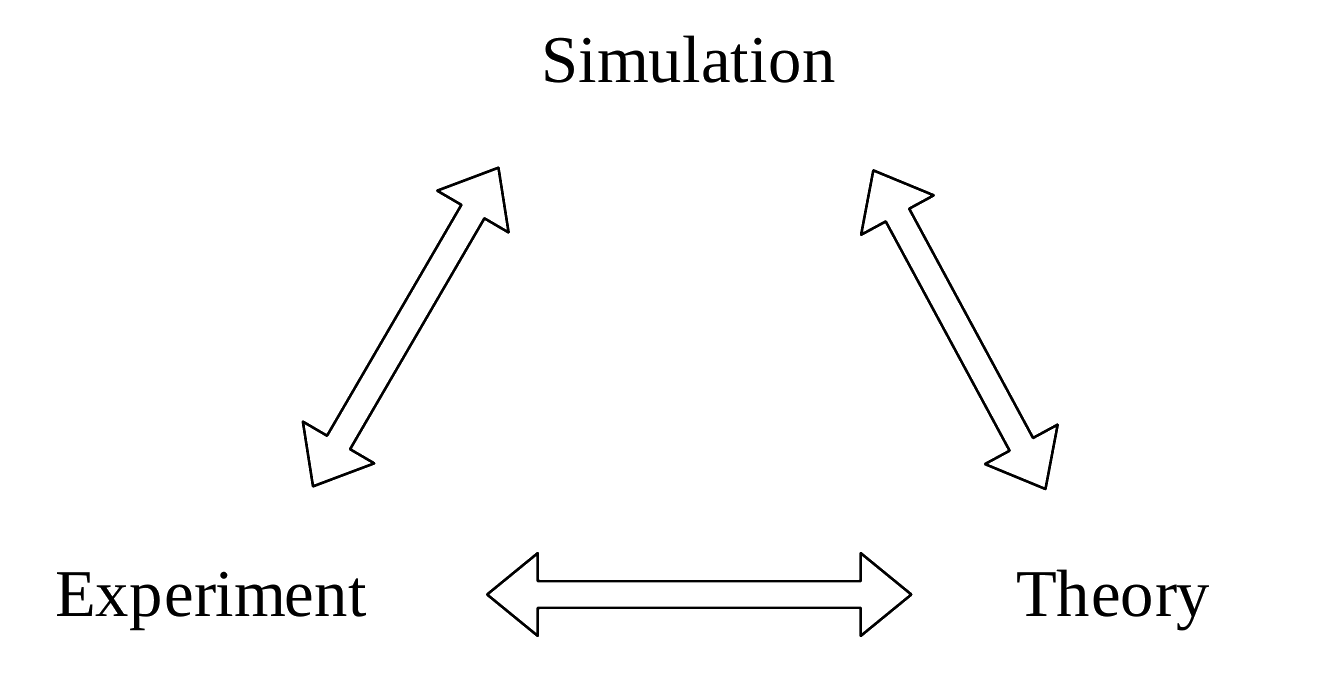
\includegraphics[width=0.7\textwidth]{images/ResearchTriangle.png}
        \caption[Research Triangle]{The research 
triangle showing the synergy between theory, experiment and simulation.}
        \label{fig:1}
\end{figure}

The least expensive method is geometry optimization in which the energies and geometries of the 
system energy minima or saddle points are obtained by an optimization procedure. This method 
has the limitations of only sampling states close to the initial configuration, which can be 
troublesome in complex potential energy surfaces, and it models entropic and solvent effects 
in a crude fashion\cite{Cramer2004_v2}. In contrast,  Monte Carlo or Molecular Dynamics 
(\gls{md})
methods do Boltzmann sampling of -ideally- the full configuration or phase space and includes 
solvent and 
entropic effects explicitly. Monte Carlo simulations sample stochastically configuration space 
by making random moves in the system and accepting them into the statistics with a probability 
based on their Boltzmann weight\cite{frenkel2001understanding}. MD is based on 
the propagation of the equations of motion of the system and the resulting trajectory is 
analyzed. MD is theoretically founded on the ergodic hypothesis which states 
that ensemble average properties are equal to time averages properties if the phase space is 
sampled fully.\cite{Smith2014} In many cases this hypothesis is a reasonable assumption, but in 
cases with high free energy barriers between relevant states the trajectory might 
be stuck in one of the states and not sample the other. To have access to these states within 
the MD simulation approach, enhanced sampling methods like 
metadynamics (\gls{metad})\cite{Valsson2016,bussi2015free} can be used. In enhanced sampling 
methods 
a bias potential is added to the simulation hamiltonian in order to force sampling in the 
relevant states of the system. The extra complexity of enhanced sampling simulations is 
rewarded with the generation of a free energy surface of the system. Finally, in order to 
calculate the free energy difference between different chemical systems free energy 
perturbation methods can be used\cite{Shirts2013_v2}. 





\section{Metal Ion Force Fields}\label{sec:MIFF}

Ions in solution are among the first systems to be studied with MD. 
The reason being that there is no question about their importance. They 
are present in all natural waters, in an enormous part of industrial processes, and are crucial to 
biochemistry (one third of pdb protein structures contain metal ions\cite{solomon1996volume}).

The first simulation of ions in water was performed by Heinzinger and Vogel over 50 years 
ago studying aqueous LiCl\cite{heinzinger1974molecular}. They modeled water with the ST2 model of 
Rahman and Stillinger\cite{rahman1971molecular} and obtaining van der Waals parameters for the 
ions from their iso-electronic noble gas parameters of 
Hogervost\cite{hogervorst1971transport}. Despite the simulation capabilities of the time, the 
simulations showed good agreement between the first-shell properties and X-Ray diffraction 
experimental data. Furthermore, they predicted the faster rotation time of the 
first-shell water molecules with respect to bulk in agreement with \gls{nmr} data. Other 
pioneers 
and 
front-runners in this research were Jorgensen et 
al.\cite{jorgensen1982quantum,chandrasekhar1984energy,jorgensen1983comparison}
and $\AA{}$qvist\cite{aqvist1990ion}  in the eighties and nineties respectively.  

The most common feature across popular aqueous ion force fields is their functional 
form:

\begin{equation}\label{eqLJ}
E_\text{int}=
\sum_{i=1}^N\sum_{j>i}^N 
\frac{q_iq_j}{4\pi\epsilon_0 r_{ij}}+ 
\sum_{i=1}^N\sum_{j>i}^N
4\epsilon_{ij}\left[\left(\frac{\sigma_{ij}}{r_{ij}}\right)^{12}-\left(\frac{\sigma_{ij}}{r_{ij}}
\right)^6\right]
\end{equation}

Where $E_\text{int}$ is the interaction energy between all the particle pairs $i j$. We shall 
not 
discuss the water force field which has been reviewed 
elsewhere\cite{PhysChemChemPhys_Vega_2011}. Many other functional forms exist: 
Born-Mayer, Mie, Morse etc.\cite{Li2017} Nevertheless, the one presented above is the most 
representative in the literature.  

The first term of the equation is the electrostatic term which features the integer charge 
of the ion and the partial charges of the water model. This term is generally evaluated using an 
Ewald sum variant\cite{frenkel2001understanding}. We neglect two effects in this force field 
approach: charge transfer to the 
first shell and polarization of the water molecules. They 
cannot be represented explicitly within the pair interaction approximation: all forces depend 
on the atom pair relative positions. This makes the force calculation algorithm 
computationally fast. Charge transfer and polarization are intrinsically many-body effects and 
not pair interaction effects. Modelling charge transfer and polarization in pair 
potentials remains one of the key parts of ion interaction potential development. Force fields 
which include many-body effects in pair potentials are know as \textit{effective pair potentials}.

The second summation of Equation \ref{eqLJ} is the van der Waals interaction between 
the atom pairs. In ion-water interactions they are less important in magnitude than 
electrostatics but crucial to the modelling. In Equation \ref{eqLJ} this molecular interaction 
is described by the Lennard-Jones function.



Lennard-Jones based force fields have proven to be fairly robust in treating monovalent ions 
in a simple and inexpensive fashion. But, their performance degrades heavily on multiply-charged 
cations or molecular cations\cite{Li2017,Li2015,Li2013}. This is a consequence of 
the increasing weight of charge transfer and polarization as the cation charge increases. This 
is the Achilles' heal of Lennard-Jones potentials.


Regardless of its functional form, the parameters of the force field are fit with respect to 
experimental data (empirical force fields) and/or \textit{ab initio} calculations (\textit{ab 
initio} force fields). In cation force fields the $q_i$ are 
given by the water model and the charge of the ion in particular. Only the Lennard-Jones 
parameters remain to be fit. 

If the fitting is done with respect to empirical data, the force field guarantees that 
properties introduced in fitting data set are reproduced. It is reasonable to expect that 
properties that correlate with the fit data are fairly well reproduced too. Free energy of 
hydration and ion first-shell distance are an example of this\cite{Li2015}. Further 
extrapolation should be done with additional skepticism. 

\begin{figure}
     \centering
         \includegraphics[width=\textwidth]{images/E_int.png} 
        \caption[Many body effects in the Po(VI) hydrate.]{QM interaction energies of 
\ce{[Po(H2O)_n]^{4+}(g)} per water molecule as a function of n at the MP2 level of 
theory.\cite{Ayala2008} This example illustrates how the interaction energy of a highly charged 
cation with its first shell water molecules is a many-body interaction. If this was not the case, 
a horizontal line would be obtained.}
        \label{PoEint}
\end{figure}

\textit{Ab initio} force fields are parametrized with respect to energies and molecular 
structures obtained from quantum chemistry calculations. This strategy has several advantages. 
If the sampling of the system potential energy surface is exhaustive enough and at a 
reasonable level of theory, the prediction of information for which the force field was not 
specifically designed is 
typically better than using empirical force fields. In addition, the fitting data sets can be 
generated easily. Especially since medium-level calculations produce satisfactory results in 
most properties. This is particularly appreciated in experimentally challenging 
systems like radioactive elements. \textit{Ab initio} force fields have a clear improvement 
path; just add more structures or improve the level of theory. For these reasons the 
interaction potentials developed in this thesis will all be classical force fields based on 
\textit{ab initio} calculations.

The traditional strategy to obtain the QM data is to calculate the 
interaction energies of the monohydrate, \ce{M^{+n}}-\ce{H2O}, at different metal oxygen 
distances. This has two shortcomings for highly charged cations. 

\begin{figure}
     \centering
         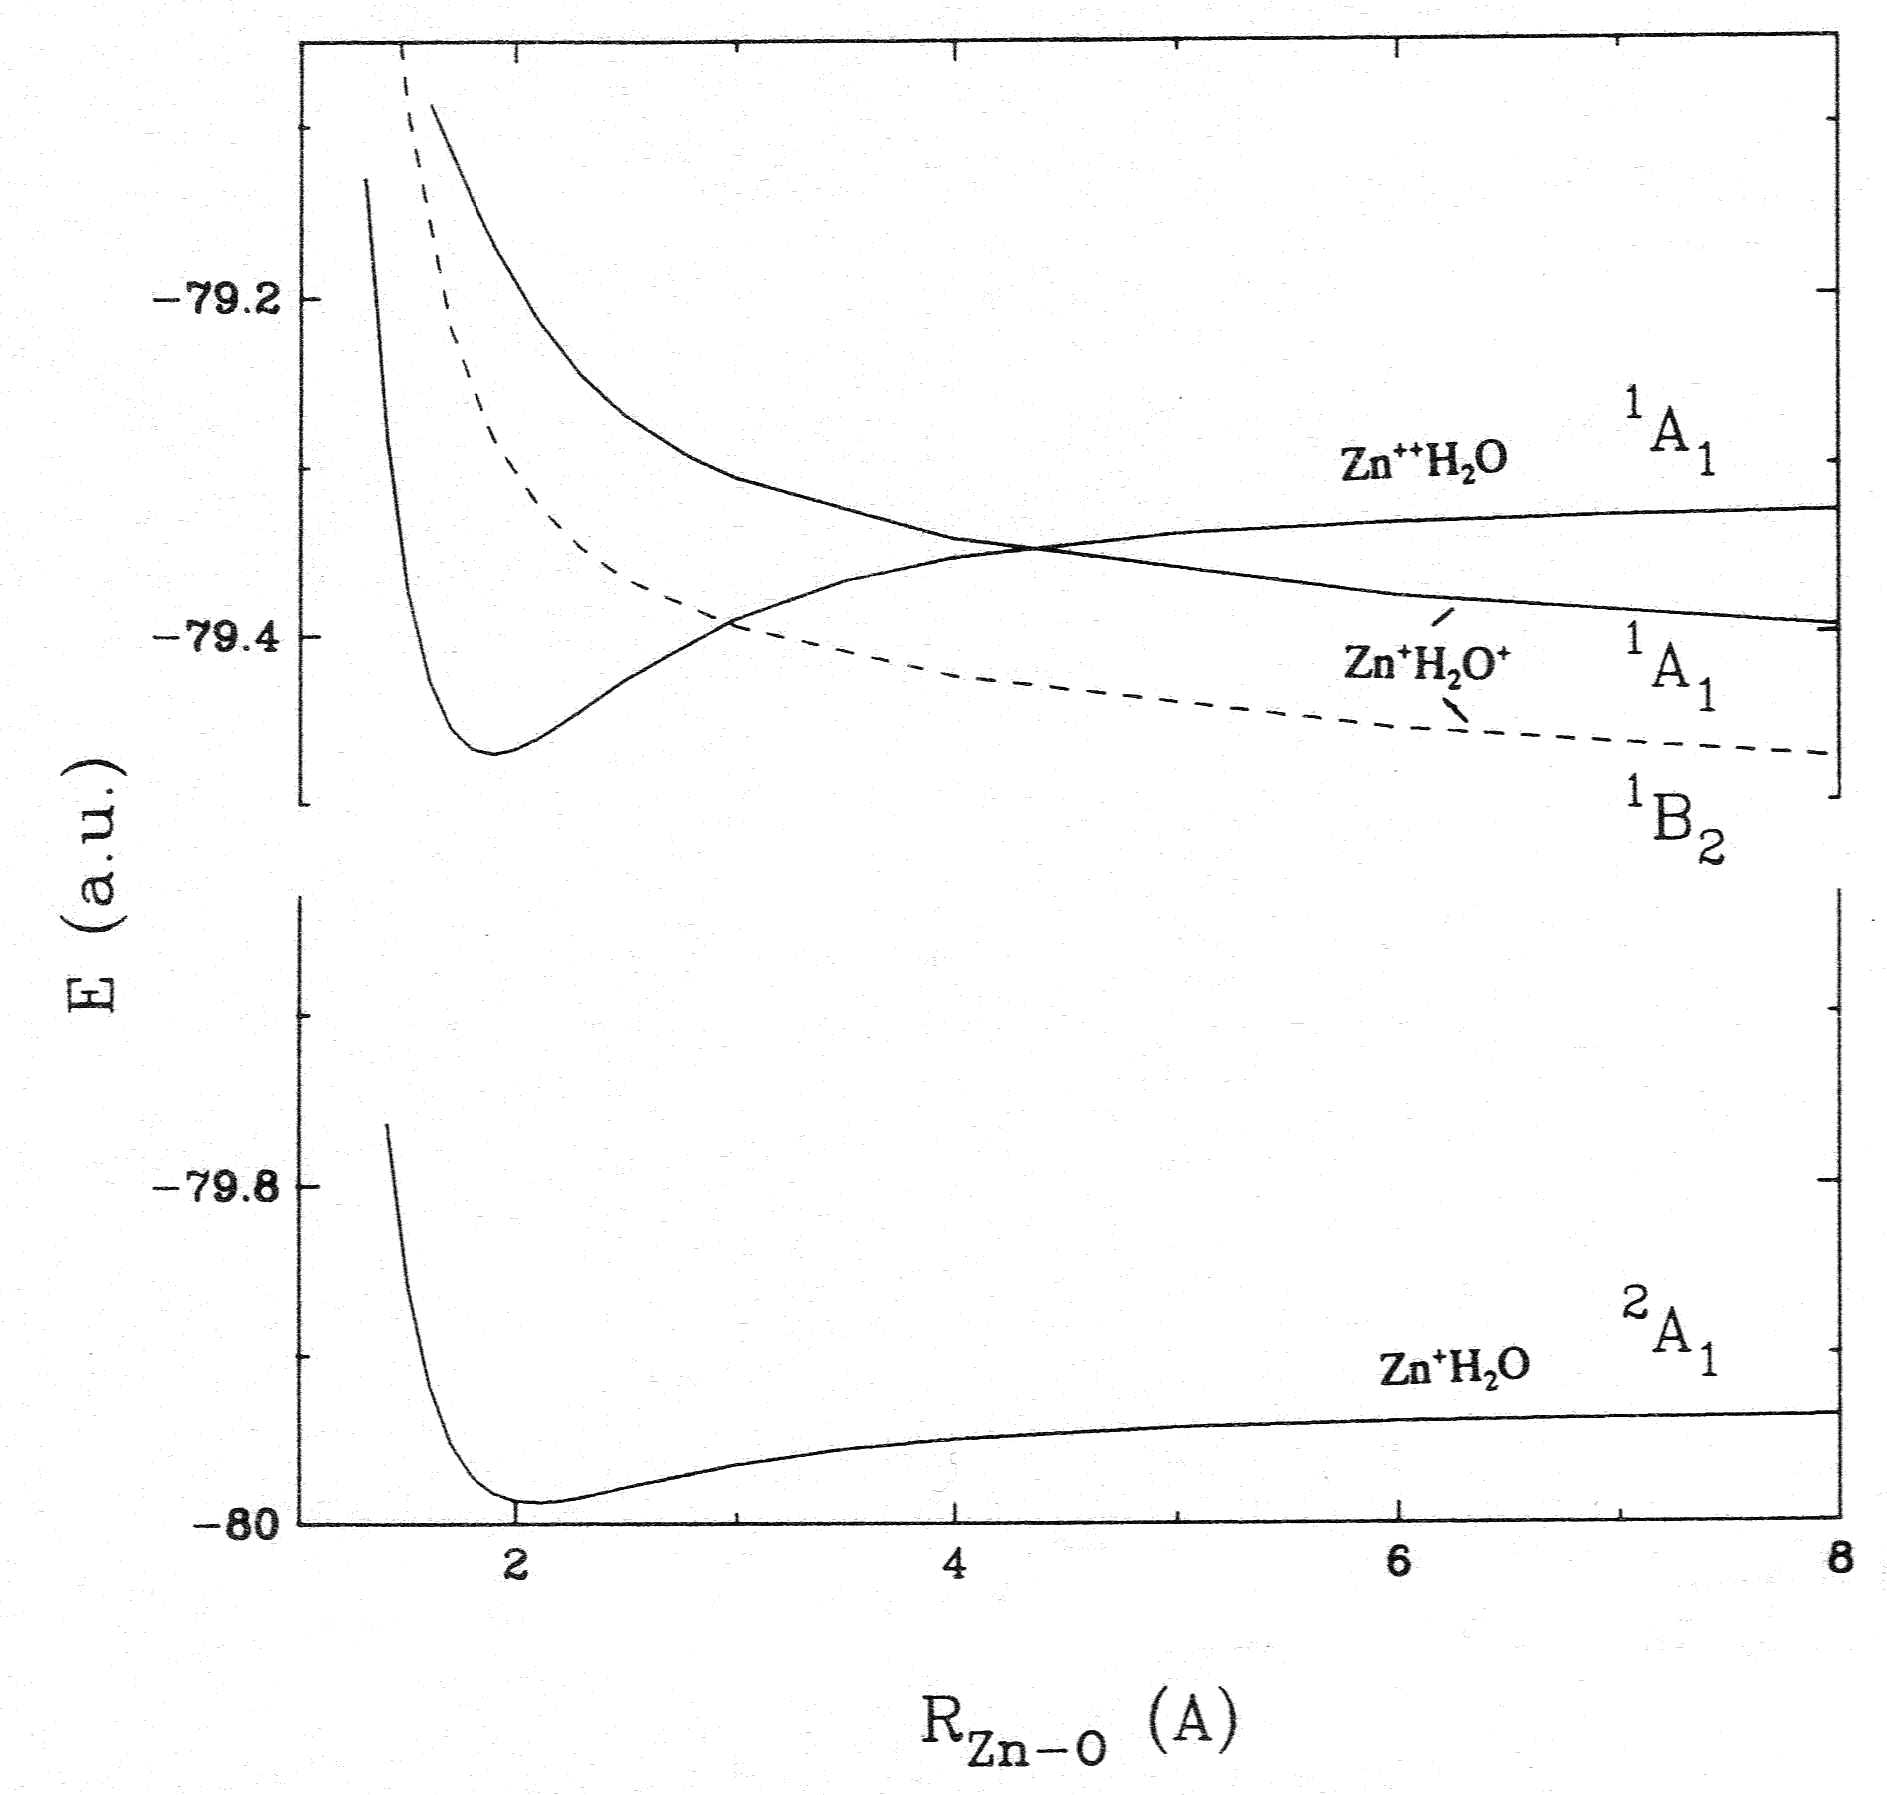
\includegraphics[width=0.7\textwidth]{images/ZnQM} 
        \caption[Charge transfer in \ce{[Zn*(H2O)]^{2+}}]{Hartree Fock energies for the ground 
state 
of  \ce{[Zn*(H2O)]^{+}} ($^2A_1$) and 
\ce{[Zn*(H2O)]^{2+}]} lowest states ($^1A_1$ and $^1B_2$). For the monovalent there are no low 
lying excited states but for the divalent there are two charge transfer states which are the lowest 
in energy at long distances. Reproduced with permission of the 
authors\cite{JPhysChem_ESM_1992}.}
        \label{ZnQM}
\end{figure}

The first is that the average total hydration enthalpy is highly overestimated. The cause of 
this is that the interaction energy in the monohydrate is much more 
negative than the interaction energy of the individual water molecules around an ion when 
fully solvated. In other words, the interaction energy of the metal with its first shell 
is different from the interaction energy of the monohydrate times the coordination number. 
This is because when going from the monohydrate to the n-hydrate the polarizing 
capability per water molecule of the ion decreases with n. The 
interaction energy per water molecule decreases as you increase the number of molecules in the 
first shell as is illustrated in Figure \ref{PoEint}. This means that the interaction energy of 
a cation with its 
first shell is a many-body case (in this case a ``body'' refers to a water molecule). In 
addition, 
the water-water repulsion in the fully-hydrated ion lengthens the M-O distance decreasing the 
interaction energy. These effects are impossible to capture with monohydrate based 
potentials.\cite{curtiss1987nonadditivity,JPhysChemA_ESM_2000}

The second problem of monohydrate potentials is that, for highly charged cations, when scanning 
quantum mechanically the 
M-\ce{OH2} distance there can be electronic state crossings that lead to a charge transfer 
state. This is
shown in Figure \ref{ZnQM} for the \ce{[Zn*(H2O)]^{2+}]} case. The reason for this is that 
ionization potential of water is lower than the second ionization potential of 
Zn(g) but not of Zn(aq).\cite{floris1995free,JPhysChem_ESM_1992} This behavior has also been found 
in other 
metals like \ce{Be^{2+}} and 
\ce{Fe^{3+}}.\cite{JPhysChemA_ESM_2000,Elrod1994,curtiss1987nonadditivity}

Additionally, in the case of systems with unpaired electrons the electronic 
state of the ion is heavily influenced by the ligand field around it and the monohydrate cannot 
represent the fully hydrated ion. This is typical of most electronic states of transition 
metals and actinoids. The  coordination of a full solvation shell stabilizes the ground state 
making it less sensitive to 
geometrical distortions.

To alleviate many of these problems our group developed about 25 years ago the Hydrated Ion Model. 
In this thesis we present its last extensions to the actinoid cations and its integration into a 
mineral matrix, montmorillonite clay. 

\section{The Hydrated Ion Model}\label{sec:HIM}
The Hydrated Ion Model (\gls{him}) is a modelling strategy to develop cation interaction potentials. 
It is 
inspired by the classical electrochemical concept of the hydrated ion in which the hydrated ion, 
\ce{[M*(H2O)_m]^{n+}}, is the solute and active species in solution instead of the 
naked ion, \ce{M^{n+}}. In this 
way the hydrated ion becomes the solute and target of study. The ion and its first solvation shell 
are now considered an entity (a molecule) which has special water molecules inside and that is 
surrounded by 
different bulk water molecules. Traditionally, the picture was of a charged atom surrounded by bulk 
water molecules making no distinction between first and outer solvation shells. 

This conceptual change has several important implications. All 
QM calculations must be done with the HI, \ce{[M*(H2O)_m]^{n+}}. This inclusion of 
the full first shell has deep consequences on the interaction QM energies used to parametrize the 
interaction potential and therefore in its development. Since the full shell is present there is no 
over-polarization of  first-shell molecules like in monohydrate models. The interaction energies 
are similar to those in solution since the nearest-neighbor environment is the same. Many-body 
effects are explicitly included in the interaction energies and therefore implicitly incorporated 
in the force-field. Wavefunction related problems are 
avoided because the full shell stabilizes the electronic state with respect to electronic degeneracy 
and charge transfer dissociation limits. This feature is of great interest for high charge cations. 

\begin{figure}
\centering 
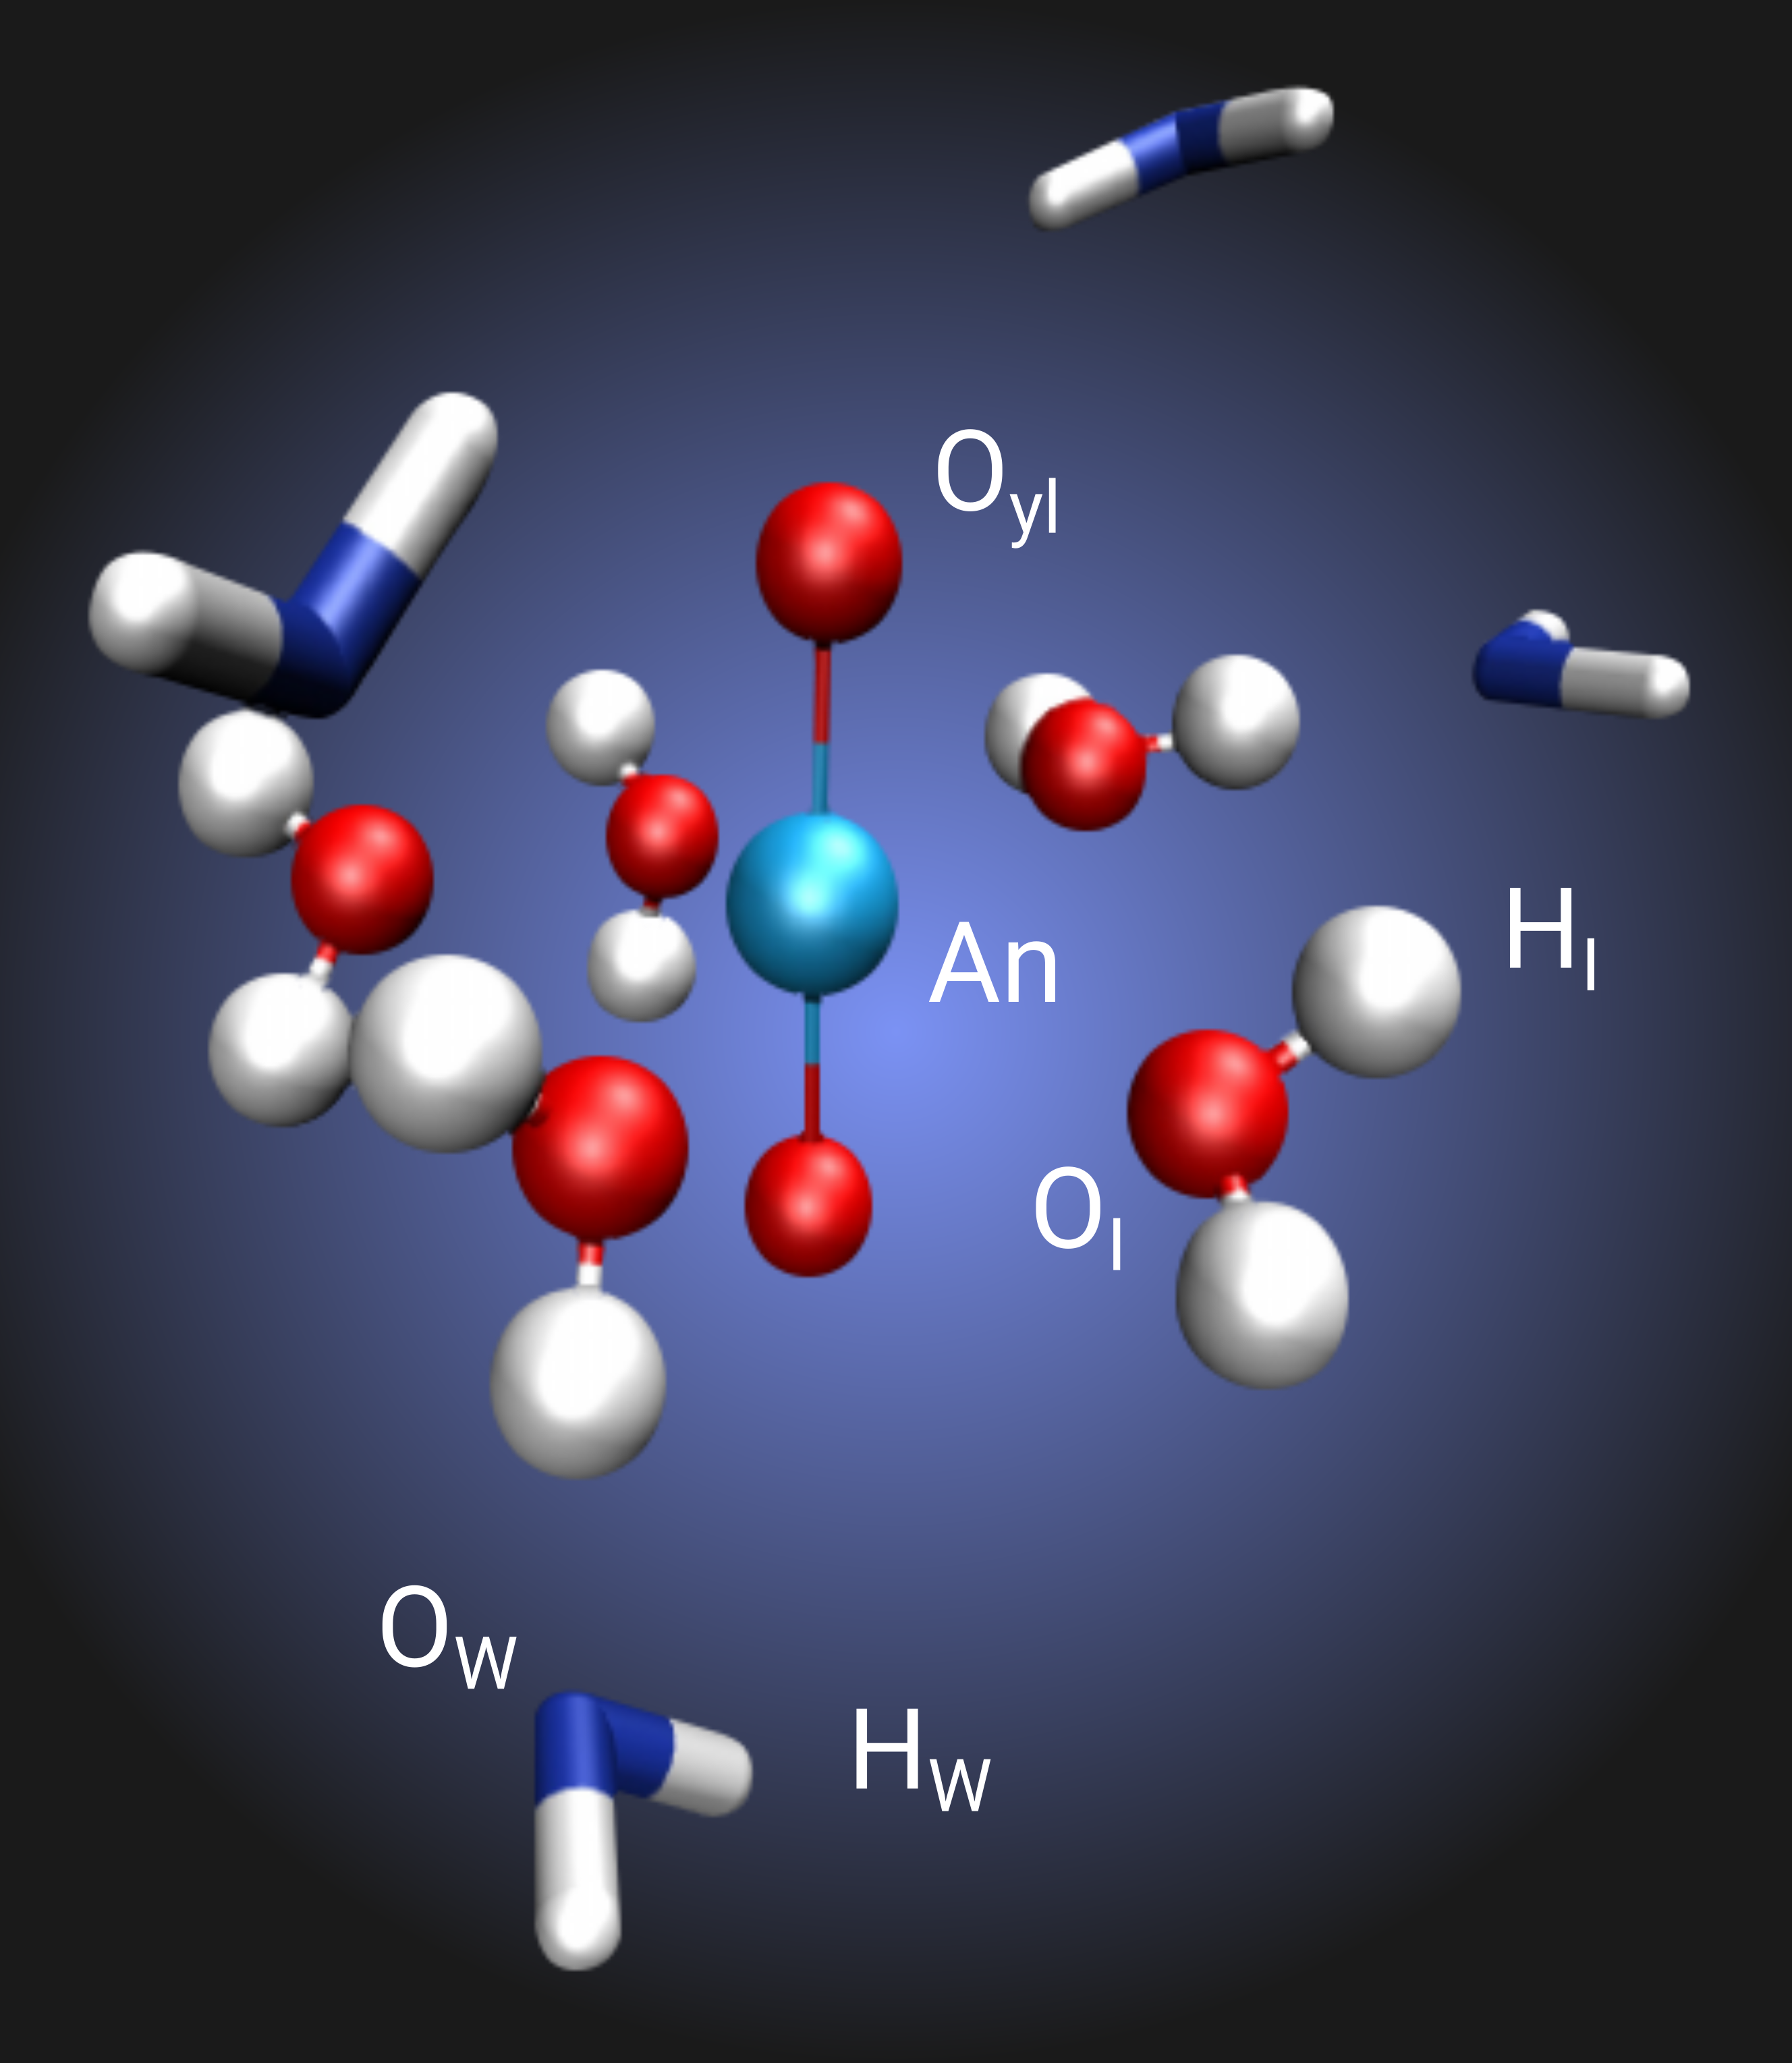
\includegraphics[width=8cm]{./images/HI_labels.png}
\caption[Hydrated ion atom types]{Image of an actinyl hydrated cation \ce{[An*(H2O)5]^{n+}} in 
water. Only some bulk water molecules are drawn for clarity. Bulk water molecules are drawn with 
the ``licorice'' representation and first-shell water molecules are represented with the ``ball and 
stick'' representation.}
\label{HI_labels}
\end{figure}

The considerations of the HI as the consistent molecular cation in solution allows us to assign 
different atom types (\ce{O_I} and 
\ce{H_I}) in first-shell water molecules than in the rest of bulk water molecules (\ce{O_W} 
and \ce{H_W}). Figure \ref{HI_labels} illustrates this. The HIM provides great flexibility to 
the 
potential 
because the bulk water molecules can 
be modeled with conventional classical force fields (TIP4P in our case) and first-shell water 
molecules can be given different 
geometries, partial charges and interaction potentials. The first-shell water molecules can now 
have 
a higher dipole than bulk water and even be charged due to partial charge transfer from the metal 
center. Assignment of these partial charges can be done with conventional partial charge 
calculation methods like CHELPG or RESP calculated on the full HI. Charge transfer and polarization 
of the first-shell and its differentiation from the bulk is a feature of great interest for 
high-charge cations since their first-shell is specially different to bulk.

This strategy of parametrization stems from considering in a more realistic way the nature of the 
ion. Unfortunately, there is a price to pay. The payment is done in terms of complexity of the 
potential. Fortunately, this increase in complexity is manageable. Two interaction potentials must 
be fit and therefore two potential energy surfaces must be scanned: the first-shell ion potential 
energy surface which governs intra-HI motion and another for the interaction of the HI with bulk 
water. In addition, to capture properly all the effects that can be accessed with this model,
the functional form of the force fields are typically complex. The functional forms used are 
a sum of $r^{-n}$ terms and an electrostatic term:
\begin{equation}
E=\sum_{i=1}^{\substack{\text{HI} \vspace{0.02cm}\\ \text{sites} }} 
\sum_{j>i}^{\substack{\text{water} \vspace{0.02cm}\\ \text{sites} } }
\left(\frac{C_{12}^{ij}}{r_{ij}^{12}}+\frac{C_{8}^{ij}}{r_{ij}^{8}}+
\frac{C_{6}^{ij}}{r_{ij}^{6}}+
\frac{C_{4}^{ij}}{r_{ij}^{4}}+
\frac{q_iq_j}{4\pi\epsilon_0 r_{ij}}\right)
\end{equation}
Because the number of coefficients is relatively high the 
potentials are more prone to over-fitting. In addition, combination rules with 
other atom types are impossible to use. This can hinder the recycling of potentials developed for 
particular systems to others, although generalizations have been 
done\cite{JACS_ESM_1999,Martinez2004,JPhysChemB_ESM_2007}. Another 
problem associated 
to the functional form is that most MD programs do not allow using this functional 
form in a simple way limiting its use to less specialized users. Nevertheless this leads to 
the development of potentials that have very high accuracy, in particular in properties 
depending on first and second hydration shells, that can reproduce subtle experimental 
properties such as EXAFS 
spectra\cite{Angew_ESM_2010,Merkling2001,JACS_ESM_2002,caralimpio2018looking,thesisNoe}.

The problem of having new atom types for first-shell water molecules is that if they leave the 
first shell and diffuse into the bulk the model becomes unphysical. Fortunately, for 
high-charge cations this is not a problem, it is a feature. Residence times of water molecules 
of most cations with charge greater than one have timescales much longer than the simulation 
time: any change in coordination or water exchange is unphysical anyway. The HIM considers the 
HI as the molecular cation in solution so the interaction between the first-shell water oxygen 
and the metal cation may be viewed as a flexible bond. Nevertheless, this interaction 
potential 
is not a harmonic function. The \ce{M-O_I} interaction goes to zero as $r \rightarrow \infty$. The 
water molecules, in principle, can leave the first shell but the barrier to do it is high 
enough 
to prevent it in the simulation timescale. If this event were to happen, the potential 
should 
be reexamined. An additional advantage of having such a flexible functional form in the \ce{M-O_I} 
interaction is that it captures anharmonicities of the bonding which an harmonic potential is 
unable of doing. 

In some cations with low charge/radius ratio, like heavy alkalines and lanthanoids, the water 
exchange 
and the changes in coordination number are frequent. The HIM can also be used to develop potentials 
for these systems but some modifications must be done. Only one type of water molecules must be 
used and in order to capture the polarization and many body effects a polarizable potential must 
be used\cite{caralimpio2018looking,thesisNoe,Angew_ESM_2010,JChemPhys_ESM_2015}. The price to pay 
for this extra flexibility of the 
potential is that the force field becomes more computationally demanding and charge transfer to the 
first shell is neglected, which should be residual anyway. This model is know as the exchangeable 
HIM. 

I will now briefly explain the historical development of the HIM across a good part of the periodic 
table. The HIM model started as solution to the problems found studying the potential energy 
surface of the \ce{Zn^{2+}} monohydrate\cite{JPhysChem_ESM_1992} therefore the first HI to be 
studied was \ce{[Zn*(H2O)6]^{2+}}.\cite{JPhysChem_ESM_1993} The HI was rigid and the parametrized 
interaction was the HI-bulk Water Interaction or $E_{HIW}$. The unprecedented  
agreement with the experimental hydration enthalpy obtained by Monte Carlo simulations  
revealed the robustness of the force field development strategy and encouraged its extension in 
a similar fashion to  \ce{[Cr*(H2O)6]^{3+}} with similar 
success\cite{JPhysChem_ESM_1996,JPhysChemB_ESM_1998}. The next 
step in the 
progression was to make the HI flexible by parametrizing its internal degrees of freedom with the 
Ion First-Shell Water potential, $E_{IW1}$. This was initially done for \ce{Cr^{3+}} but 
has become standard in the development of the HIM since.\cite{JChemPhys_ESM_1998} The great 
advantage of internal flexibility is that it allows power spectra calculation of the 
aqua ion and 
also the X-Ray Absorption Spectra which is a subtle experimental property to 
reproduce due to the high structural 
sensitivity\cite{Angew_ESM_2010,Merkling2001,JACS_ESM_2002,caralimpio2018looking,thesisNoe}. A 
variety of cations were also studied using this approach, 
\ce{Be^{2+}},\ce{Mg^{2+}},\ce{Al^{3+}},\ce{Rh^{3+}}, 
\ce{Ir^{3+}} and even \ce{Th^{4+}}.\cite{Martinez2004,JPhysChemB_ESM_2007,JACS_ESM_1999,Yang2001} 
This 
version of the HIM will be 
the one used to study actinyl pentahydrates in the thesis. The difference with previous versions is 
that the actinyl model will include an intramolecular cation interaction potential, 
$E_\text{IMC}$ which 
will define the dynamics within the actinyl unit (\ce{[AnO_2]^{2+}}). In this way we will deal with 
the fact that the cation will be molecular instead of atomic. 

Another set of cations studied using the HIM are the square planar noble metals dications, 
\ce{[M*(H2O)4]^{2+}}. The first two studied metals were \ce{[Pd*(H2O)4]^{2+}} and 
\ce{[Pt*(H2O)4]^{2+}} and its aquo-derivatives\cite{JPhysChemB_ESM_2004,Torrico2006}. A few 
years later the methodology was 
extended to study the chemotherapeutical 
cis-platin,\newline\ce{[PtCl2(NH3)2]^{2+}}.\cite{JChemTheoComp_ESM_2013,Melchior2015} The 
study of these 
compounds gave 
a picture of a single ion with two solvation environments: one equatorial that follows conventional 
solvation and a different axial solvation. This differentiated axial solvation was 
labeled the ``meso-shell'' since it is characterized by metal-ion distances in between the first 
and the second
shell, with orientations and lability resembling the second shell. This behavior 
of a single ion having two very different solvation regions will also be encountered in 
actinyls.

The last category of HIM ions are studied with a polarizable ion and water model, 
MCDHO and MCDHO2\cite{MCDHO,MCDHO2}. This allows the possibility for water exchanges in the 
first-shell and changes in coordination number. This model is known as the exchangeable HIM. The 
main advantage of this model is the ability to study cations with fast first-shell water exchange 
rates 
and varying coordination number. There have been numerous cations studied in this way: the 
alkalines, alkaline earth metals, several lanthanoids and actinoids, \ce{Sc^{3+}} and 
\ce{Tl^{+}}\cite{caralimpio2018looking,thesisNoe,Angew_ESM_2010,Caralampio2017b,Caralampio2017,
Morales2016,Yang2001}. These models allow theoretically predicting the coordination numbers in 
solution 
which is experimentally challenging in some cases like 
\ce{Sc^{3+}}.\cite{Caralampio2017b,cotton2018scandium}





\section{X-Ray Absorption Spectroscopy}\label{sec:XAS}
If a sample of thickness, $d$, and concentration, $c$, is irradiated by light-source of 
intensity, 
$I_0$, which transmits an intensity, $I$, we can characterize the absorbance of the sample by its 
absorption coefficient, $\mu$, according to the Lambert-Beer's Law:
\begin{equation}
 \mu=\frac{1}{c\cdot d}\ln{\frac{I_0}{I}}
\end{equation}
If the light source used is an X-Ray beam, the study of $\mu$ as a function of the photon 
energy is a technique known as X-Ray Absorption Spectroscopy (\gls{xas}). One of humankind's most 
important discoveries was based on XAS: Moseley's law. In 1913, Henry Moseley discovered that the 
square root of the lowest frequency line of the XAS spectrum of an atom was 
proportional to its nuclear charge. This discovery proved that an element's position in the 
periodic table is due to its nuclear charge and not its mass, consolidating Bohr's model of the 
atom as universal across the Periodic Table. 

Twenty years after Moseley's law, Kroning discovered that the XAS spectrum of condensed 
matter atoms had a fine structure that could in principle be related to the structure around 
the absorbing atom. XAS had to wait until the seventies to become the relevant 
chemical and structural characterization technique it is today. Sayers, Stern and Lytle in 
1971 discovered that through XAS one could have access to the pseudo radial 
distribution function of the absorbing atom with its neighboring atoms.\cite{sayers1971new} XAS has 
become widely 
available by the development of the 
intense synchrotron radiation sources used to measure the spectra. 

XAS is still one of the most important techniques of structural and chemical characterization 
particularly of disordered materials and metals in solution. It provides highly detailed and 
highly accurate information of the local structure around a particular atomic center and of 
its oxidation state. It has the additional advantage that it is element specific. It can be 
used in very dilute conditions ( $10^{-4}$\si{\molar} ) becoming suitable for the study of 
highly radiotoxic elements like plutonium.

When increasing the energy of the incident X-Ray beam the absorption is low until at 
a certain energy value $\mu$ suddenly increases. At this point, the X-Ray photon has 
the exact energy as the ionization energy of one of the atom's core-electron, the photon is 
absorbed 
and the atom is ionized. This absorption jump is known as absorption edge. The absorption edge is 
element-specific and the absorbing atom is typically chosen to be the metal center. In addition, 
different core 
electrons can be ionized. This generates different edges of the element which are 
labeled by the principal quantum number of the ejected photoelectron ($n=1 \rightarrow 
K$,$n=2\rightarrow L$ 
etc). 

If the absorbing atom is a monoatomic gas, increasing the energy of the 
photon beyond the edge causes the emission of the photoelectron with additional kinetic 
energy. This results in a monotonic decay of $\mu$. If the absorbing atom 
is in a condensed phase the decrease in absorption is not monotonic but 
rather presents an oscillatory fine structure. The study of this fine structure is the basis 
of chemical and structural characterization using XAS. This oscillatory behavior depends on the 
nature of the atom and the interaction of the ejected photoelecton with the electronic density of 
the nearest neighbors of the atom. The ejected photoelectron can be backscattered by the
atoms surrounding the absorber doing a round trip out of the absorber and back. The 
constructive or destructive interference of the outgoing and ongoing photoelectron wavefunctions 
increases or decreases the probability of ionization generating the oscillatory 
behavior in $\mu$. This effect is a consequence of the particle-wave duality of electrons. 

The interference pattern is a function of the kinetic energy of the electron, the distance to the 
neighbors and its thermal fluctuation, the coordination number and other spectroscopical factors. 
Modelling this interference is the 
aim of XAS interpretation. 

\begin{figure}[h!]
\centering
\includegraphics[width=9.2cm]{./images/XAS.png}
\caption[X-Ray Absorption Spectrum]{ Sr
L-edge X-Ray 
absorption spectrum in \ce{SrCO3(s)}. The data was obtained from the XAFS spectra library of 
the University of Chicago. 
\SI{7120}{\electronvolt}-\SI{7220}{\electronvolt} region corresponds to 
XANES and \SI{7220}{\electronvolt}-\SI{7790}{\electronvolt} region to EXAFS. }\label{xas}
\end{figure}

Figure \ref{xas} shows a XAS spectrum of Sr in \ce{SrCO3(s)}. The spectrum can be divided 
in 
two distinct regions:
\begin{itemize}
 \item \textbf{\gls{xanes}}: X-ray Absorption Near Edge Structure region of the spectrum. It 
extends from the absorption edge up to 100-\SI{150}{\kilo\electronvolt}. The 
photoelectron has little energy and multiple scattering processes are dominant. Quantitative 
analysis of XANES spectra is cumbersome due to multi-atom correlations and the complexity of the 
electronic problem itself. It is generally interpreted qualitatively. The position of the edge
itself is an indicator of the absorber oxidation state. Its shape is sensible to the 
symmetry of the environment and is regarded as a fingerprint of the local structure. 
\item \textbf{\gls{exafs}}: Extended 
X-ray Absorption Fine Structure region of the spectrum. It 
extends from $\sim$\SI{150}{\electronvolt} to $\sim$\SI{1000}{\electronvolt} above the 
absorption edge. Since the photoelectron has higher kinetic energy, simple backscattering paths 
dominate. This region contains most of the structural information: bond distances, coordination 
numbers and dynamic and structural disorder, that can be extracted by the use of the EXAFS 
equation. 
\end{itemize}

\begin{figure}
\centering 
\includegraphics[width=10cm]{./images/EXAFS.png}
\label{EXAFS1}
\caption[Uranyl EXAFS spectrum]{\ce{[UO2*(H2O)5]^{2+}} (blue) and \ce{[NpO2*(H2O)5]^{2+}} (orange)
L$_{\text{III}}$-edge 
k$^3$-weighted experimental EXAFS spectra.}
\label{EXAFS}
\end{figure}

\subsection{EXAFS Spectroscopy}

Above the absorption edge the absorption coefficient, $\mu$, follows the 
equation:
\begin{equation}
\mu(E)=\mu_0(E)[1+\chi(E)]
\end{equation}
Where $\mu_0(E)$ is the absorption coefficient of the gaseous monoatomic element and $\chi(E)$ is 
the 
fine structure function or EXAFS function or simply EXAFS spectrum. $\chi(E)$ contains the 
oscillatory fine structure of the spectrum resulting from the constructive and destructive 
interference of the photoelectrons backscattering paths. The EXAFS function is written with respect 
to the wavenumber of the photoelectron, $k$:
\begin{equation}
 k=\sqrt{2m_e(E-E_0)}/\hslash
\end{equation}
Where $m_e$ is the mass of the electron, $E$ the photon energy and $E_0$ the binding energy 
(or work function). Figure \ref{EXAFS} contains examples of experimental EXAFS 
spectra. The spectrum is typically weighted by $k^2$ or $k^3$ to emphasize the 
oscillations at high $k$ values.

The EXAFS equation can be written as\cite{sayers1971new}:
\begin{equation}\label{exafs}
\chi(k)=\sum_j^{\substack{\text{path} \vspace{0.02cm}\\ \text{types} 
}}\frac{N_j}{kR_j^2}\,\,S_0^2\,\,F_j(k)\,\,\eu^{\frac{-2R_j}{\lambda(k)}}\,\,\eu^{ 
-2\sigma_j^2k^2}\,\,
\text{sen}[2kR_j+\varphi_j(k)]
\end{equation}
The function is the sum of the terms of the different path types. The path types are all 
possible closed paths that go from the absorbing atom, to one or more backscattering atoms and back 
to the absorber including some that go several times through the absorber. If the path 
has only 
``two legs'', a round trip to a neighbor, it is considered a single scattering path (\gls{ss}). 
If the 
path has more than two legs, it is considered a multiple scattering path (\gls{ms}). Figure 
\ref{MS_SS} 
illustrates the kinds of paths observed.  In most cases  paths (round trips to a neighbor) 
dominate. 

\begin{figure}
\centering 
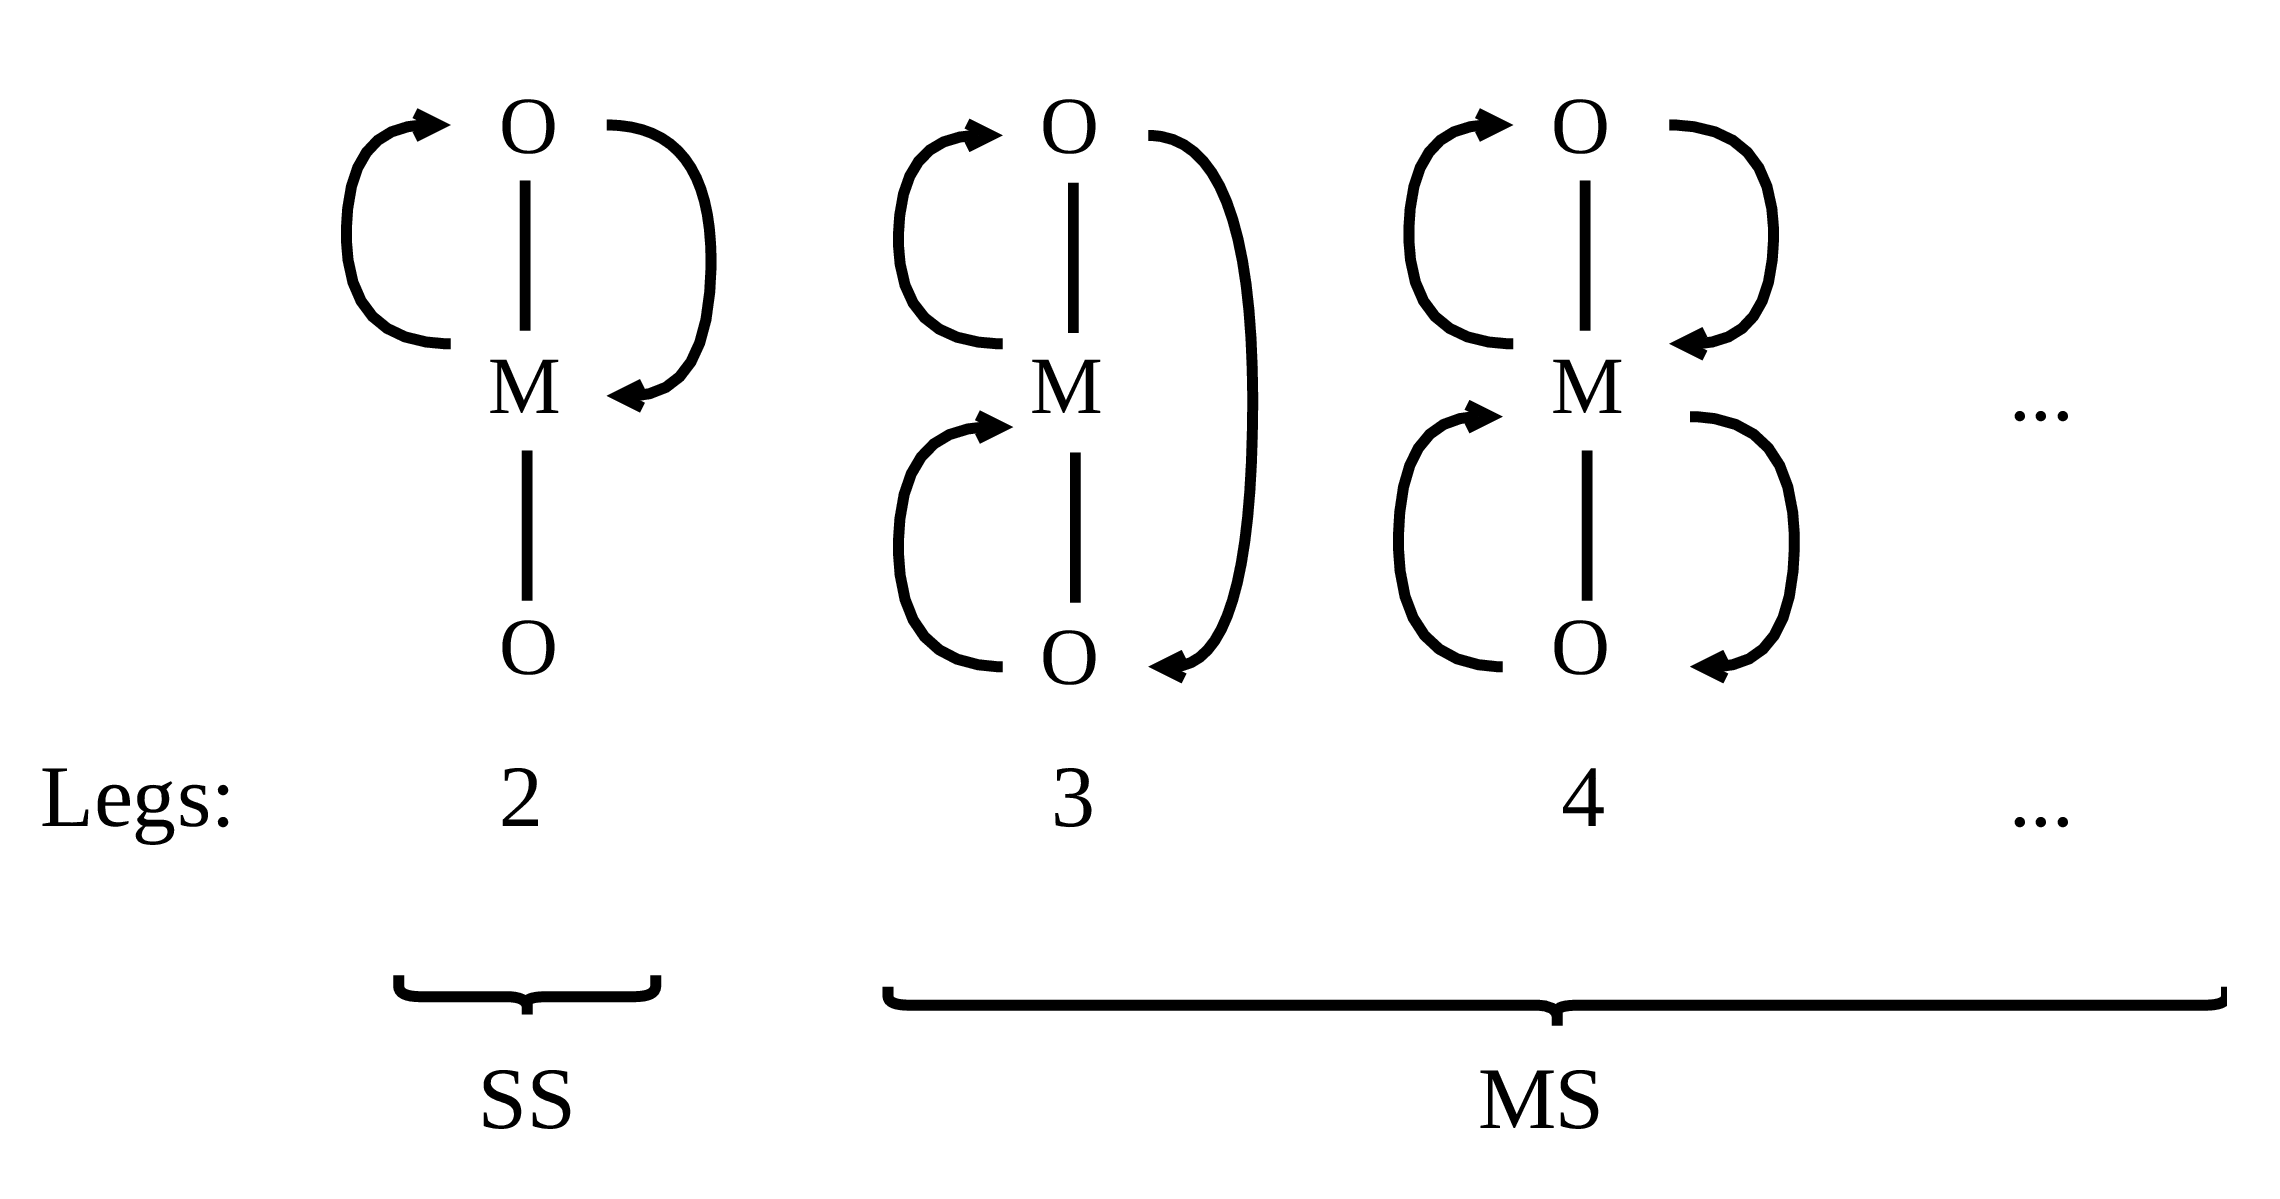
\includegraphics[width=10cm]{./images/Paths_diagram.png}
\caption[EXAFS paths illustration]{Examples of single scattering paths (\gls{ss}) and multiple scattering 
paths 
(\gls{ms}) with different number of legs. The absorber atom is M and the backscatterers are O. The 
arrows 
represent the paths the photoelectron travels.}
\label{MS_SS}
\end{figure}

The Fourier Transform of $\chi(k)$ is a pseudo-radial distribution function of the absorbing atom 
respect to its neighbor shells. It is not a true radial distribution function because multiple 
scattering paths do not depend solely on the absorber-backscatterer distance. 

First we will discuss the non-structural terms of Equation \ref{exafs} which are defined 
\textit{a priori} 
by the user or are estimated quantum-mechanically with  theoretical spectroscopy packages such 
as FEFF\cite{FEFF_PhysRevB_Rehr_2003,FEFF2_RevModPhys_Rehr_2000}.
\begin{itemize}
 \item The amplitude reduction function, $S_0^2$: It is a consequence of the 
fact that the electrons of the ionized atom experience a different potential than before the 
ionization and their wavefunction must relax to the ionized state. This factor must be included 
since only the electron and the neutral atom with a core-hole are modeled. It is typically assumed 
to have values from 0.85 to 1.0 but can also be estimated theoretically.
 \item Effective amplitude function of the path, $F_j(k)$: It has a complicated dependency on $k$ 
but it is determined by the atomic number of the backscattering atoms which serves as an
identification method for the local environment.
 \item Mean free path of the photoelectron, $\lambda(k)$: The method assumes that the wavefunction 
of 
the 
outgoing and backscattered photoelectron are coherent. This is only true during the life-time of 
the excited atom's core-hole. The method also assumes inelastic scattering. The factor $\eu^{ 
-2R_j/\lambda(k)}$ accounts for these two assumptions.
 \item Phase displacement function, $\varphi_j(k)$: Like $F_j(k)$, it has a complicated dependency 
on 
$k$ but it is determined by the atomic number of the backscattering atoms which serves as an
identification method for the local environment.
\end{itemize}
All these parameters can be nowadays calculated \textit{ab initio} by the FEFF program based on 
approximate 
relativistic quantum-mechanical self-consistent field calculations.

Now we will discuss the equation parameters that contain the structural information:
\begin{itemize}
 \item The distances to the backscattering atom, $R_j$: Actually, it is the path distance but for 
single scattering processes it coincides with the distance to the backscattering neighbor atom. 
$R_j$ control the frequency of the spectrum. Therefore, for systems with a single 
type of backscattering atoms and in the absence of significant multiple scattering contributions, 
the higher the frequency of $\chi (k)$ the longer the bondlength.
 \item The coordination number, $N_j$: Again, it is actually the degeneracy of the path but in 
single scattering processes it is equivalent to the coordination number. 
 \item The Debye-Waller Factor, $\sigma_j^2$: this parameter is the variance of the distance $R_j$ 
and measures the thermal dispersion or disorder of the path. The factor 
$\eu^{-2\sigma_j^2k^2}$ controls the envelop of the function and is responsible for the 
exponential 
decay of the fine structure. Therefore, a slowly decaying signal is associated with stiff 
structures, 
a small dispersion of path lengths and low Debye-Waller factors.
\end{itemize}

There are two ways of obtaining structural information out of an experimental EXAFS spectrum. One 
is pure experimental fitting. The spectrum is fitted to Equation \ref{exafs} with  
$\left\{R_j,N_j,\sigma_j^2\right\}$ as variables. If the spectrum has many non-equivalent 
backscattering atoms or complex features, the fitting process can be involved. In many cases, some 
of the parameters are fixed. These fixed parameters are obtained  from other experiments,
from theoretical studies or from educated guesses. This alleviates the burden of the 
high dimensionality of the problem. This fitting approach is particularly complicated in actinoids 
since there is little available experimental information for many of them so analogy with other 
actinoids is used in many cases\cite{coorchemrev_Denecke_2005}. 

In general, it is particularly difficult to fit 
with high precision the Debye-Waller factors and the coordination numbers since they are 
highly correlated. This is the reason why experimental coordination numbers obtained from EXAFS can 
have uncertainties of $\pm1$, while uncertainty in distances is much lower ($\sim\pm2\%$)

The combination of theoretical information with experimental spectra is another strategy to extract 
structural information 
from EXAFS. From the atomic positions of the absorbing atom and its nearest shells the FEFF program 
can calculate a theoretical EXAFS spectrum. If the theoretical and experimental spectra are in good 
agreement, the structural parameters of the theoretical coordinates are validated and proposed to 
characterize the system. Theoretical modelling of EXAFS is a great tool to interpret spectra, 
extract structural parameters, aid in the fitting and as a validation 
tool for newly developed theoretical models. In particular, computation of theoretical EXAFS 
spectra from statistical simulation ensembles can contribute to the interpretation of 
the experimental spectra\cite{Angew_ESM_2010,Dangelo_InorgChem_2013,spezia2017development,
ChemPhysLet_Filipponi_1994,JPhysChem_Palmer_1996,JACS_ESM_2002}. Conversely, reproducing the EXAFS 
spectrum helps to validate the quality of the simulation and the physicochemical predictions 
obtained. 

If the theoretical spectrum is calculated from a single molecular structure the Debye-Waller 
factors of the paths must be guessed since a single snapshot has no dynamic bond dispersion. 
On 
the other 
hand, if instead of a single structure we use an statistical simulation ensemble the path 
length 
dispersion is added explicitly from the statistical thermal fluctuation. The 
exponential decay term containing $\sigma_j^2$ is dropped from Equation \ref{exafs} and the 
theoretical EXAFS equation 
becomes:\cite{Merkling2001}
\begin{equation}\label{exafs-MD}
\chi(k)=\frac{1}{N_{s}}\sum_i^{N_{s}}\sum_j\frac{N_j}{kR_j^2}\,\,
S_0^2\,\,|F_j(k)|\,\,\eu^{\frac{-2R_j}{\lambda}}\text{sen}[2kR_j+\varphi_j(k)]
\end{equation}
The final spectrum is the average spectrum of the set of $N_s$ snapshots. The natural disorder 
introduced by the differences among  
the individual simulated spectra produces the exponential decay of the average function.

Both applications of the theoretical-experimental combination were done in this thesis. We used the 
theoretical EXAFS of an \ce{Am^{3+}}/\ce{[AmO2*(H2O)5]^{2+}} mixture to interpret its experimental 
EXAFS spectrum and predict the structural parameters of a pure \ce{[AmO2*(H2O)5]^{2+}} solution, a 
solution that experimentalists have been unable to produce so far.  We also used experimental EXAFS 
spectra to assess 
the quality of the actinyl force fields developed. 

More 
information of XAS spectroscopy 
can be obtained from the following 
review articles and monographs\cite{FEFF2_RevModPhys_Rehr_2000,JPhysChem_Palmer_1996,EXAFSreview, 
newville2004fundamentals,XASBook_Koningsberger_1988,AdelaCIC_v2}
. 


\section{Entropy In Molecular Dynamics Simulations}
As we have argued in Section \ref{sec:hydrophobicity}, entropy is one of the key factors in the 
hydrophobicity or 
hydrophilicity of a solute. 
Unfortunately, measuring entropic effects in simulation is a complex task. It generally involves 
either measuring the variation of free energy with temperature, $\left(\frac{\partial 
G}{\partial T}\right)_P=-S$, or by mathematically estimating how a process affects the number of 
microstates of 
a system. An example of the latter is tetrahedral entropy\cite{PNAS_Kumar_2009}.

Liquid state theory provides an additional path. The entropy of a system can be expanded as a 
sum of many-body 
correlations\cite{nettleton1958expression,baranyai1989direct}:
\begin{equation}\label{expansion}
S=S^{\left(1\right)}+S^{\left(2\right)}+S^{\left(3\right)}+\cdots
\end{equation}

This expansion has been used to study pure  
water\cite{Lazaridis1996,zielkiewicz2008two,Giuffre2010,Agarwal2011,Zhang2011} and solutions of 
simple 
solutes\cite{lazaridis1992entropy,lazaridis1994simulation,bergman1999topological,
lazaridis2000solvent,
kinoshita2006pair,liu2015order}. The use of the pair entropy expansion to calculate solvation 
entropies and 
free energies was formalized by Lazaridis in what is now commonly known as ``Inhomogeneous 
Solvation 
Theory'' 
(\gls{ist})\cite{lazaridis1998inhomogeneous}. Derivatives of this theory have been used to calculate the 
thermodynamics of structural water molecules of proteins\cite{li2012computing,Abel2008} or more 
complex solutes like amino-acids\cite{Nguyen2012,Huggins2013,Schauperl2016}

We will first assume that the system consists of a single spherically symmetric solute immersed in 
a rigid solute like the TIP4P\cite{TIP4P_JChemPhys_Jorgensen_1983} or 
SPC/E\cite{SPCE_JPhysChem_Berendsen_1987} water models.


In Equation \ref{expansion}, $S^{(1)}$  is the self correlation term, $S^{(2)}$  is the pair 
correlation term, $S^{(3)}$  
is the three-body correlation term, etc. Although the three-body term is expected to be 
significant, 
most of the information of the structure of the solution is in the pair 
term\cite{Lazaridis1996,nettleton1958expression,baranyai1989direct,wallace1987role}. 

The first order term, $S^{\left(1\right)}$, is the translational entropy of a non-interacting 
system: 
\begin{equation}
S^{\left(1\right)}=5k_\text{B}-k_\text{B}\ln 
\left(\rho_\text{s}\lambda_\text{s}^3\right)-k_\text{B}\ln\left(\rho_\text{w}\lambda_\text{w}
^3\right)
\end{equation}
where $\rho$ and $\lambda$ are the numeric density  and  the 
thermal 
wavelength of the solute (s) or the solvent (w) \cite{Lazaridis1996}.

The pair entropy term can be divided into three components:
\begin{equation}
S=S^{\left(2\right)}_\text{ss}+S^{\left(2\right)}_\text{sw}+S^{\left(2\right)}_\text{ww}
\end{equation}
The first term is zero due to the infinite dilution of the solute. The second term equals:
\begin{equation}
S^{\left(2\right)}_\text{sw}=-\frac{k_\text{B}\rho_\text{w}}{\Omega}\int 
\left[g(r,\boldsymbol{\omega})\ln\left(g(r,
\boldsymbol{\omega})\right)-g(r ,\boldsymbol{\omega})+1
\right]drd\boldsymbol{\omega}
\end{equation}
 Where $\Omega$ is the integral of the Euler angles of the solvent molecule and 
 $g(r,\boldsymbol{\omega})$ is the pair correlation function (PCF) of the atom and the solute. The 
PCF is a  function of the distance between the centers of mass of the particles and the 
orientation of the solvent, $\boldsymbol{\omega})$. An analogous expression exists for the 
solvent-solvent term. The solute-solvent PCF can be decomposed 
into\cite{Lazaridis1996}:
\begin{equation}
 g(r,\boldsymbol{\omega})=g(r)\cdot g(\boldsymbol{\omega}|r)
\end{equation}
Where $g(r)$ is the radial distribution function (\gls{rdf}) and $g(\boldsymbol{\omega}|r)$ is the 
conditional angular distribution function of the solute. As a consequence the solute-solvent 
pair 
entropy can be decomposed further into a translational component 
($S^{\left(2\right)}_\text{sw,tr}$) and an orientational 
($S^{\left(2\right)}_\text{sw,or}$)
component\cite{Lazaridis1996}:
\begin{align}
S^{\left(2\right)}_\text{sw}=&S^{\left(2\right)}_\text{sw,or}(r,\boldsymbol{\omega})+S^{
\left(2\right)}_\text{sw,tr
}(r)\\
S^{\left(2\right)}_\text{sw,or}=&-\frac{k_\text{B}\rho_\text{w}}{2\Omega}\int 
g(r)g(\boldsymbol{\omega}|r)\ln\left(g(\boldsymbol{\omega}|r)\right)drd\boldsymbol{\omega}\\
S^{\left(2\right)}_\text{sw,tr}(r)=&-2\pi k_\text{B}\rho_\text{w}\int 
\left[g(r)\ln\left(g(r)\right)-g(r)+1\right]dr
\end{align}

Recent work used the translational pair entropy as a 
fingerprint to distinguish liquid from solid local environments in metals\cite{Piaggi2017b}  and to 
use entropy as a collective variable to drive crystallization in enhanced sampling 
simulations\cite{Piaggi2017}. 

In Chapter \ref{art5}, as a first approach, we will only use $S^{\left(2\right)}_\text{sw,tr}$ 
to 
find a simple hydrophobicity and 
hydrophilicity fingerprint to characterize the atoms of a complex solute. Our work differs from 
previous uses of Equation \ref{expansion} in that we will not be interested in calculating 
thermodynamic quantities as other methods do. We will develop a simple fingerprint with a 
very simple input like the radial distribution function which will also be a good collective 
variable in enhanced sampling simulations. In addition, the ability of the fingerprint to identify 
the hydrophobicity or hydrophilicity of the hydrated actinyl atoms will be explored. 

This section has mostly been based on the following 
works\cite{lazaridis1992entropy,lazaridis1994simulation,bergman1999topological,
lazaridis2000solvent,
kinoshita2006pair,liu2015order,Lazaridis1996,zielkiewicz2008two,Giuffre2010,Agarwal2011,
Zhang2011,lazaridis1998inhomogeneous} and experience gained during my stay with
Parrinello's
group.

\section{Metadynamics}\label{sec:metadynamics}
The main limitation of phase space sampling in MD simulations is the discretization 
of the equations of motion in timesteps. The timestep for atomistically detailed 
systems is in the order of femtoseconds to describe the normal modes of atomic motion. 
Unfortunately, many of the most interesting phenomena occur in timescales of microseconds or even 
seconds. Some of these events are chemical reactions, protein folding, crystallization, phase 
changes, ligand binding etc. The long timescales are due to high kinetic barriers which 
are only surmounted by the system in the rare event of a fluctuation which accumulates enough of 
kinetic energy in the necessary degrees of freedom. For nowadays computers and, due to Moore's 
law, for the computers of tomorrow, doing enough MD steps to reach such timescales is 
impossible in the time-span of a PhD or post-doc unless you have impressive computational 
resources. 
Parallelization can lead to study bigger systems at longer timescales, 
but unfortunately time by its own nature is serial.

In order to surpass the free energy barriers special enhanced sampling MD techniques must be 
used. Many techniques have been proposed and 
detailed reviews can be found in the literature\cite{DeVivo_JMedChem_2016,Harpole2018,Abrams2014}. 
In enhanced sampling 
techniques MD simulations are carried out with some external algorithm or bias 
favoring non-Boltzmann sampling. After the sampling, post-processing techniques 
are used to obtain the Boltzmann information of the system. Enhanced sampling methods can be 
categorized in four groups\cite{Harpole2018}:
\begin{itemize}
 \item \textbf{Thermal Fluctuation Methods} 
%  They are based on giving the system a high temperature 
% to enhance fluctuations and once transitions between states occur, the system is cooled back to 
% the target temperature. The most common one is replica exchange MD (also called 
% parallel tempering) in which replica simulations are run in parallel at different temperatures above 
% and at the target temperature.\cite{Yuji1999} A metropolis criterion is used to attempt exchanging
% temperatures between the replicas periodically during the simulation. The main advantage of this 
% technique is that it requires no previous knowledge of the system. Unfortunately, it is also very 
% computationally demanding since it scales with the square root of the number of degree of freedom 
% involved. To alleviate this effect Replica Exchange Solute Tempering can be used which 
% only increases the temperature of the solute\cite{Wang2011}.
 \item \textbf{Path-Finding Methods} 
%  They are based on the knowledge of the end states and 
% finding the minimum free energy path that connects them. They do so by iterating over 
% different possible free energy paths connecting both states. Many variants exist: transition 
% interface sampling\cite{VanErp2005}, forward flux 
% sampling\cite{Allen2005}, string method with swarms of trajectories\cite{Pan2008}, 
% milestoning\cite{Bello-Rivas2015}, dynamic importance sampling\cite{Fritsch2008}. Path-finding 
% methods are computationally inexpensive since only the minimum free energy path is sampled. Their 
% drawback is that if many low free energy paths exist they will not be explored. This is 
% unlikely for processes with high energy barriers.  
 \item \textbf{Alchemical Methods} 
%  These techniques are also based on the knowledge of the 
% end-point states and are useful only if the path linking them is not of interest. A non-physical 
% path is constructed between the end-points such that the initial state slowly disappears while the 
% final appears. Then Free Energy Perturbation theory is used to calculate the free energy 
% difference\cite{Shirts2013}. Only small perturbations can be converged: ligand binding to 
% a pocket, hydration of a solute, point mutations, conversions between related species etc.
\item \textbf{Collective Variable Methods}  
% Collective variables (\gls{cv}) are functions of the 
% coordinates of the system which discriminate between the states of the system and are used to bias 
% or analyze simulations. They allow the projection of the system multidimensional behavior into a 
% small 
% set of relevant coarse grained coordinates. CV methods are based on finding appropriate 
% CVs that describe the transition and adding a bias potential on them to 
% enhance state change. For enhanced sampling simulations they should distinguish states and also 
% capture the slow normal-modes of the system that connect states. The most challenging aspect of 
% this set of methods is finding appropriate CVs in the high 
% dimensional non-linear problems tackled. Some of these techniques are: umbrella 
% sampling\cite{Torrie1977}, blue moon method\cite{Carter1989}, accelerated molecular 
% dynamics\cite{Hamelberg2004}, local elevation\cite{Huber1994}, conformational 
% flooding\cite{Loizidou2013}, adaptative force biasing\cite{Darve2008}... In this thesis we have 
% used metadynamics\cite{Laio2002} which we will review briefly.
%  \item \textbf{Hybrid methods:} There exists also many methods which combine several of the 
% previous methods for example: bias exchange metadynamics\cite{Piana2007} or parallel tempering 
% metadynamics\cite{Barducci2010}.
\end{itemize}

Metadynamics is a collective variable enhanced sampling technique in which one or several 
collective variables are biased. Collective variables (\gls{cv}) are functions of the coordinates of the 
system which discriminate between the states of the system and are used to bias 
or analyze simulations. They allow the projection of the system multidimensional behavior into a 
small  set of relevant coarse grained coordinates. CV methods like metadynamics are based on 
finding appropriate  CVs that describe the transition and adding a bias potential on them to 
enhance state change. CVs should distinguish states and also 
 capture the slow normal-modes of the system that connect states. The most challenging aspect of 
metadynamics and all CV-based methods is finding appropriate CVs in the high  dimensional 
non-linear problems tackled.

The bias 
potential 
is time-dependent and is increased in the form of Gaussians added in the regions of CV space 
that 
the system visits. The Gaussians deposited accumulate in the free energy wells the system has 
visited filling them up as if ``adding sand to fill a valley''. In the Well-Tempered version of 
metadynamics\cite{Barducci2008,Dama2014} (\gls{wtmetad}) this filling of the wells converges 
asymptotically\cite{Dama2014}. 
We shall only refer to WTMetaD which was the method used in this work. We will assume only one CV, 
$s$ is being biased for simplicity but the generalization to many CVs is straightforward.

\begin{figure}
\centering 
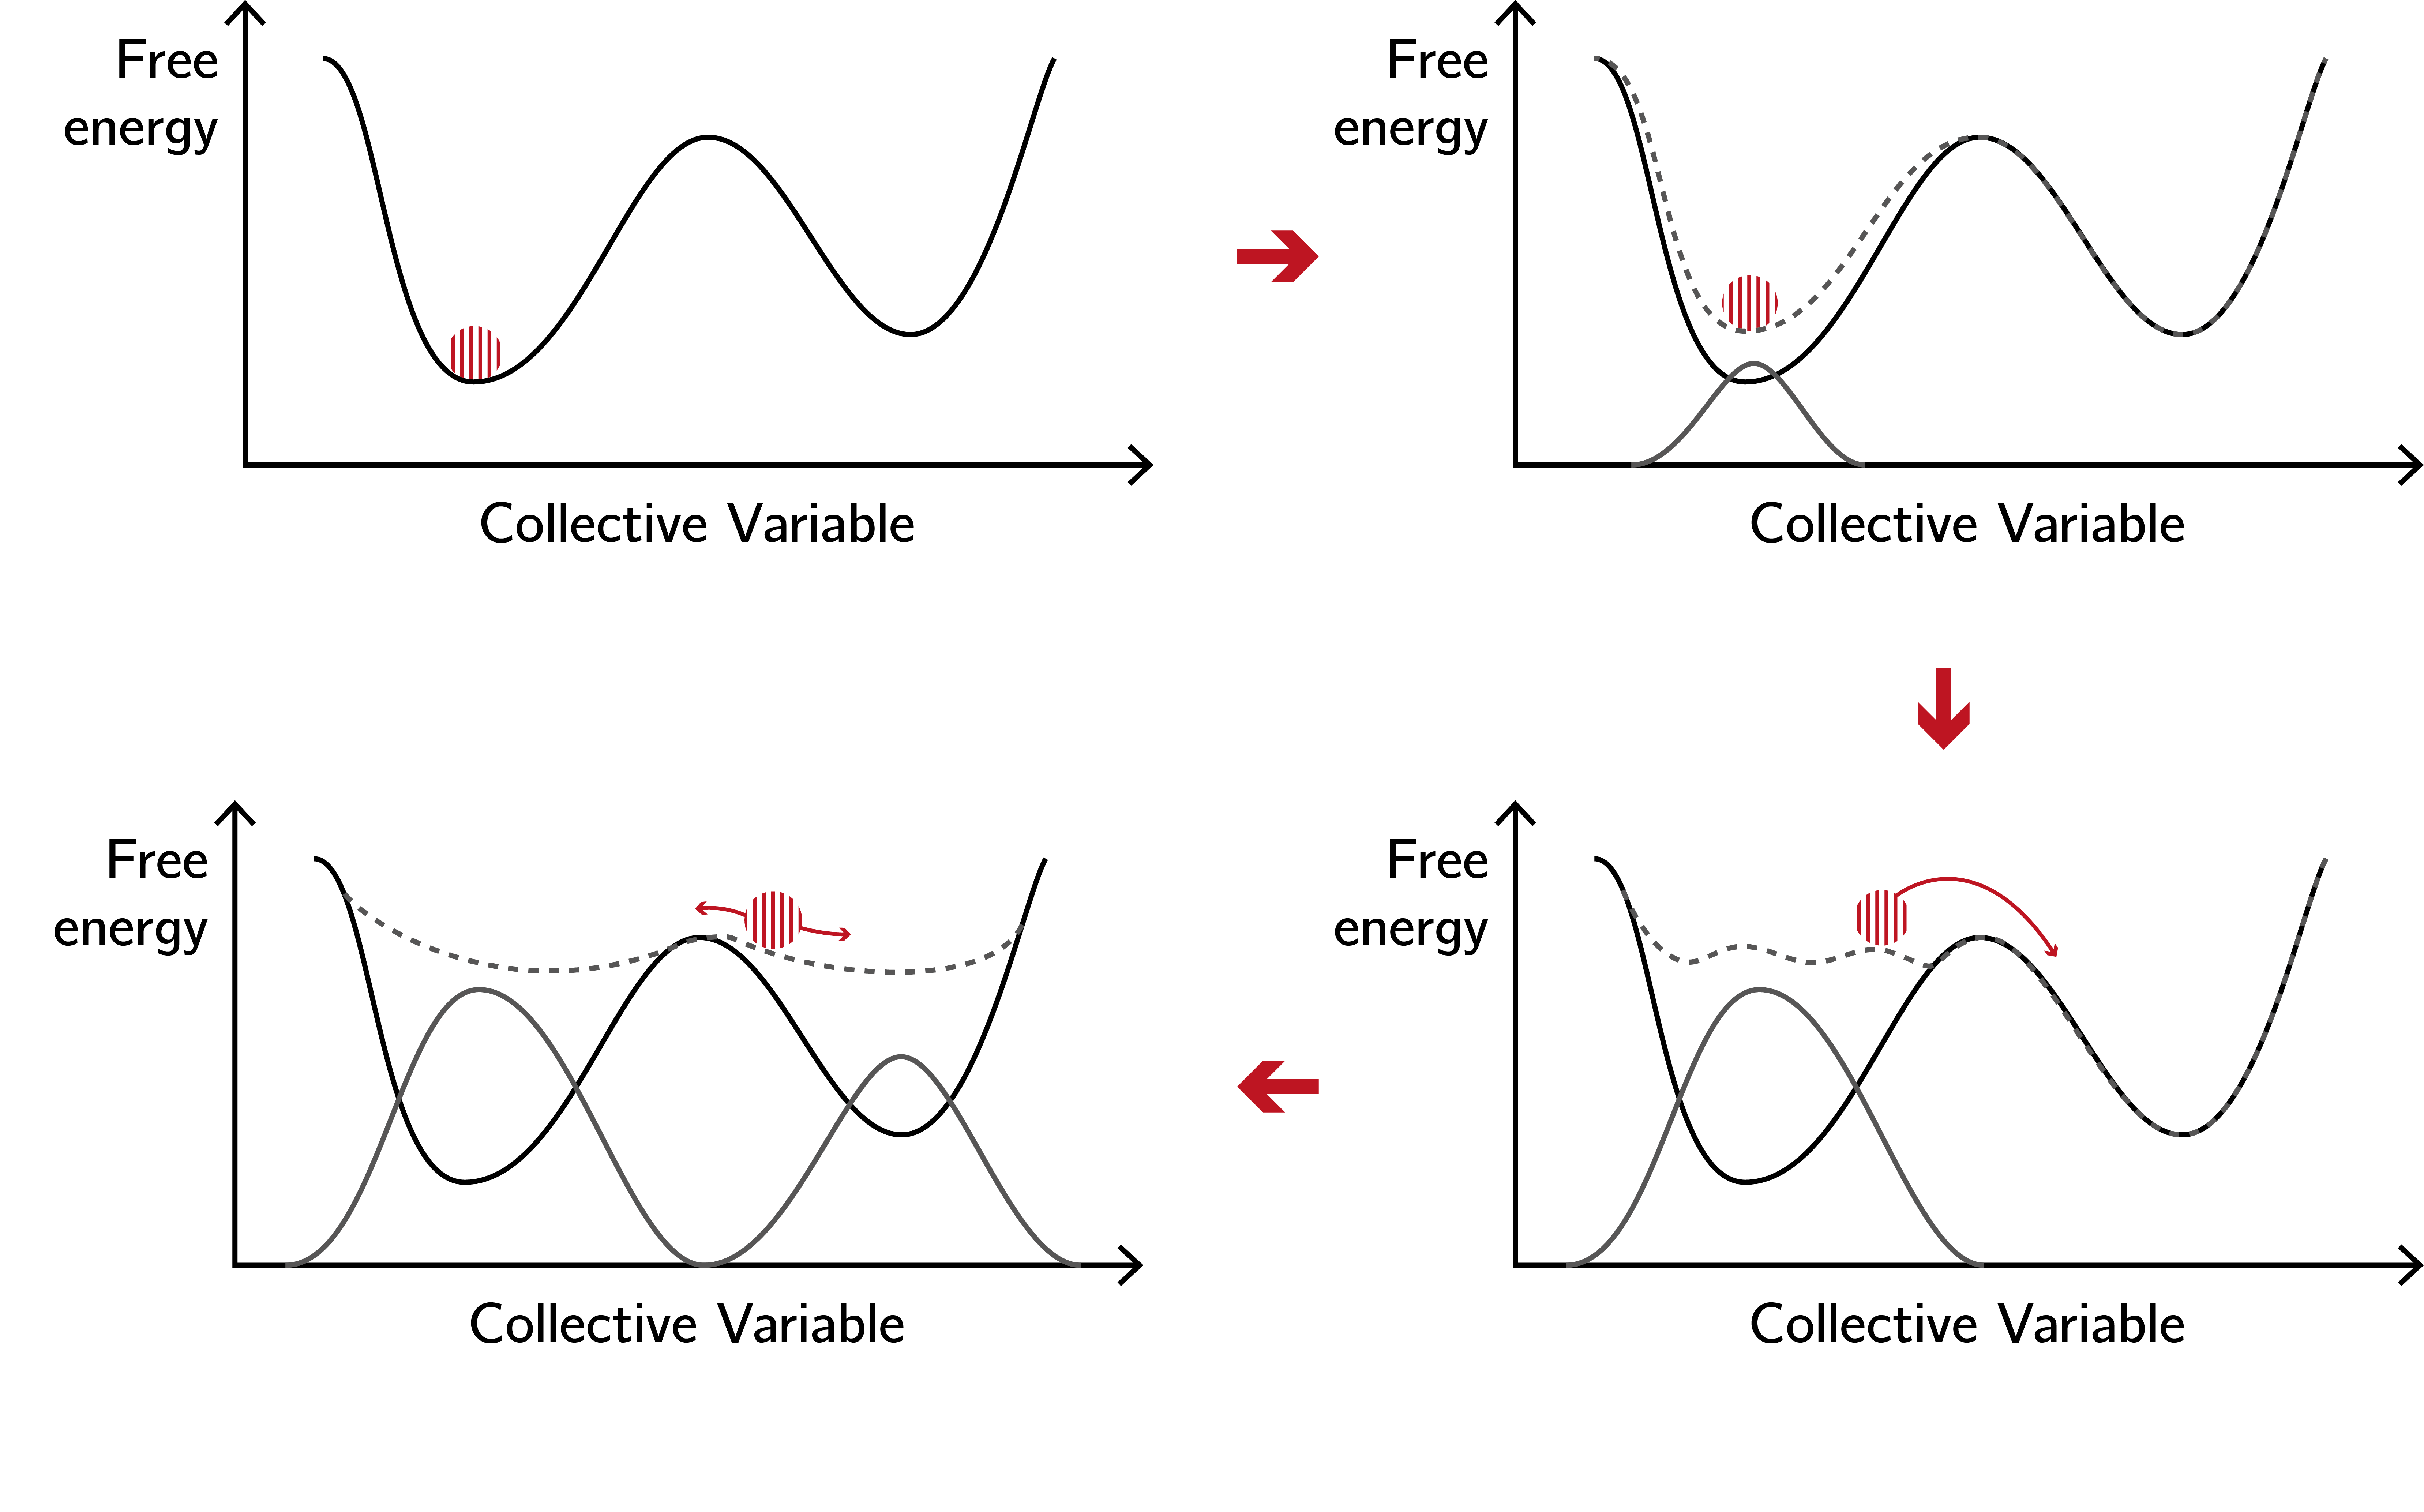
\includegraphics[width=\columnwidth]{./images/MetaD.png}
\caption[Metadynamics algorithm]{Time evolution of a system in a metadynamics simulation. The free 
energy surface of a system, $F(s)$, as a function of 
a collective variable, $s$, is represented as well as the biases (bellow the FES) and the 
CV-space position of the system (black circle). The dashed lines represent the FES that the 
biased system is experiencing due to the bias. The figure was adapted by Adriana Pérez Conesa 
based on the figure of Bussi and Branduardi.\cite{bussi2015free_v2} }
\label{MetaD_Figure}
\end{figure}

Figure \ref{MetaD_Figure} represents schematically the evolution of a system in a metadynamics 
simulation. The free energy surface of a system, $F(s)$, as a function of 
a collective variable, $s$, is represented as well as the bias (bellow the free energy surface) and 
the CV-space position of the system (striped circle). A free energy surface (\gls{fes}) is a 
projection of the free energy of the system onto a few CVs that represent its relevant states. 
The system is initially in the left free energy basin and if the barrier to jump to the right 
basin is much higher than $k_\text{B}T$, the system will only explore the left basin. In 
metadynamics 
a bias potential is added in the form of gaussians in the regions of CV-space where the system 
has been (Figure \ref{MetaD_Figure} top right) elevating the effective free energy surface of 
the system. If the right basin accumulates enough bias, the barrier is small enough for the 
system to jump to the right basin and start exploring it and filling it with bias (Figure 
\ref{MetaD_Figure} bottom right). When the right basin is also filled with bias and effective 
free energy of the system becomes flat enough, the system diffuses in CV-space going from one 
state to the other (Figure \ref{MetaD_Figure} bottom left). From the deposited bias the 
original free energy surface of the system can be calculated.

The basis of WTMetaD is the following time-dependent bias potential:
\begin{equation}\label{bias}
V(s,t)=\sum^{n}_{k=1}W
\exp{\left[-\frac{1}{\gamma-1}\beta V_{k-1}(s_k) \right]}
\eu^{\left(s-s_k\right)^2/\sigma^2}
\end{equation}
This is the bias potential added to the system hamiltonian at time $t$, where 
$n\tau<t<(n+1)\tau$. At this time it consists of $n$ Gaussians deposited which were deposited 
every 
$\tau$ steps. 

Each of the terms in the sum is a deposited gaussian ($\eu^{\left(s-s_k\right)^2/\sigma^2}$) at 
a 
position visited by system, $s_k$, with a spread $\sigma$. The initial height of the Gaussians is 
$W$ but the height decays exponentially in the regions that already have bias deposited due to the 
factor $\exp{\left[-\frac{1}{\gamma-1}\beta V_{k-1}(s_k) \right]}$. The rate of decay is controlled 
by $\gamma$ known as bias factor which is a simulation input parameter. The exponential decay of 
heights is the difference between the initial metadynamics algorithm to WTMetaD.

\begin{figure}
\centering 
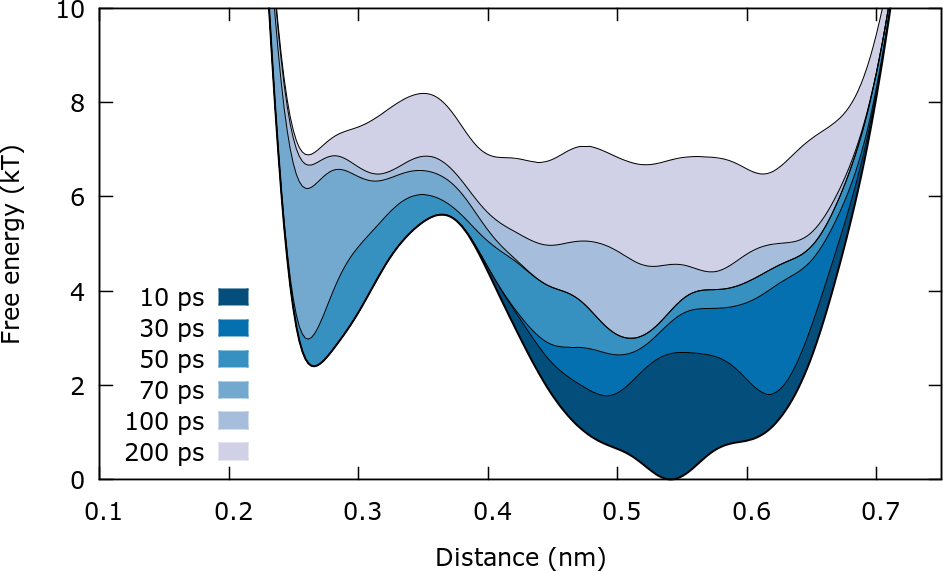
\includegraphics[width=10cm]{./images/FES_PLUMED.png}
\caption[Metadynamics free energy surface]{Free energy surface of a system as a function of 
distance 
(lower curve). Since the 
system is being simulated with metadynamics bias accumulates with time (upper curves) filling the 
free energy minima. Reproduced from the PLUMED2 manual\cite{Tribello2014}. }
\label{FES_PLUMED}
\end{figure}

 Figure \ref{FES_PLUMED} shows the free energy surface 
of a system as a function of one CV, distance,  and how the FES is filled as a function of time. 
Initially the 5$k_\text{B}T$ barrier makes the system oscillate within the right basin. After 
\SI{50}{\pico\second} so many Gaussians have been deposited in 
this region of the CV that the bias has reduced the 5$k_\text{B}T$ barrier to 2$k_\text{B}T$. 
This 
allows the system to have a fluctuation by which it jumps to the left basin. At this point 
the system starts to explore the left basin and fill it with bias. Once the two states have 
been filled with Gaussians the FES becomes somewhat flat which allows the system to cross from 
one state to the other. At this point the time-evolution of the CV becomes diffusive and if 
the heights of the Gaussians deposited are low: the simulation has converged. At convergence 
the FES experienced by the system is the unbiased FES scaled by the bias factor. 

In a converged simulation the free energy of the unbiased system as a function of the 
collective variable, 
$F(s)$, is:
\begin{equation}
F(s)=-\frac{\gamma}{\gamma-1}V(s,t)+c(t)
\end{equation}
Therefore a part from an additive constant, $c(t)$, the FES can be obtained from the simulation
deposited bias. Free energy differences between the states are calculated integrating the 
FES over their basins $A$ and $B$:
\begin{equation}
\Delta F_{A,B}=-k_\text{B}T\log\left(\frac{\int_A\eu^{-\beta F(s)}ds}{\int_B\eu^{-\beta 
F(s)}ds}\right) 
\end{equation}

WTMetaD was proposed in order to fix a problem of the original metadynamics formulation. In 
the prior formulation the height of the Gaussians deposited was constant. After the filling of 
the free energy wells of the system the bias would keep depositing forever so that the 
simulation would explore higher and higher free energy regions of CV space. It was up to the 
user to stop the simulation. WTMetaD has been proven to converge asymptotically\cite{Dama2014} 
therefore giving clear convergence conditions: the gaussian heights should be small and the CVs 
should have diffusive dynamics. 

Access to FES is not exclusive for enhanced sampling simulations. In any ergodic 
MD simulation the FES as a function of a CV, $s$, can be obtained from its 
probability distribution, $P(s)$:
\begin{equation}\label{hist2}
F(s)=-k_\text{B}T\log\left(P(s)\right)+c
\end{equation}
If the system is not ergodic, metadynamics or some other enhanced 
sampling technique must be 
used. In the case of metadynamics, Equation \ref{hist2} cannot be used directly since the 
distribution of the simulation is non-Boltzmann due to the bias. Nevertheless, the unbiased 
distribution can be estimated calculating a weighted histogram with the biased data in which the 
weights compensate biasing. This process is known as \textit{reweighting} and it can 
be done in several ways. The most accurate is the one developed recently by Tiwari and Parrinello 
which estimates the time dependent constant, $c(t)$, and in this way calculates 
exactly the bias at each step of the simulation.\cite{ReweightTiwary2015} This reweighting scheme 
uses the following 
weight for a given data point of value, $s$,  sampled at time $t$:
\begin{equation}
w(s,t)\propto\exp\left[\beta\left(V_\text{MetaD}(s,t)-c(t)+V_\text{ext}(s)\right)\right]
\end{equation}
Where $V_\text{MetaD}(s,t)$ is the WTMetaD bias, $c(t)$ the time-dependent constant and 
$V_\text{ext}(s)$ any 
additional bias added (for example only to study a certain region of the CV). Reweighting is a 
very powerful technique because it allows to project the FES on collective variables different 
than 
the ones biased in the simulation. The typical metadynamics approach is to find suitable CVs 
to converge the simulation and then reweight on to any other CV to explore the chemistry of 
the system. 

We will briefly enumerate the input parameters of a WTMetaD simulations and how they 
should be selected. In general, metadynamics is fairly robust with respect to parameter choice.
\begin{itemize}
 \item \textbf{Bias factor, $\gamma$:} It regulates the decay of the gaussian heights and 
should be chosen to be similar to the barrier size in units of $k_\text{B}T$. In the limit of 
very 
high $\gamma$ the original formulation of metadynamics is recovered. On the other hand, if $\gamma$ 
tends to 1 unbiased MD are obtained.
\item \textbf{Initial gaussian height, $W$:} It should be chosen to be 1-2$k_\text{B}T$. In 
principle 
it can be higher but it can make the equations of motion unstable due to very high biasing 
forces.
\item \textbf{Gaussian deposition frequency, $\tau$:} It should be roughly equal to the 
autocorrelation time of the CV in order for the system to ``equilibrate'' in between 
depositions. This can be estimated from unbiased simulations.
\item \textbf{Gaussian widths, $\sigma_i$:} Ideally they should be as small as possible to describe 
more accurately the underlying FES, but the smaller the width the slower the convergence. Typically 
it is set to a third or a fifth of the standard deviation of the CV in the narrowest basin in an 
unbiased simulation.
\item \textbf{Collective variables, $s_i$:} The success of metadynamics simulations is mostly 
dependent on the choice of collective variables. Ideally, only one should be used but two are 
the standard and three is also possible and necessary in some cases. Of course, the more CVs are 
biased the slower the convergence. The CVs should capture all the slow motions of the system such 
that when the bias converges there is diffusion in CV space. In many cases CV choice is cumbersome. 
Even if one useful CV has been chosen, there may be hidden orthogonal CVs that are not biased and 
prevent convergence. An example of this can be given in the context of ligand binding. Suppose the 
bias CV is only the distance between the pocket and the ligand. If the pocket is closed by the 
position of a side-chain, until there is a fluctuation and the side-chain opens the ligand will not 
bind. This will result in a decay of the gaussian heights which will barely be deposited and there 
will not be diffusion of the CV in time. To solve this, a side-chain CV should also be
biased. 
\end{itemize}

This section has mostly been based on the following 
reviews\cite{bussi2015free_v2,Valsson2016,Barducci2011}.

\bibliographystyle{achemso}
\bibliography{./library,./extrabib}
          % Capítulo 2
\ChapFrame
\chapter[]{A hydrated ion model of \ce{[UO2]^{2+}} in water: Structure, dynamics, and 
spectroscopy from classical molecular dynamics}\label{art1}
\section{
%Pérez-Conesa, S.; Torrico, F.; Martínez, J. M.; Pappalardo, R. R.; Sánchez
%Marcos, E. 
\textit{J. Chem. Phys.} \textbf{2016},\textit{ 145, 224502--224523}
}
\
\newpage
\ 
\newpage
\includepdf[scale=1,pages=-]{./articles/JCP_2016.pdf}
%\section*{Supplementary Material}
\addcontentsline{toc}{subsection}{Supplementary Material}
\newpage
\ 
\newpage
\includepdf[scale=1,pages=-]{./articles/SI_JCP_2016.pdf}
\ChapFrame
\chapter[]{A general study of actinyl hydration by molecular dynamics simulations using ab 
initio force fields}\label{art2}
\section{
%Pérez-Conesa, S.; Torrico, F.; Martínez, J. M.; Pappalardo, R. R.; Mar-
%cos, E. S. 
\textit{J. Chem. Phys.} \textbf{2019}, \textit{150, 104504--104514}
}
\newpage
\ 
\newpage
\includepdf[scale=1,pages=-]{./articles/JCP_2019.pdf}
\addcontentsline{toc}{subsection}{Supporting Information}
\includepdf[scale=1,pages=-]{./articles/SI_JCP_2019.pdf}
\ChapFrame
\chapter[]{Extracting the Americyl Hydration from an Americium Cationic Mixture in Solution: A 
Combined X-ray Absorption Spectroscopy and Molecular Dynamics Study}\label{art3}
\section{
%Pérez-Conesa, S.; Martínez, J. M.; Pappalardo, R. R.; Sánchez Marcos, E.
\textit{Inorg. Chem.} \textbf{2018}, \textit{57, 8089--8097}
}
\newpage
\ 
\newpage
\includepdf[scale=1,pages=-]{./articles/IC_2018.pdf}
\newpage
\ 
\newpage
\addcontentsline{toc}{subsection}{Supplementary Material}
\includepdf[scale=1,pages=-]{./articles/SI_IC_2018.pdf}
\ChapFrame
\chapter[]{Combining EXAFS and Computer Simulations to
Refine the Structural Description of Actinyl in Water
}\label{art3.5}
\section{
Pending on publication 
}
\newpage
\ 
\newpage
\includepdf[scale=1,pages=-]{./articles/actinyl_XAS.pdf}
\addcontentsline{toc}{subsection}{Supplementary Material}\newpage
\ 
\newpage
\includepdf[scale=1,pages=-]{./articles/SI_actinyl_XAS.pdf}
\ChapFrame
\chapter[Hydration and Diffusion Mechanism of Uranyl in Montmorillonite Clay: MD Using an Ab 
Initio Potential]{Hydration and Diffusion Mechanism of Uranyl in 
Montmorillonite Clay: Molecular 
Dynamics Using an Ab Initio Potential}\label{art4}
\section{
%Pérez-Conesa, S.; Martinez, J. M.; Sanchez Marcos, E. 
\textit{J. Phys. Chem. C} \textbf{2017}, \textit{121, 27437--27444}
}
\newpage
\ 
\newpage
\includepdf[scale=1,pages=-]{./articles/JPCC_2017.pdf}
\addcontentsline{toc}{subsection}{Supporting Information}
\includepdf[scale=1,pages=-]{./articles/SI_JPCC_2017.pdf}
\section[\textit{Erratum}]{\textit{Erratum}}
\begin{figure}
\centering 
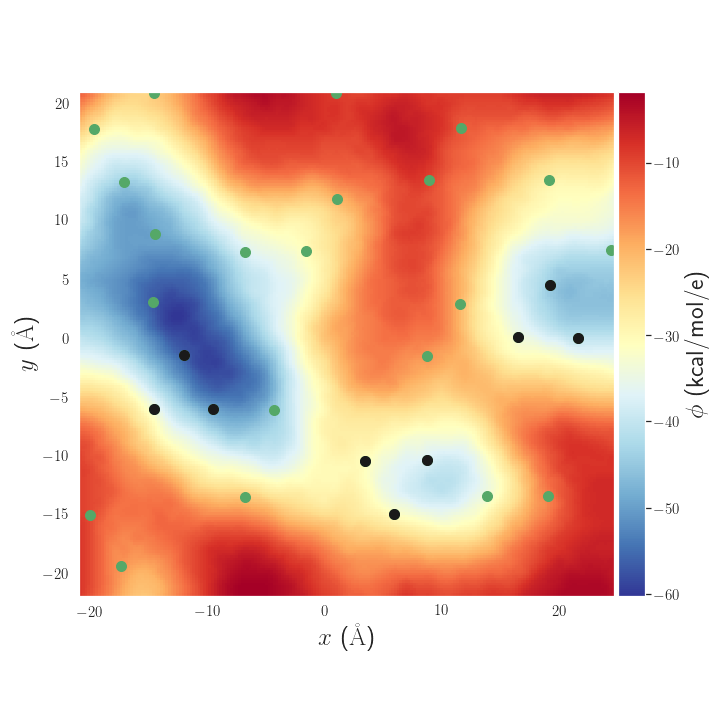
\includegraphics[width=0.75\columnwidth]{./images/erratum_EPS.png}
\caption[Correction to Electrostatic Potential Surface]{Corrected electrostatic potential 
($\phi$) surface at $z=$\SI{-10}{\angstrom} in \si{\kilo\cal\per\mol\per\e} as it should have 
appeared in the article. The published figure had the sign of both axis changed. Mg are 
represented as green circles or black circles if they are part of a site.}
\label{erratum_EPS}
\end{figure}
When preparing the material for the thesis manuscript, I realized that the electrostatic 
potential energy surface published in the article 
of this chapter (Figure 7) was wrong. The correct figure would have had changed signs 
of both the $x$ and $y$ axis. Figure \ref{erratum_EPS} contains the correct information. 

We find that the electrostatic potential is minimum in the regions close to the sites. On the 
contrary to our speculation in the article, the strong interaction with the sites is 
electrostatic. The strength of the interaction is very high which explains the 
low diffusion of the cations. Additionally, the strength of the interaction varies in each 
site due to the different substitution pattern around them. The electrostatic 
potential is screened by the water molecules and the rest of the cations. The strength of this 
screening is different if there is one HI per interlayer or four. The different screening in 
either system explains the difference in cation diffusivity. 

In the section ``Uranyl Diffusion Modeling'', the translational self-diffusion coefficient 
published was mistranscribed. The 
actual value is $D^\text{MD}=0.004\pm0.002\cdot 10^{-5}\si{\centi\meter\squared\per\second}$. 
Fortunately, the parameter that was analyzed, the constrictivity factor was correct.
\ChapFrame
\chapter[]{A local fingerprint for hydrophobicity and hydrophilicity: from methane to 
peptides}\label{art5}
\section{
%Pérez-Conesa, S.; Piaggi, P. M.; Parrinello, M. 
\textit{J. Chem. Phys.} \textbf{2019}, \textit{150,204103--204108}
}\label{art5_sec1}
\newpage
\ 
\newpage
\includepdf[scale=1,pages=-]{./articles/JCP_19_Parrinello.pdf}
\addcontentsline{toc}{subsection}{Supporting Information}
\includepdf[scale=1,pages=-]{./articles/SI_JCP_19_Parrinello.pdf}

\section[Hydrophobicity fingerprint of actinyls]{Hydrophobicity hydrophilicity 
fingerprint of actinyls.}

\begin{table}
\center
\caption[Fingerprint values for actinyls]{Hydrophobicity/hydrophilicity fingerprint values of 
actinyl atoms obtained from the 
simulations of Chapter \ref{art2}.}\label{tableAn}
\begin{tabular}{lccc}
\toprule
&$h$&$h^\text{HI}$&$h^{\text{HI}}_{\text{0-\SI{90}{\degree}}}$\\
\midrule
An       &-7.9   &  -5.2 & -  \\
\oyl  & -1.9 &   0.4 & -2.1 \\
\ofs  &0.8&   1.5  &0.5\\
\ce{H2O}    & 1.0&  1.0 & - \\
\ce{CH4}    &-1.0& -1.0 & -  \\
\bottomrule
\end{tabular}
\end{table}

Given the amphiphilic nature of the solvation of actinyls, the simulations carried out in 
Chapters \ref{art1} and \ref{art2} are perfect candidates to study the fingerprint behavior in 
complex cationic systems. We present the fingerprints of the heavy atoms of uranyl as  
representative of the rest of actinyls since due to their similarity in solvation the fingerprint 
values must be very similar even for \ce{[NpO2]^+}. The 
reference values of $S_s$ were calculated from a pure TIP4P-water simulation and a methane 
TIP4P-water simulation. Three versions of the fingerprint were examined:
\begin{itemize}
 \item $h$: uses the RDF between the atom of interest 
and all water molecules.
\item $h^\text{HI}$: uses the RDF between the fingerprinted atom and all bulk water molecules 
excluding 
the first-shell.
  \item $h^\text{HI}_\text{0-\SI{90}{\degree}}$: uses the 0-\SI{90}{\degree} angle-solved RDF 
between 
the fingerprinted atom and all bulk water molecules. The 0-\SI{90}{\degree} cone is calculated 
in the same fashion as in the angle-resolved RDFs of the \oyl atom in Chapter \ref{art1}.
\end{itemize}

The last two definitions connect with the HIM philosophy by considering first-shell water 
molecules part of the solute and not of the solvent. The fingerprint values are 
collected in Table 
\ref{tableAn}.

The first shell water molecules (\ofs) are correctly labeled as hydrophilic by the fingerprint in 
all 
versions. In contrast, the \oyl atoms are labeled as hydrophilic by $h^\text{HI}$ and 
hydrophobic by $h$. $h^\text{HI}$ is conceptually a better fingerprint since first-shell water 
molecules do not solvate the \oyl atom. Unfortunately, it also misclassifies the \oyl 
atom as hydrophilic.

As we have seen in Chapter \ref{art1}, the solvation of the uranyl atoms is 
very 
anisotropic and standard RDF  can lead to wrong conclusions 
i. e. the \oyl RDF 
includes solvent 
molecules that are in the bridge solvation region and are not solvating the \oyl atom. For 
this reason we decided to use as the fingerprint 
input the 0-\SI{90}{\degree} angle-solved RDF. In this way, the solvent molecules included in the 
RDF are the ones that solvate the atom. $h^\text{HI}_\text{0-\SI{90}{\degree}}$ classifies 
correctly 
the \oyl and \ofs atoms but it considers \ofs to be less hydrophilic than 
bulk water molecules.

The fingerprint classifies the actinoid cation as hydrophobic which is clear\-ly an artifact. 
In 
Section \ref{art5_sec1} this effect was also described for \ce{Na^+}. The order imposed on the 
solvent structure by the 
doubly charged cation is very high and thus obtaining $h$ values much lower than methane. 

In conclusion, the fingerprint appears to be unfit to classify the central atoms of cations 
with charge higher or equal to one. For the rest of the heavy atoms of the hydrated ion mixed 
results are obtained.

The fingerprint is too coarse for complex solutes like actinyls. A future improved 
fingerprint could probably make use of orientational pair entropy in addition to some technique to 
consider the anisotropicity of the solute in complex environments. 

%%%%%%%%%%%%%%%%%%%%%%%%%%%%%%%%%%%% apéndices %%%%%%%%%%%%%%%%%%%%%%%%%%%%%%%%%%%%%%%%%
\ChapFrame
\chapter[Results and Discussion]{Results and Discussion}
In this section we will review the main results of the thesis. Their significance and relation to 
other works in the literature will be discussed.

\section[Force Fields Development]{Force Field Development}\label{ffdevelopment}
\subsection[Actinyl Force Fields In Solution]{Actinyl Force Fields In Solution}
The largest body of force fields designed concerned the actinyl cations. In particular 
\ce{[AnO2*(H2O)5]^{2+}} for An=U, Np, Pu, Am and \ce{[NpO2*(H2O)5]^{+}}. This work was 
rooted in a chapter of the thesis of F. Torrico, a former PhD student of the group\cite{thesisFran}.

These are the first hydrated ion models for actinyls and 
the first to have a molecular cation rather than a monoatomic cation. Using an interaction 
potential which contains the \textit{ab initio} information of the system is very convenient in 
actinoid systems. Unlike other compounds, the lack of experimental data complicates parametrizing
actinoid compounds empirically\cite{Ions_in_sol_and_Marcus_2016}. 

\begin{figure}
\centering 
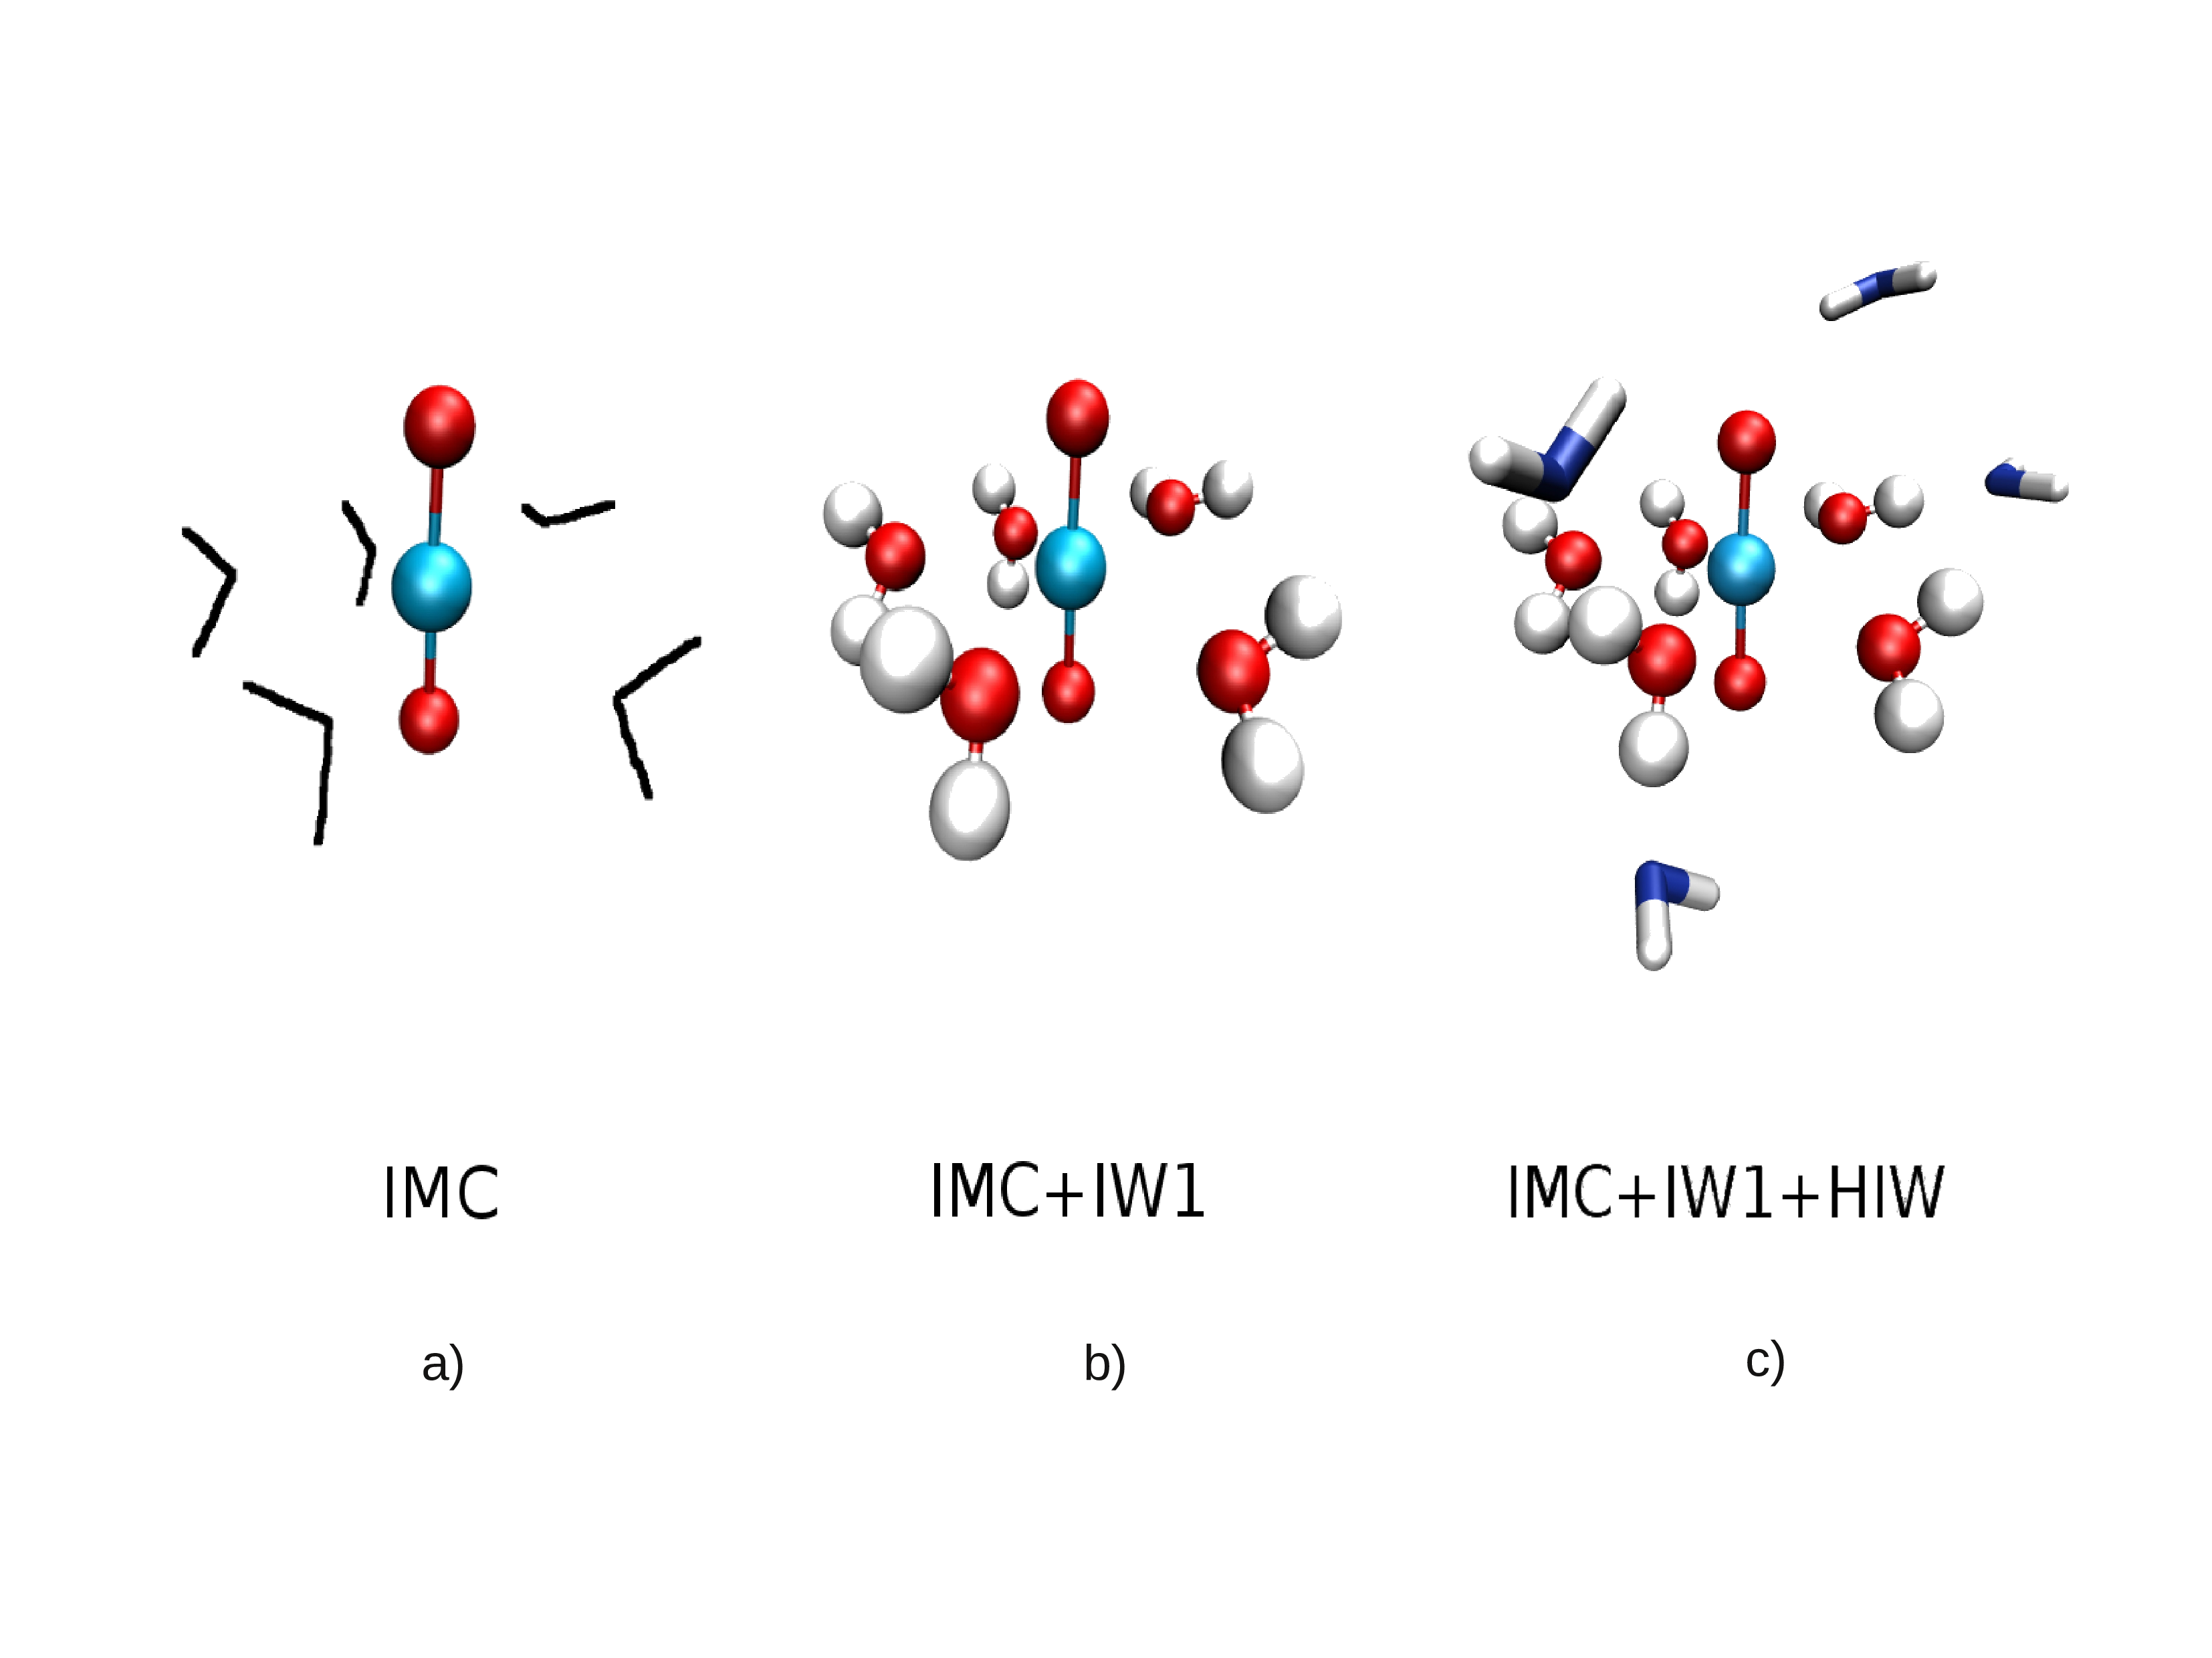
\includegraphics[width=10cm]{./images/IMCIW1HIW.png}
\caption[Components of the Hydrated Ion Model]{Schematic representation of the components of 
the HIM force field of actinyl ions. The 
ball and stick representation shows the atoms involved in each of the terms. In a) the first shell 
is not fully 
drawn since it does not participate in the IMC but they are added to calculate the interaction 
energies for the IMC following the HIM. }\label{HIM_actinyl}
\end{figure}

The actinyl force fields were developed using as reference structure the pentahydrate 
cation, 
\ce{[AnO2*(H2O)5]^{2+/+}}. The interaction potential was split into four components:
\begin{equation}
E=E_\text{IMC}+E_\text{IW1}+E_\text{HIW}+E_\text{W-W}
\end{equation}
The first three components are shown in Figure \ref{HIM_actinyl}. The 
first interaction 
potential is the Intra-Molecular Cation (\gls{imc}). This interaction potential controls the motion 
within the molecular cation, \ce{[AnO2]^{2+/+}}. It has the following mathematical expression:
\begin{equation}\label{eq1}
E_{\text{IMC}} = \sum_{i}^{ \substack{\text{O}_{\text{yl}} \vspace{0.02cm}\\ \text{sites} } }\left(
\frac{C_{4}^{\text{AnO}_{\text{yl}   }} }  {r_{\text{AnO}_{\text{yl,i}}}^{4} }  +
\frac{C_{6}^{\text{AnO}_{\text{yl}   }} }  {r_{\text{AnO}_{\text{yl,i}}}^{6} }  +
\frac{C_{8}^{\text{AnO}_{\text{yl}   }} }  {r_{\text{AnO}_{\text{yl,i}}}^{8} }  \right. \left.+
\frac{C_{12}^{\text{AnO}_{\text{yl}   }} }  {r_{\text{AnO}_{\text{yl,i}}}^{12} }\right)  +
\sum_{i}^{\substack{\text{O}_{\text{yl}} \vspace{0.02cm}\\ 
\text{sites} }}
\frac {q_{\text{An}} q_{\text{O}_{\text{yl,i}}}} { r_{\text{AnO}_{\text{yl,i}}} }
\end{equation}
The second term (Equation \ref{eq2}) is the ion-first shell water interaction (\gls{iw1}). In our model 
we have assumed that the first-shell
water molecules to be rigid and have the geometry of the gas phase optimization of the 
hydrated 
ion. 
The IW1 term makes the aqua ion flexible. It has the following mathematical expression:
\begin{equation}\label{eq2}
E_{\text{IW1}} = \sum_{i}^{ \substack{\text{AnO}_{\text 2} \vspace{0.02cm}\\ \text{sites} }}
  \frac {C_{4}^{\text{iO}_{\text I}}}{r_{\text{iO}_{\text I}}^{4}}
+ \frac {C_{6}^{\text{iO}_{\text I}}}{r_{\text{iO}_{\text I}}^{6}}
+ \frac {C_{8}^{\text{iO}_{\text I}}}{r_{\text{iO}_{\text I}}^{8}} 
+ \frac {C_{12}^{\text{iO}_{\text I}}}{r_{\text{iO}_{\text I}}^{12}} 
+ \sum_{i}^{ \substack{\text{AnO}_{\text 2} \vspace{0.02cm}\\ \text{sites} }}\,
\sum_{j}^{ \substack{\text{1}^{\text {st}}\text{ shell water}\vspace{0.02cm}\\ \text{sites} }}
\frac{q_{\text{i}}q_{\text{j}}}{r_{\text{ij}}}\\
\end{equation}
The final term (Equation \ref{eq3}) is the hydrated ion-bulk water interaction potential (\gls{hiw}). 
This term parametrizes 
the
interaction of the hydrated ion with any of the bulk water molecules (second shell and further). It 
has the 
following mathematical expression:
\begin{equation}\label{eq3}
E_{\text{HIW}} = \sum_{i}^{\substack{\text{HI} \vspace{0.02cm}\\ \text{sites} }} 
\sum_{j}^{\substack{\text{water} \vspace{0.02cm}\\ \text{sites} } }\left(
\frac{C_{4}^{ij}}{r_{ij}^{4}}+\frac{C_{6}^{ij}}{r_{ij}^{6}}+\frac{C_{8}^{ij}}{r_{ij}^{8}}\right.+
\frac{C_{12}^{ij}}{r_{ij}^{12}} +
\left.\frac{q_{i}q_{j}}{r_{ij}}\right)
\end{equation}
The employed bulk water model was TIP4P\cite{TIP4P_JChemPhys_Jorgensen_1983}. 

The partial charges appearing in Equations \ref{eq1}-\ref{eq3} were assigned with the 
Merzt-Kollmann 
method\cite{MK1_Kollman_JCompChem_1984,MK2_MerzKollman_JCompChem_1990}. These charges were 
calculated in the gas pha\-se QM minimum energy structures and using a wavefunction 
polarized by bulk solvent represented by a Polarizable Continuum Model (\gls{pcm} 
)\cite{PCM1_ChemPhys_Tomasi_1981,PCM2_JChemPhys_Tomasi_1997}. In 
the case 
of \ce{[NpO2*(H2O)5]^{+}} only the actinyl unit was given partial charges. Due to the low charge 
transfer and polarization of this monocation, the first-shell geometries and charges were taken to 
be 
equal to those of the TIP4P water model. The coefficients of the 
force fields were parametrized with a series of QM scans. $E_\text{IMC}$ and 
$E_\text{IW1}$ were parametrized with deformations following the main normal modes of the 
pentahydrate: symmetric and asymmetric An-\ce{O_{yl}} tension, \ce{O_{yl}}-An-\ce{O_{yl}} bending 
and lengthening of a An-\ce{O_{W1}} distance. $E_\text{HIW}$ was parametrized with scans of a 
second-shell water molecule moving around the hydrated ion at different distances and orientations. 
The root mean square errors of the fits were about 1-\SI{3}{\kcalmol}. All the interaction 
potentials 
were 
calculated specifically for every cation except for the HIW potential which was proven to be very 
similar across the cations studied. The level of theory for the quantum chemistry calculations was 
B3LYP with Stuttgard semi-relativistic pseudopotentials and their recommended basis sets on 
actinoids and aug-PVDZ on light 
atoms\cite{B3LYP1,B3LYP2_GAUSSIAN,DunningBasisSet3_Dunning_JChemPhys_1993,RECPStuttgart}. In all 
electronic structure calculations the first shell of water molecules was included. This was done 
so that even the IMC truly models the molecular cation in the aqueous medium. 

It is important to use a high level of theory in order to shed light on the complicated 
XAS spectroscopy of actinyls. For this reason a NEVPT2\cite{NEVPT2_1,NEVPT2_2,NEVPT2_3}-level force 
field was developed for  \ce{[NpO2*(H2O)5]^{+}}. In this way we treated explicitly the 
multi-reference nature of the cation instead of using the mean field 
strategy of DFT. The active 
space chosen for the CASSCF consisted of the atomic-like $f$-orbitals of the actinoid and four 
$\pi/\pi^*$ and two $\sigma/\sigma^*$ molecular orbitals formed by \ce{O_{yl}} $p$-orbitals and 
actinoid bond-participating $f$-orbitals. This resulted in a CASSCF(n,10) space where n is six plus 
the number of actinoid unpaired electrons. A state average 
between the doubly degenerate\newline ground state solutions was performed. All calculations were 
run 
using the RI 
and RIJK approximations.\cite{RI1_Dunlap_JChemPhys_1979,RI2_JCompChem_Alsenoy_1988,
RI3_Kendall_TheoChemAcc_1997,
RI4_Ahlrich_ChemPhysLett_1995,RI5_Ahlrich_TheoChemAcc_1997} to reduce the scaling with basis set 
size. The chosen basis sets were ma-def2-TZVP for O, def2-SVP for H, and 
\newline SD(60,MWB)//DEF-TZVP for 
actinoids\cite{Def2weigend2005,ma-Def-rappoport2010,RECPStuttgart}.


Going from the DFT level of theory to the NEVPT2 level of theory does not change significantly any 
of the properties of the actinyls in solution. The only exception is bondlengths which are 
increased a few hundredths of an angstrom for the An-\ce{O_{yl}} distances and decreased a few 
hundredths of an \newline angstrom for the An-\ce{O_{W1}} distances. The sensitivity of EXAFS 
spectrum is so 
high that such small changes in structure generate significant changes in the spectrum. This 
explains 
the interest in the use a very high level of theory potential energy surface. 

Although these systems have been studied in the literature with \textit{ab initio} 
MD\cite{JACS_Buhl_2005} or with
QM/MM\cite{JPhysChemA_Frick_2009}, they were highly limited by the simulation times, system 
size and quantum mechanical level. 
This last aspect is particularly important given the size of the second-shell. 
\textit{Ab initio} force fields provide a cost-effective solution to have near-QM 
forces spending classical MD CPU hours. Of course, the price to be paid is in human hours of force 
field development. 

Despite there are many force fields for 
uranyl\cite{JMolStr_Wipff_1996,JPhysChem_Wipff_1993,JPhysChemA_Kerisit_2013,JACS_Roos_2005,
PhysChemChemPhys_Pomogaev_2013,Duvail2019}, the first actinyl force field beyond uranyl was 
developed by 
Maggin's group\cite{PhysChemChemPhys_Pomogaev_2013,PhysChemChemPhys_Tiwari_2014}. 
They realized the importance of many body effects such as polarization of the first shell and their 
QM calculations were done including four water molecules in the first-shell. We went one step 
further and implemented the full HIM philosophy to the force field: differentiation of first-shell 
and bulk water molecules, by partial charge transfer and full hydration shell in the QM 
calculations. 
Our force fields are the first force fields to explicitly parametrize bulk water-HI interactions 
through the HIW potential, making them particularly suitable to describe the second shell region. 
In addition, other force fields observe residence 
times of the first shell shorter than 
experiment\cite{PhysChemChemPhys_Tiwari_2014,ChemRev_Helm_2005,chem_aq_ions_Richens,thesisAPanasci}
. We observe none, which is what is expected given the simulation time. 

The complexity of our potential development and the number of parameters fitted makes our set of 
force fields highly versatile to derive actinyls under different environments due to their 
first-principles nature. Moreover, we were able to increase even 
further the accuracy to develop a NEVPT2-level force field for the neptunyl monocation . A 
proof of its high 
accuracy is its ability to reasonably reproduce experimental data of a wide variety of types: 
structure, dynamics, spectroscopy and thermodynamics. 

Unfortunately, the interaction potential functional form prevents the use of combination rules. 
Therefore, they are essentially limited to the hydrated ion in pure water. This is the ``one 
system, one force field'' problem of the HIM. Fortunately, in the case of actinyls the 
transferability of the HIW potential, the potential requiring the most QM calculations, avoids 
having to parametrize it for each actinyl. In this way, only the IW1 and IMC potential must be 
parametrized for each particular actinyl.

\subsection[Auxiliary \ce{Am^{3+}} force field]{Auxiliary \ce{Am^{3+}} force field}

The force field of \ce{[Am*(H2O)8]^{3+}} was generated as an auxiliary tool for a greater goal. It 
was 
developed \textit{ad hoc} to reproduce the experimental EXAFS spectrum of \ce{Am^{3+}}. This 
was done in order to have a better insight in the experimental EXAFS 
spectrum of an  \ce{Am^{3+}}/\ce{AmO2^{2+}} mixture since only the EXAFS of a pure
\ce{Am^{3+}} aqueous solution has been recorded. The QM level of theory used was MP2 using a 
Stuttgart
semirelativistic 
pseudopotential\cite{Dolg_RECP} with the recommended basis set on Am and 
cc-PVTZ\cite{DunningBasisSet1_Dunning_JChemPhys_1989,DunningBasisSet4_Dunning_JChemPhys_1992,
DunningBasisSet3_Dunning_JChemPhys_1993,DunningBasisSet2_Dunning_JChemPhys_1994} on light atoms. The 
pseudopotential used includes in the core the f-orbitals since they are internal (unlike in 
actinyls) and do not participate in bonding. In this way the complex can be modeled using 
closed-shell techniques. The structure was minimized using $S_{8}$ symmetry. 
RESP\cite{RESP_JPhysChem_Kollman_1993} partial charges were used for the interaction potential. 
These charges were calculated in the minimized geometry using a wavefunction calculated with the 
PCM method\cite{PCM1_ChemPhys_Tomasi_1981,PCM2_JChemPhys_Tomasi_1997}. Harmonic bond and harmonic 
angular terms were added to keep the structure of the hydrate with equilibrium bondlenths and 
angles taken from the optimized structure. The force constants were fitted to reproduce the 
experimental EXAFS spectrum of \ce{Am^{3+}} using the structures generated by the MD simulation. 
Lennard-Jones 
parameters of TIP4P were added to the first-shell water molecules to interact with the TIP4P bulk 
water molecules.

\subsection[Hydrated Ion-Clay Interaction Potential]{Hydrated Ion-Clay Interaction Potential}
\begin{figure}
\centering 
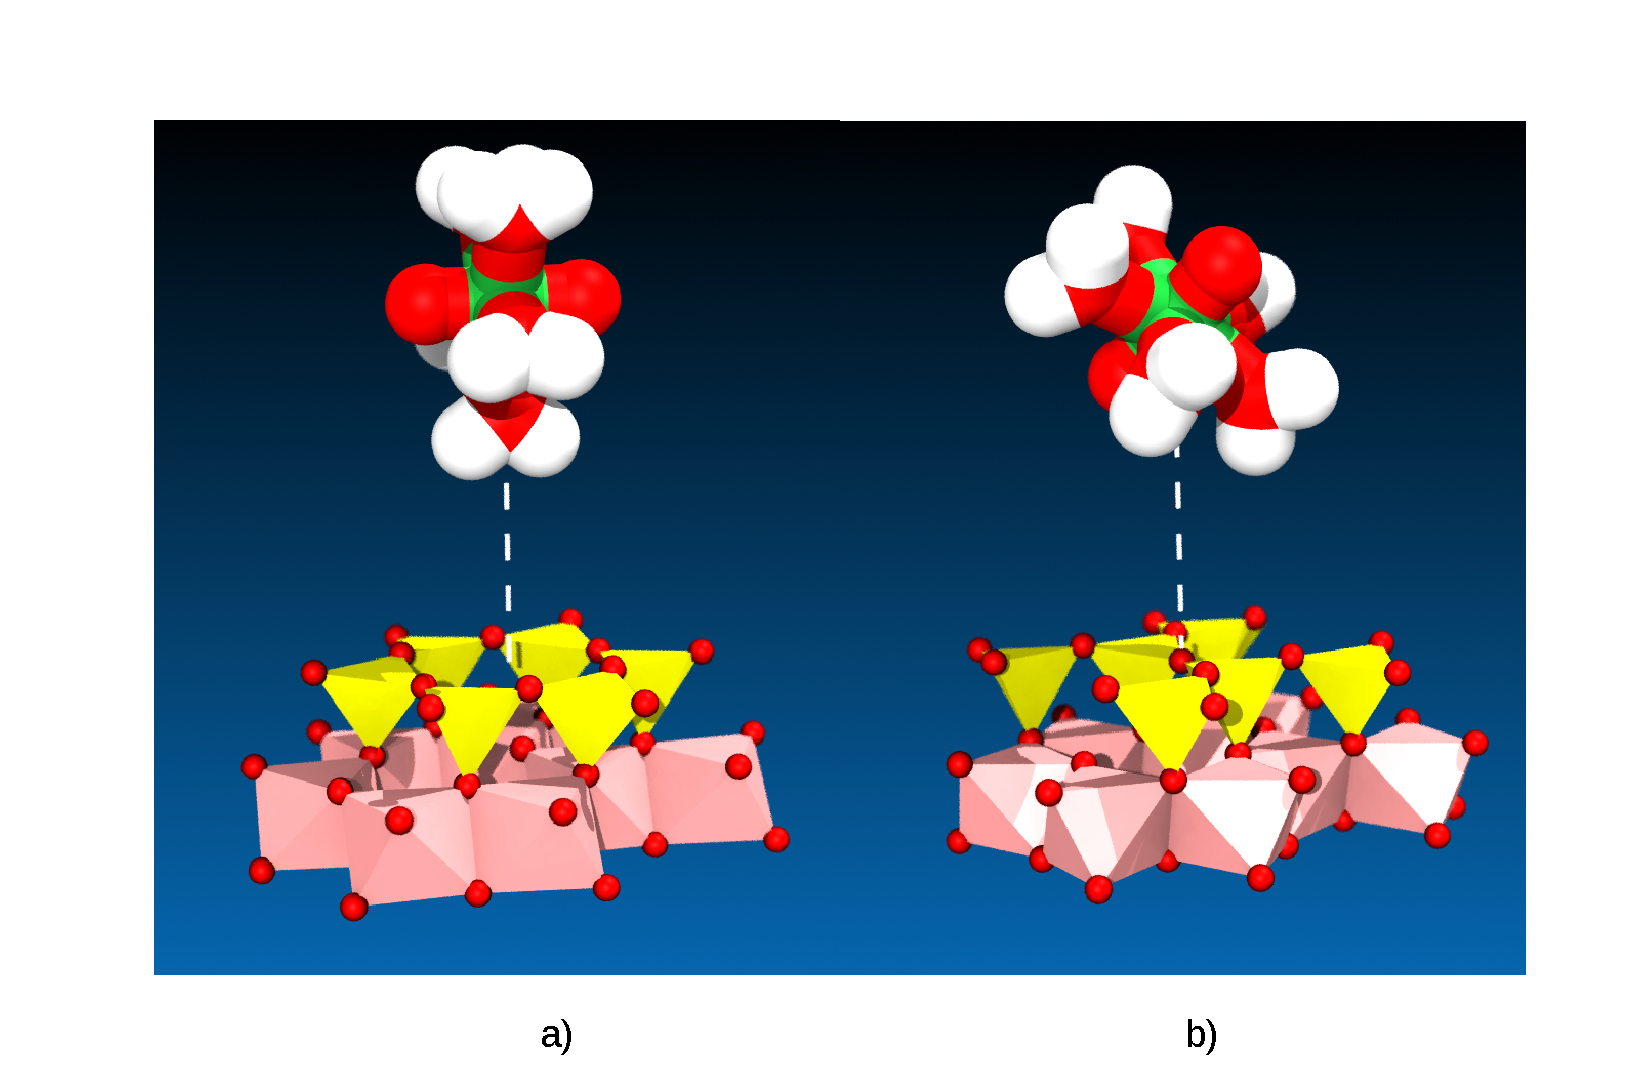
\includegraphics[width=10cm]{./images/scan.pdf}
\caption[QM scans used to parametrize the HIC]{Some of the clay cluster-hydrated ion scans 
used to parametrize the HIC 
potential. a) Hexagonal center scan with a uranyl axis tilt angle of 90º with respect to the 
surface normal. b) O-center cluster with a tilt angle of 45º. The color coding is as follows: Al 
octahedra (pink), Si tetrahedra (yellow), O atoms (red), uranium atoms (green), and H atoms (white)  
}
\label{scan}
\end{figure}

For the simulations of uranyl in montmorillonite clay interlayers the HI clay interaction (\gls{hic}) 
did not exist in the literature. A new strategy had to be developed since this was the first time 
the interaction of a HI with a surface was being studied. In the 
literature\cite{PhysChemChemPhys_Greathouse_2005,EnviSciTech_Greathouse_2006,JHazMat_Yang_2013,
JHazMat_Liu_2013,MolSim_Cygan_2014,
InorChemFronteirs_Zhang_2015,ClayMinSoc_Zaidan_2003,ClayMinSoc_Greathouse_2005} the 
Wipff-Guilbaud model of uranyl with combination rules was used, and therefore, to the best of 
our 
knowledge, this force field is the 
first \textit{ab initio} force field for actinyl-clay systems.


The force field was parametrized from 
the interaction energies of QM scans of \ce{[UO2*(H2O)5]^{2+}} approaching a
cluster of atoms carved from the clay surface (Figure \ref{scan}). The level of theory for the QM 
calculations was MP2 with 
RI\cite{RI1_Dunlap_JChemPhys_1979,RI2_JCompChem_Alsenoy_1988,RI3_Kendall_TheoChemAcc_1997,
RI4_Ahlrich_ChemPhysLett_1995,RI5_Ahlrich_TheoChemAcc_1997} and 
RIJCOSX\cite{RIJCOSX_ChemPhys_Nesse_2009} scaling reduction techniques due to the large size of the 
systems. U, Al and Si were described by Stuttgart semirelativistic pseudopotentials and their 
recommended 
basis sets\cite{U_ecpbasis,H-Rn_ECPbasis_PhysChemChemPhys_Ahlrichs_2005}; O and H were described by 
the 
aug-cc-PVDZ basis 
sets\cite{DunningBasisSet1_Dunning_JChemPhys_1989,DunningBasisSet2_Dunning_JChemPhys_1994,
DunningBasisSet3_Dunning_JChemPhys_1993,
DunningBasisSet4_Dunning_JChemPhys_1992,DunningBasisSet5_Dunning_JChemPhys_1996}. The interaction 
potential function had the following mathematical definition: 
 \begin{align} \label{eq_EHIC}
 E_\text{HIC}=& E_{\text{Coul.}}+E_{\text{non-Coul.}} \\ \nonumber
=&\sum_{i}^{\text{aqua ion}}\sum_{j}^{\text{clay}}\,\frac{q_iq_j}{r_{ij}}
+\sum_{i}^{\ce{U},\,\ce{O_{yl}},\,\ce{O_{I}}}\,\sum_{j}^{\ce{O_{clay}}}\,\frac{C_4^{ij}}{r^4_{ij}
} +
 \frac{C_6^{ij}}{r^6_{ij}}+\frac{C_8^{ij}}{r^8_{ij}}+\frac{C_{12}^{ij}}{r^{12}_{ij}} \nonumber
 \\&+\sum_{i}^{\ce{O_{yl}}}\,\sum_{j}^{\ce{Si}}\,\frac{C_4^{ij}}{r^4_{ij}}+
 \frac{C_6^{ij}}{r^6_{ij}}+\frac{C_8^{ij}}{r^8_{ij}}+\frac{C_{12}^{ij}}{r^{12}_{ij}} \nonumber
\end{align}
The root mean square error of the fit was $\sim$\SI{5}{\kcalmol}, a reasonable value
considering that the interaction energies can be as low as \SI{-100}{\kcalmol}. Structures 
obtained from the MD trajectories were used as a test set of data to check if the 
HIC potential reproduced the quantum interaction energies in structures outside of the 
training data set. 

 A good indicator of the quality of the force field is that it reproduces the experimental finding 
that the first-shell is identical in the clay as in aqueous 
solution.\cite{GeoCosmoAct_Catalano_2005} This outersphere complex 
formation was not imposed on the model. Therefore it was observed because the force field 
made this 
phenomenon to be favored over a partial dehydration into the tetrahydrate. In addition, the 
tilt-angle of the uranyl axis was compatible with the experimental evidence that showed it to be 
neither perpendicular nor parallel to the clay surface.\cite{MinWatIntClEq_Denecke_1999}

\section[Physico-chemical properties of actinyls in solution]{Physico-chemical properties of 
actinyls in solution}
MD simulations were run on the actinyl hydrated ions in aqueous solution with the 
newly developed HIM \textit{ab initio} force fields. In general, the properties calculated related 
closely to their experimental values. In addition the properties are of a 
wide variety: structure, dynamics, spectroscopy and thermodynamics. This good correlation
with experiment and the fact that the force field is \textit{ab initio} gives us  
confidence when computing properties that cannot be compared to experiment. 

The theoretical 
$\Delta H_\text{hyd}$ of the doubly-charged actinyls was fairly close to the value given by 
Marcus\cite{JChemSoc_Marcus_1986} for uranyl although further away from the value of 
Gibson\cite{JPhysChemA_Gibson_2005}. In the case of  \ce{[NpO2]^{+}}, the $\Delta 
H_\text{hyd}$ value matched the experimental value of 
Gibson\cite{JPhysChemA_Gibson_2005}. 
The translational self-diffusion coefficients of actinyls overestimated their experimental values. 
We found this to be caused by the overestimated diffusivity of water by the TIP4P bulk water 
model since the normalization of the coefficients by those of water 
gave a close agreement between theory and experiment. 

Our estimation of normal mode frequencies 
with respect to infrared and Raman spectra was satisfactory (maximum relative error of 15\%) 
considering 
that the B3LYP potential energy surface limits the model accuracy. If the NEVPT2 force field 
developed for \ce{[NpO2]^{+}} is used in simulation, the frequencies of the symmetric and 
asymmetric stretchings is even closer to experiment than if the DFT force field is used. This 
follows the 
idea that \textit{ab initio} force fields can be improved by improving the QM data set. 

Despite the 
specificity of $E_\text{IW1}$ and 
$E_\text{IMC}$, all hexavalent actinyls, 
\newline\ce{[AnO2*(H2O)5]^{2+}}, presented very similar physico-chemical properties: solvation 
structure, diffusion coefficients, hydration enthalpies ($\Delta H_\text{hyd}$), and second-shell 
mean 
residence times. The only exceptions were their vibrational and XAS spectra. 
Interestingly, 
even lowering the charge in the \ce{[NpO2]^{2+/+}} pair barely affected most hydration properties. 
The only exceptions were a small lengthening of the distances, a decrease of $\Delta 
H_\text{hyd}$ and shortening of the second shell mean residence times. Therefore, knowledge of a 
single actinyl in 
these regards can be generalized to the whole family. This is an interesting conclusion for 
experimentalists who can choose to work with the least radiotoxic of them, uranyl, when 
dealing with the properties that we find equivalent. 

An interesting outcome of the actinyl studies was understanding their hydration. Since the cation 
is a linear molecule, the asymmetry of the solvation required different analysis tools than for
conventional cations. Integrating the RDF of the second shell gave second-shell coordination 
numbers of 30, much higher than the other values in the literature, $\sim$20. The 
reason for such number is that the RDF assumes spherical symmetry and spherically averages the 
distribution. When 
facing with non-spherical problems, non-spherical techniques must be employed. Using the 
multisite cavity coordination number\cite{JChemTheoComp_ESM_2013} second-shell coordination 
numbers of 22-23 are obtained. The method gives similar results if used on other actinyl models. 
Angularly-resolved RDFs were also used to investigate the solvation structure. 



\begin{figure}
\centering 
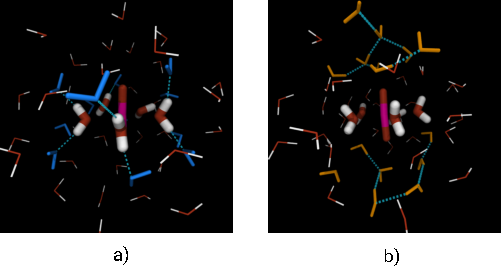
\includegraphics[width=10cm]{./images/An_VI_solvation.pdf}
\caption[Snapshots of \ce{[NpO2*(H2O)5]^{2+}} solvation]{MD snapshots of
\ce{[NpO2*(H2O)5]^{2+}} in water. a) Equatorial water molecules solvating the first-shell 
hydrophilically (blue). a) Axial water molecules hydrophobically solvating the \oyl 
atom (orange). }
\label{ActinylSolvation}
\end{figure}


No hydrogen bonding was found between water molecules and the \oyl atoms. This agrees with 
\textit{ab initio} MD 
simulations\cite{JACS_Buhl_2005,JChemPhys_Nichols_2008,JPhysChemA_Frick_2009} and classical 
simulations using 
\textit{ab initio} force 
fields\cite{JACS_Roos_2005,PhysChemChemPhys_Pomogaev_2013,JPhysChemB_Tiwari_2012}. We 
hypothesize that this apical hydrogen bond could be an artifact 
of empirical force fields\cite{JMolStr_Wipff_1996,JPhysChem_Wipff_1993,JPhysChemA_Kerisit_2013} and 
static QM calculations\cite{ChemPhys_Siboulet_2006}. We describe actinyls as anisotropic 
amphiphillic solutes which have a conventional solvation sphere caped at the poles by hydrophobic 
regions. 


Two clear solvation regions are observed. The equatorial region has the typical first-second 
shell
interactions of cations: the first-shell water mo\-le\-cu\-les form two hydrogen bonds with 
the 
second-shell ones, 
i. e. a 
hydrophilic solvation structure. Axially there is a hydrophobic solvation: the water 
mo\-le\-cu\-les 
form 
water-water structures around the \oyl atoms without interacting directionally with it. The final 
picture is that actinyls are amphiphillic anisotropically solvated solutes that have conventional 
cation solvation caped at the poles by hydrophobic regions (Figure \ref{ActinylSolvation}). This 
solvation is very unusual since a very small and highly charged cation holds two distinct
solvation regions.  

The most important achievement of this part of the thesis is the proposal of a general picture 
of the solvation of actinyls. Our view concurs with other works in the 
literature\cite{JACS_Roos_2005,PhysChemChemPhys_Pomogaev_2013,JPhysChemB_Tiwari_2012,JACS_Buhl_2005,
JChemPhys_Nichols_2008,JPhysChemA_Frick_2009}. Nevertheless, our picture stands on the extension of 
a robust methodology due to:
\begin{enumerate}
 \item The ability of the hydrated ion model 
to capture complicated 
many-body effects. 
 \item Our explicit parametrization of 
the bulk-HI interaction which separates our modeling from the rest of \textit{ab 
initio} force fields. Additionally, this interaction is universal among actinyls. 
\item The use of a classical potential allowed reaching larger 
system sizes and timescales than in \textit{ab initio} MD.
\end{enumerate}
\section[Modelling of actinyl EXAFS spectra]{Modelling of actinyl EXAFS 
spectra}\label{ModelXASSpectra}


The theoretical EXAFS spectra of the actinyls was calculated from the MD trajectories using the 
B3LYP level force fields. Here we shall not refer to americyl since its particular case will be 
explained in the next section. The simulated EXAFS spectrum of uranyl gave a reasonable agreement 
with the 
experimental one. Nevertheless, the rest of actinyls showed a qualitative agreement but far 
from that of 
uranyl or of other cations modeled using the group's methodologies. Since uranyl is the only closed 
shell actinyl of the set, we wondered if the potential energy surface used to build the force field 
was biased by the mean-field treatment done by unrestricted DFT in the open-shell systems. The 
NEVPT2 calculations of the actinyls had the effect of lengthening the An-\oyl distance and as a 
result a shortening of the An-\ofs distance. Although the changes are in the order of hundredths of 
an angstrom, these may cause a certain impact on the EXAFS spectra which are quite sensitive to 
structure. 

We calculated the theoretical EXAFS of \ce{[NpO2]^{+}} using the NEVPT2-level \textit{ab initio} 
force field. There was a significant improvement in the correspondence of the spectra with 
experiment with respect to the correspondence obtained using the DFT-level force field. The 
increase of the level of theory produced overall an improvement in the correspondence with 
experiment of the spectra. Nevertheless, the shoulder at low $k$ appears to be the most 
complex to predict since in this region of the spectrum both An-\oyl and An-\ofs have 
significant weight.

\section[Modelling of americyl XAS spectra]{Modelling of americyl XAS spectra}
Our modeling of americyl XAS spectra was an example of how theory and 
experiment can breed deep insights when combined. This part of the project started when trying 
to compare our theoretical americyl spectrum to experiment. We found that the only available 
experimental EXAFS spectrum were of a mixture of Am(VI)/Am(III), 
published in 2016.\cite{JRadioanNucChem_Riddle_2016} The experimentalists 
were unable to disentangle 
the mixture spectrum into the spectra of the two species. In addition, their modeling of the 
EXAFS equation gave some unusual structural parameters. They obtained a Debye-Waller factor for the 
Am-\oyl distance which was higher than for Am-\ofs. This is unusual since covalent bonds as the 
oxo-bond (\ce{Am=O}) 
are generally stiffer than coordinative bonds (Am-\ofs) and thus have lower thermal dispersion. 
With this information in mind we decided to tackle the problem with some of our newly developed 
actinyl force fields.

\begin{figure}
\centering 
\includegraphics[width=0.7\columnwidth]{./images/Exafs.png}
\caption[EXAFS spectra of Am]{L$_\text{3}$-edge $k^2$-weighted EXAFS spectrum of Am 
experimental (dashed) and simulated 
(solid). Top: $Am^{3+}$ aqueous solution experimental\cite{EnvSciTech_Stumpf_2006} and simulated 
spectra. Middle: pure \ce{[AmO2]^{2+}} simulated spectrum (red) and of the ionic 
mixture\cite{JRadioanNucChem_Riddle_2016}. Bottom: Experimental spectrum of the ionic 
mixture\cite{JRadioanNucChem_Riddle_2016} and simulated spectrum of \ce{[AmO2]^{2+}} and 
\ce{Am^{3+}} weighted with  70/30 (pink) and 55/45 (blue) ratios.}
\label{XAS_Am}
\end{figure}

MD simulations of aqueous \ce{[AmO2*(H2O)5]^{2+}} and 
\ce{[Am*(H2O)8]^{3+}} were run  using the newly developed force fields; \textit{ab initio} for 
Am(VI) and empirical for Am(III). The theoretical EXAFS and XANES spectra for both compounds were 
calculated. The Am(III) spectra matched the experiment as expected since the potential was built 
\textit{ad hoc} to do so. We 
generated the weighted sum of the XAS spectra of both pure 
theoretical spectra to produce the theoretical spectrum of the mixture. The weights were given 
according to the relative abundance of the species reported by the experimentalists. The agreement 
of the theoretical spectrum of the mixture and experiment was really good. The 
experimentalists determined that the initial Am(VI)/Am(III) ratio of the species, 70/30, was 
likely 
to have changed 
due to radiation damage or the redox instability Am(VI). Varying the weights of the simulated 
spectra of Am(VI)/Am(III) we found a 55/45 ratio to give the best match between the experimental 
and theoretical spectra (Figure \ref{XAS_Am}). 

In this work we simulated XAS spectra (EXAFS and XANES) of a 
mixture of species which is consistent with the experiment. This is a very stimulating 
result given the complexity of EXAFS modeling in general, specially on actinyls (see 
Chapter \ref{art3.5}) and in a mixture of species. The results provide confidence in the 
developed methodology.

This synergic theoretical-experimental findings gave strong evidence that our simulation of 
\ce{[AmO2*(H2O)5]^{2+}} was fairly accurate. This allowed us to predict the distances,
Debye-Waller factors and XAS spectra of pure americyl aqueous solution, which has never been 
obtained experimentally. In addition, our parameters recover the usual trend that the stronger 
bond 
should 
have the 
lowest Debye-Waller factor.

\section[Diffusion of uranyl in montmorillonite clay]{Diffusion of uranyl in montmorillonite 
clay}

MD simulations were run on hydrated montmorillonite clay introducing uranyl cations 
in the interlayer in exchange for the \ce{Na+} cations. We studied the diffusion and dynamics of 
the uranyl cations inside the interlayers. Two simulations were run. One contained a single 
uranyl cation 
per interlayer and the other one four ions per interlayer. 
We have studied only uranyl 
but given the similarities between the actinyls, the information is likely to be extended to 
the rest of them. This is particularly important since the most hazardous actinoids of spent 
nuclear 
fuel are neptunium,plutonium and americium.

\begin{figure}
\centering 
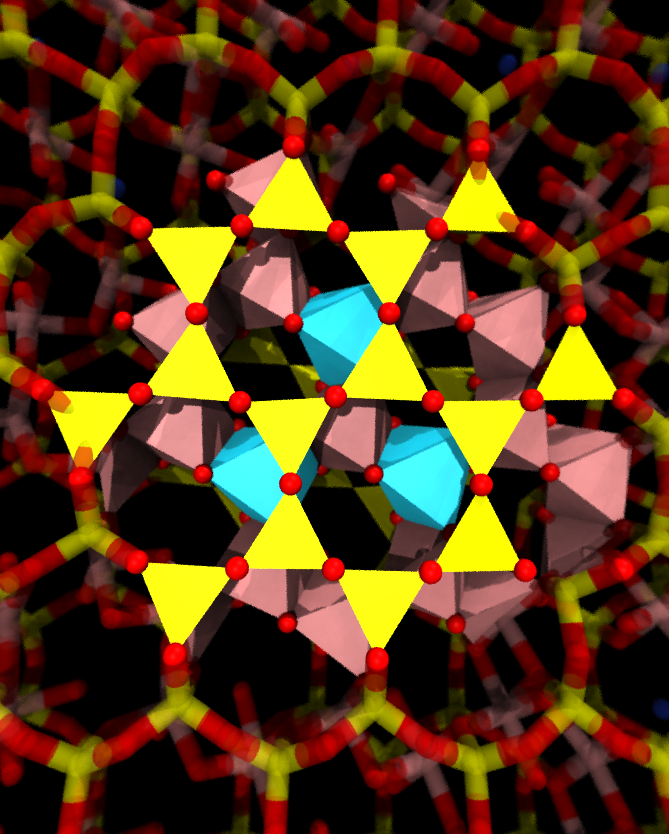
\includegraphics[width=5cm]{./images/site.png}
\caption[Strong interaction site for uranyl]{Interaction site for uranyl at the 
montmorillonite clay surface: three Mg octahedra 
separated from each other by a single central Al octahedron. Al 
octahedra (pink), Mg octahedra (blue), Si tetrahedra (yellow), O atoms (red), uranium atoms 
(green), and H atoms (white) 
}
\label{site}
\end{figure}

The diffusion of the uranyl cations within the clays was greatly hindered with respect to solution. 
The diffusion occurs 
on the clay surface with very few transitions of the cations from one surface to the middle of the 
interlayer or the other surface. This work is the first to calculate from MD the 
constrictivity factor,
$\delta_{int}$, which measures the uranyl diffusivity in the interlayer with respect to 
solution. Our estimation of $\delta_{int}$ was close to one order of magnitude higher than 
experiment\cite{TaiMine_Moore_2011} encouraging the idea that on broad strokes 
we capture the physics of the system. The disagreement between theory and experiment should be put 
in context with the difficulties of modeling a very homogeneous system like real clays in 
complex electrolytes. The main causes of  discrepancy could be the 
relatively short-time of the simulation, the inaccuracies in force field development, the 
differences between our idealized system and the real clays, and the fact that the $\delta_{int}$ 
is a fitted parameter in Fick-equation modeling and other effects could contribute. 

The key finding of the work was the identification of strong interaction sites for uranyl. We 
observed that 
uranyls tightly bound to the surface in regions were three 
substitutions occurred forming a triangle of Mg-octahedra around an Al-octahedron (See 
Figure \ref{site}). The electrostatic potential maps of 
the surface showed that the strong interaction is driven by electrostatics. The identification 
of the sites allowed us to propose a hopping diffusion me\-cha\-nism. In this mechanism the 
uranyl 
cations oscillate around the interaction sites until they are able to escape and diffuse away 
until reaching another site, then the motion becomes oscillatory again. 

The other interesting result of the simulations was that increasing the concentration of 
uranyl cations in the clay increased their diffusion. We found the explanation for this 
phenomenon in the strong interaction sites. If there are more uranyl cations in the interlayer 
there will be more occupied sites on average and thus a diffusing cation will have larger 
displacements before falling into a site. In addition, the repulsion between cations can promote 
one cation ``pushing'' others out of their sites also increasing diffusion. 

The microscopical information obtained from our studies 
gives a complementary view to uranyl diffusion in clays to what is typically studied with 
macroscopic Fick-equation modeling.

\section[Development of a local hydrophobicity/hydrophilicity fingerprint]{Development of a 
local hydrophobicity/hydrophilicity fingerprint for enhanced 
sampling 
simulation}

A local fingerprint for hydrophobicity and hydrophilicity was developed inspired by the 
expansion 
of entropy in terms of increasing correlation terms (Equation \ref{expansion}). The fingerprint 
for solute heavy atom, $i$, in aqueous solution is:
\begin{equation}
S_{\text{s}}^{i}=-2\pi \rho_{\text{w,loc}} \int_{0}^{\infty}\left\{\right. g_{i\text{w}
}(r)\ln\left[g_{i\text{w}}(r)\right] 
-g_{i\text{w}} (r)+1\left.\right\}r^2dr
\label{sij}
\end{equation}
Where $\rho_{\text{w,loc}}$ is the local water density around the solute atom and $g_{i\text{w}
}(r)$ is the radial distribution function (\gls{rdf}) of atom $i$ with water molecules, w. 
$S_{\text{s}}^{i}$ is 
then rescaled into  $h_i$, which is defined to be 1 for water and -1 for 
methane to give perspective to the fingerprint numerical values. The reader must be cautioned that 
the fingerprint is not a measurement of hydration entropy, since it is only one term of the 
expansion of the translational entropy of the system. Our goal is to find a fingerprint that 
measures in simple fashion hydrophobicity or hydrophilicity locally. 



\begin{figure}
\centering
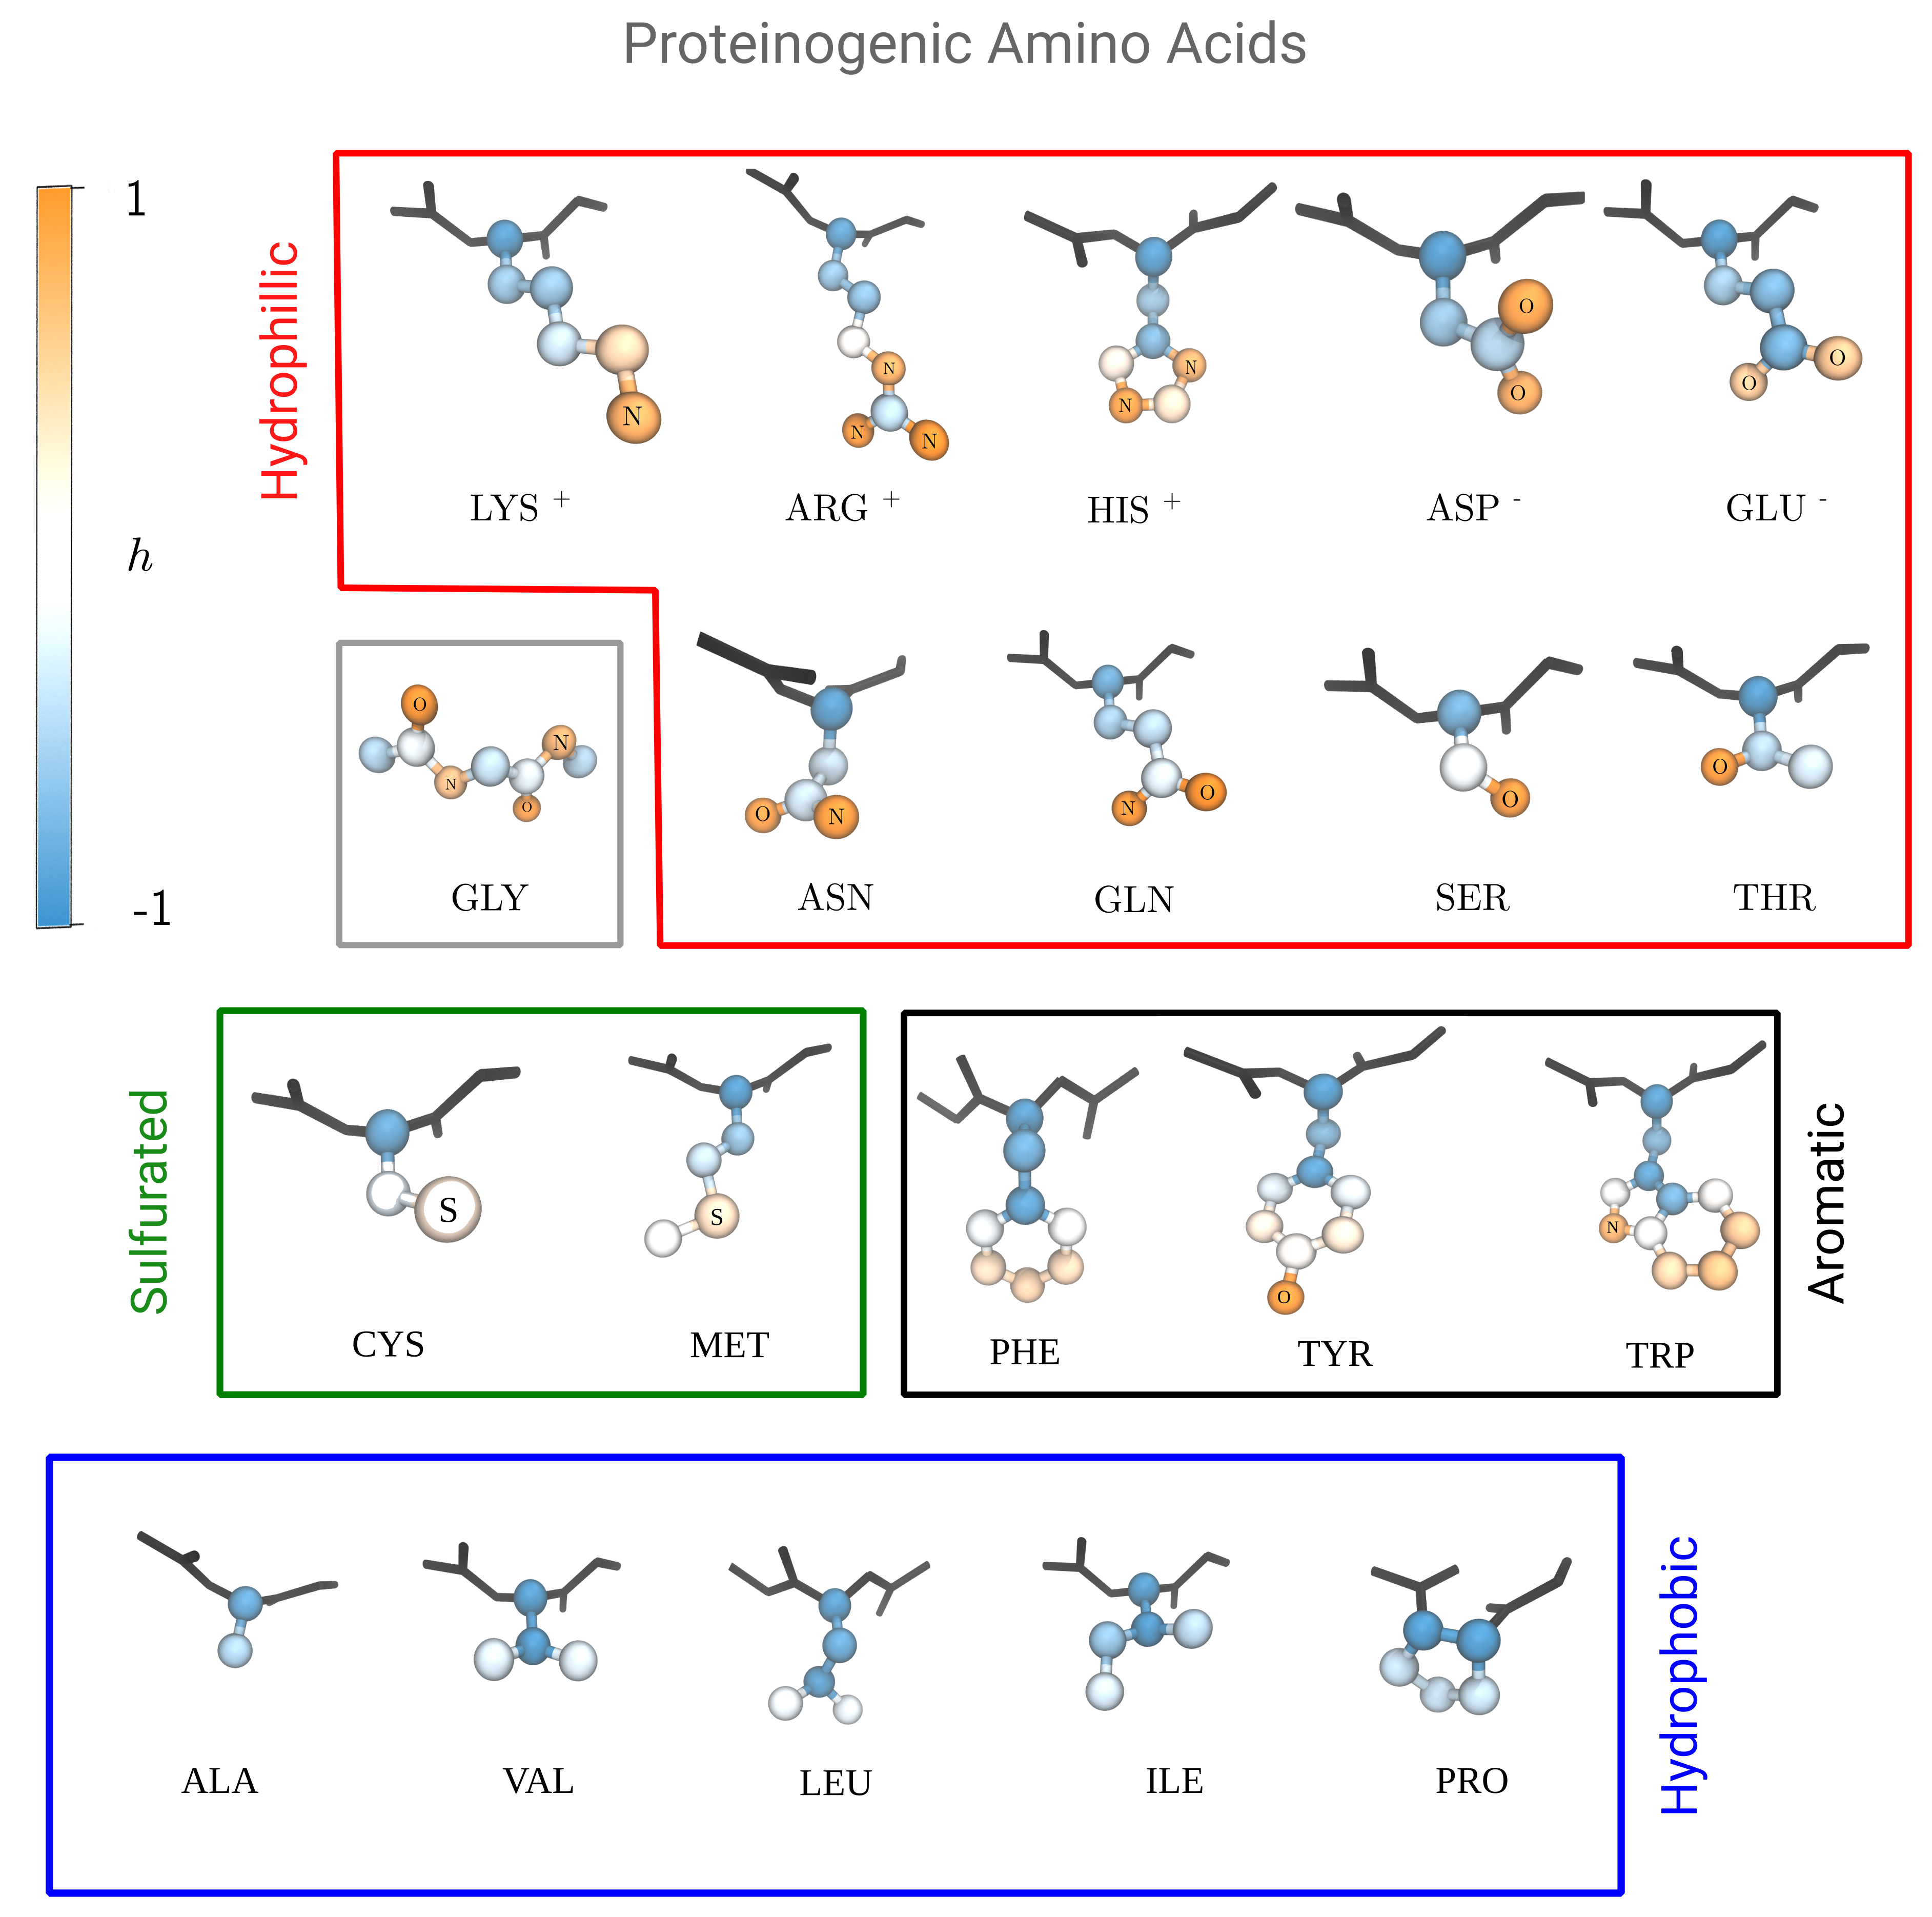
\includegraphics[width=\columnwidth]{./images/aa.png}
\caption[Fingerprint values for the 20 aminoacids]{ Structure of the 20 proteinogenic amino 
acids with their heavy atoms colored by their 
hydrophobicity/hydrophilicity fingerprint values. The color scale varies from hydrophilic 
(orange),
to intermediate (white), to hydrophobic (blue). Hydrogen atoms are omitted. Unlabeled atoms are 
carbon atoms. The backbone is only shown for glycine since its fingerprint value is very similar in 
all cases. }
\label{aa}

\end{figure}
The fingerprint was able to correctly classify as hydrophilic or hydrophobic the atoms of the 
20 
proteinogenic amino acids which have a large variety of chemical groups and  environments. 
Figure \ref{aa} shows the amino acids with their heavy atoms colored 
according to their $h$ values. It is striking that some of 
the aromatic atoms are colored as 
slightly hydrophilic. Interestingly this can be explained because experimentally the 
properties of 
aromatic compounds are not as hydrophobic as aliphatic 
carbons\cite{JPhysChem_McAuliffe_1966,JSolvChem_Cabani_1981,Ben-Amotz2016,Harris2016}. 

The fingerprint is very 
simple in formulation and calculation. It just takes as input the RDF which is routinely 
obtained in simulation. It is a local fingerprint 
that measures atomic hydrophobicity/hydrophilicity in contrast with most scales in the 
literature which focus on the whole residue\cite{Simm2016}. The maximum fingerprint value of 
the amino acid was found to correlate with its hydration free energy. The correlation is not 
very strong but is very similar to the one obtained by Schauperl et al\cite{Schauperl2016}. In 
their 
work they used a much more complex and computationally demanding technique that unlike our 
fingerprint is dedicated fully to thermodynamical property calculation. Therefore, our 
fingerprint gives a measurement of the hydrophobicity or hydrophilicity which is simple, 
local, inexpensive and useful to classify the atoms of molecular solutes. 

The instantaneous value of the fingerprint can be calculated on-the-fly in MD
simulation. The fingerprint can become a CV in enhanced sampling simulations using a 
differentiable continuous version of the RDF. The fingerprint serves as a 
desolvation CV. In order to prove the usefulness of the fingerprint as a 
CV, we ran WTMetaD simulations. The model system chosen was a host-guest system in 
aqueous solution. Host-guest systems are model systems for protein-ligand complexes. The 
host is a barrel-shaped molecule that can host a smaller molecule, the guest. In this system 
in 
particular the literature showed that desolvation of the host was a crucial slow mode of 
the binding\cite{Bhakat2017a}. Therefore, in addition to a binding CV (a contact map) a 
desolvation CV (the fingerprint CV) had to be used in order to converge the simulations.

Using the 
fingerprint as a desolvation CV allowed the convergence of the WTMetaD simulations. 
This was done in a single simulation whereas in the literature it required an 
additional free energy perturbation calculation\cite{Bhakat2017a}. The analysis of the free 
energy surface of the host-guest binding showed that the removal of the two last water 
molecules within the barrel is a kinetic barrier in the process. 

The fingerprint serves as 
an alternative to other solvation CVs like the coordination number of water molecules which just 
counts the number of water molecules around a solute atom. Our CV is more detailed since apart from 
measuring the amount of solvation around the molecule it also accounts for the structure 
of this solvation.

\subsection[Application to actinyl hydration]{Application to actinyl hydration}

 The fingerprint of the actinyl pentahydrate atoms was calculated. The fingerprint has mixed 
results in classifying the atoms of the actinyl pentahydrates and appears to be too coarse for 
such systems. The fingerprint mistakenly classifies the actinoid atom as hydrophobic. This had 
also been observed in \ce{Na+}. It also mislabels the \oyl atom as hydrophilic. We attribute 
this fact to the use of the total RDF which captures the water molecules of the 
bridge-solvation region that do not directly solvate the \oyl atom. Using an angle-solved RDF 
in the fingerprint correctly classifies both oxygen atom types but unfortunately considers the 
\ofs atom less 
hydrophilic than bulk water. 

A future improved fingerprint should probably make use of orientational pair entropy in 
addition to some technique to consider the anisotropicity of the solute in complex 
environments.


\bibliographystyle{achemso}
\bibliography{./library,./extrabib}
     % Capítulo 4
\ChapFrame
\chapter[Conclusions]{Conclusions}\label{c5:conclusion}
In this thesis we have presented a set of \textit{ab initio} HIM force fields for 
\ce{[AnO2*(H2O)5]^{2+}} for An=U, Np, Pu, Am in water as well as an additional one for the 
interaction 
of 
uranyl with montmorillonite clay. These interaction potentials offer an alternative to current 
ones in particular since they pa\-ra\-me\-tri\-ze the HI-bulk water interactions. They have 
proven to reproduce satisfactorily many experimental properties of the systems: XAS spectra, 
hydration enthalpies, diffusion coefficients...

The developed potentials allowed the detailed study of the solvation of the actinyls. Their 
solvation 
was found to be amphiphillic and anisotropic which is remarkable considering the small size of the 
ion 
and its charge. From the MD simulations we calculated the XAS spectra of the 
actinyls and compared then to experiment. This allowed us to assess the quality of their structural 
model and to interpret the keys of their complex spectra. In particular, we 
interpreted the experimental XAS spectra of an \ce{Am^{3+}}/\ce{[AmO2]^{2+}} mixture 
reproducing the 
theoretical EXAFS spectrum of a mixture. With the experimental validation of our 
simulation we were able to predict the structural parameters and the EXAFS and XANES spectra of a 
pure 
\ce{[AmO2*(H2O)5]^{2+}} solution, a solution that has never been obtained. This will be a 
striking experimental challenge for actinoid solution chemistry in the near future.

The uranyl montmorillonite clay simulations allowed us to study the diffusion of the HI in the 
interlayers. We identified the existence of strong interaction sites for uranyl. These sites force 
the uranyl to diffuse following a hopping mechanism. Because of this,
uranyl diffusion increases with uranyl concentration due to cation-cation interactions 
and a larger coverage of 
surface sites.

Another methodological achievement of this thesis has been the development of a simple local 
fingerprint for hydrophobicity and hydrophilicity. The fingerprint was able to classify 
correctly 
the atoms of amino acids in water which have varied functional groups and chemical 
environments. The fingerprint has also been proven to be a useful solvation/desolvation CV in 
enhanced sampling simulations. When applied to characterize the different hydration regions 
around actinyls, fingerprint values do not seem to provide such a clear view as in the amino 
acid case. This opens the door to refinement of the index when dealing with metal cations and 
ions in general.
 

In conclusion, this thesis provides a different perspective to the study of aqueous actinyls and 
actinyls in clay interlayers. This different perspective is based on the usage of newly developed 
methodologies that enable a cost effective and fairly accurate view of these important systems. 
     % Capítulo 5
%%Página EXTRA FINAL
% only if A4
\pagestyle{empty}
\newpage
\pagestyle{empty}
\ 
\newpage
\ 
\newpage
\end{document}   % FIN DE DOCUMENTO

